\documentclass[aspectratio=1610]{beamer}

\usetheme{KTH}

% remove this if using XeLaTeX or LuaLaTeX
\usepackage[utf8]{inputenc}

\usepackage{wrapfig}
\usepackage{subcaption}

\usepackage{tikz}
\usepackage{array}

\usepackage[export]{adjustbox}

\usepackage{keyval}
\usepackage{ifthen}
%====================================
%emphasize vertices --> switch and emph style (e.g. thick,black)
%====================================
\makeatletter
% Standard Values for Parameters
\newcommand{\tikzcuboid@shiftx}{0}
\newcommand{\tikzcuboid@shifty}{0}
\newcommand{\tikzcuboid@dimx}{3}
\newcommand{\tikzcuboid@dimy}{3}
\newcommand{\tikzcuboid@dimz}{3}
\newcommand{\tikzcuboid@scale}{1}
\newcommand{\tikzcuboid@densityx}{1}
\newcommand{\tikzcuboid@densityy}{1}
\newcommand{\tikzcuboid@densityz}{1}
\newcommand{\tikzcuboid@rotation}{0}
\newcommand{\tikzcuboid@anglex}{0}
\newcommand{\tikzcuboid@angley}{90}
\newcommand{\tikzcuboid@anglez}{225}
\newcommand{\tikzcuboid@scalex}{1}
\newcommand{\tikzcuboid@scaley}{1}
\newcommand{\tikzcuboid@scalez}{sqrt(0.5)}
\newcommand{\tikzcuboid@linefront}{black}
\newcommand{\tikzcuboid@linetop}{black}
\newcommand{\tikzcuboid@lineright}{black}
\newcommand{\tikzcuboid@fillfront}{white}
\newcommand{\tikzcuboid@filltop}{white}
\newcommand{\tikzcuboid@fillright}{white}
\newcommand{\tikzcuboid@shaded}{N}
\newcommand{\tikzcuboid@shadecolor}{black}
\newcommand{\tikzcuboid@shadeperc}{25}
\newcommand{\tikzcuboid@emphedge}{N}
\newcommand{\tikzcuboid@emphstyle}{thick}

% Definition of Keys
\define@key{tikzcuboid}{shiftx}[\tikzcuboid@shiftx]{\renewcommand{\tikzcuboid@shiftx}{#1}}
\define@key{tikzcuboid}{shifty}[\tikzcuboid@shifty]{\renewcommand{\tikzcuboid@shifty}{#1}}
\define@key{tikzcuboid}{dimx}[\tikzcuboid@dimx]{\renewcommand{\tikzcuboid@dimx}{#1}}
\define@key{tikzcuboid}{dimy}[\tikzcuboid@dimy]{\renewcommand{\tikzcuboid@dimy}{#1}}
\define@key{tikzcuboid}{dimz}[\tikzcuboid@dimz]{\renewcommand{\tikzcuboid@dimz}{#1}}
\define@key{tikzcuboid}{scale}[\tikzcuboid@scale]{\renewcommand{\tikzcuboid@scale}{#1}}
\define@key{tikzcuboid}{densityx}[\tikzcuboid@densityx]{\renewcommand{\tikzcuboid@densityx}{#1}}
\define@key{tikzcuboid}{densityy}[\tikzcuboid@densityy]{\renewcommand{\tikzcuboid@densityy}{#1}}
\define@key{tikzcuboid}{densityz}[\tikzcuboid@densityz]{\renewcommand{\tikzcuboid@densityz}{#1}}
\define@key{tikzcuboid}{rotation}[\tikzcuboid@rotation]{\renewcommand{\tikzcuboid@rotation}{#1}}
\define@key{tikzcuboid}{anglex}[\tikzcuboid@anglex]{\renewcommand{\tikzcuboid@anglex}{#1}}
\define@key{tikzcuboid}{angley}[\tikzcuboid@angley]{\renewcommand{\tikzcuboid@angley}{#1}}
\define@key{tikzcuboid}{anglez}[\tikzcuboid@anglez]{\renewcommand{\tikzcuboid@anglez}{#1}}
\define@key{tikzcuboid}{scalex}[\tikzcuboid@scalex]{\renewcommand{\tikzcuboid@scalex}{#1}}
\define@key{tikzcuboid}{scaley}[\tikzcuboid@scaley]{\renewcommand{\tikzcuboid@scaley}{#1}}
\define@key{tikzcuboid}{scalez}[\tikzcuboid@scalez]{\renewcommand{\tikzcuboid@scalez}{#1}}
\define@key{tikzcuboid}{linefront}[\tikzcuboid@linefront]{\renewcommand{\tikzcuboid@linefront}{#1}}
\define@key{tikzcuboid}{linetop}[\tikzcuboid@linetop]{\renewcommand{\tikzcuboid@linetop}{#1}}
\define@key{tikzcuboid}{lineright}[\tikzcuboid@lineright]{\renewcommand{\tikzcuboid@lineright}{#1}}
\define@key{tikzcuboid}{fillfront}[\tikzcuboid@fillfront]{\renewcommand{\tikzcuboid@fillfront}{#1}}
\define@key{tikzcuboid}{filltop}[\tikzcuboid@filltop]{\renewcommand{\tikzcuboid@filltop}{#1}}
\define@key{tikzcuboid}{fillright}[\tikzcuboid@fillright]{\renewcommand{\tikzcuboid@fillright}{#1}}
\define@key{tikzcuboid}{shaded}[\tikzcuboid@shaded]{\renewcommand{\tikzcuboid@shaded}{#1}}
\define@key{tikzcuboid}{shadecolor}[\tikzcuboid@shadecolor]{\renewcommand{\tikzcuboid@shadecolor}{#1}}
\define@key{tikzcuboid}{shadeperc}[\tikzcuboid@shadeperc]{\renewcommand{\tikzcuboid@shadeperc}{#1}}
\define@key{tikzcuboid}{emphedge}[\tikzcuboid@emphedge]{\renewcommand{\tikzcuboid@emphedge}{#1}}
\define@key{tikzcuboid}{emphstyle}[\tikzcuboid@emphstyle]{\renewcommand{\tikzcuboid@emphstyle}{#1}}
% Commands
\newcommand{\tikzcuboid}[1]{
    \setkeys{tikzcuboid}{#1} % Process Keys passed to command
    \pgfmathsetmacro{\vectorxx}{\tikzcuboid@scalex*cos(\tikzcuboid@anglex)}
    \pgfmathsetmacro{\vectorxy}{\tikzcuboid@scalex*sin(\tikzcuboid@anglex)}
    \pgfmathsetmacro{\vectoryx}{\tikzcuboid@scaley*cos(\tikzcuboid@angley)}
    \pgfmathsetmacro{\vectoryy}{\tikzcuboid@scaley*sin(\tikzcuboid@angley)}
    \pgfmathsetmacro{\vectorzx}{\tikzcuboid@scalez*cos(\tikzcuboid@anglez)}
    \pgfmathsetmacro{\vectorzy}{\tikzcuboid@scalez*sin(\tikzcuboid@anglez)}
    \begin{scope}[xshift=\tikzcuboid@shiftx, yshift=\tikzcuboid@shifty, scale=\tikzcuboid@scale, rotate=\tikzcuboid@rotation, x={(\vectorxx,\vectorxy)}, y={(\vectoryx,\vectoryy)}, z={(\vectorzx,\vectorzy)}]
    \pgfmathsetmacro{\steppingx}{1/\tikzcuboid@densityx}
    \pgfmathsetmacro{\steppingy}{1/\tikzcuboid@densityy}
    \pgfmathsetmacro{\steppingz}{1/\tikzcuboid@densityz}
    \newcommand{\dimx}{\tikzcuboid@dimx}
    \newcommand{\dimy}{\tikzcuboid@dimy}
    \newcommand{\dimz}{\tikzcuboid@dimz}
    \pgfmathsetmacro{\secondx}{2*\steppingx}
    \pgfmathsetmacro{\secondy}{2*\steppingy}
    \pgfmathsetmacro{\secondz}{2*\steppingz}
    \foreach \x in {\steppingx,\secondx,...,\dimx}
    {   \foreach \y in {\steppingy,\secondy,...,\dimy}
        {   \pgfmathsetmacro{\lowx}{(\x-\steppingx)}
            \pgfmathsetmacro{\lowy}{(\y-\steppingy)}
            \filldraw[fill=\tikzcuboid@fillfront,draw=\tikzcuboid@linefront] (\lowx,\lowy,\dimz) -- (\lowx,\y,\dimz) -- (\x,\y,\dimz) -- (\x,\lowy,\dimz) -- cycle;

        }
    }
    \foreach \x in {\steppingx,\secondx,...,\dimx}
    {   \foreach \z in {\steppingz,\secondz,...,\dimz}
        {   \pgfmathsetmacro{\lowx}{(\x-\steppingx)}
            \pgfmathsetmacro{\lowz}{(\z-\steppingz)}
            \filldraw[fill=\tikzcuboid@filltop,draw=\tikzcuboid@linetop] (\lowx,\dimy,\lowz) -- (\lowx,\dimy,\z) -- (\x,\dimy,\z) -- (\x,\dimy,\lowz) -- cycle;
        }
    }
    \foreach \y in {\steppingy,\secondy,...,\dimy}
    {   \foreach \z in {\steppingz,\secondz,...,\dimz}
        {   \pgfmathsetmacro{\lowy}{(\y-\steppingy)}
            \pgfmathsetmacro{\lowz}{(\z-\steppingz)}
            \filldraw[fill=\tikzcuboid@fillright,draw=\tikzcuboid@lineright] (\dimx,\lowy,\lowz) -- (\dimx,\lowy,\z) -- (\dimx,\y,\z) -- (\dimx,\y,\lowz) -- cycle;
        }
    }
    \ifthenelse{\equal{\tikzcuboid@emphedge}{Y}}%
        {\draw[\tikzcuboid@emphstyle](0,\dimy,0) -- (\dimx,\dimy,0) -- (\dimx,\dimy,\dimz) -- (0,\dimy,\dimz) -- cycle;%
        \draw[\tikzcuboid@emphstyle] (0,0,\dimz) -- (0,\dimy,\dimz) -- (\dimx,\dimy,\dimz) -- (\dimx,0,\dimz) -- cycle;%
        \draw[\tikzcuboid@emphstyle](\dimx,0,0) -- (\dimx,\dimy,0) -- (\dimx,\dimy,\dimz) -- (\dimx,0,\dimz) -- cycle;%
        }%
        {}
    \end{scope}
}

\makeatother



\begin{document}

\startpage
%%%%%%%%%%%%%%%%%%%%%%%%%%%%%%%%%%%%%%%%%%%%%%%%%%%%%%%%%%%%
\begin{frame}

  \vspace{0.02\textheight}
  
  \begin{Large}
    Newspaper article segmentation \\
    using Mask R-CNN and Sentence-BERT
  \end{Large}



  \vspace{0.1\textheight}

  \begin{small}
    \textit{Gustav Henning}
  \end{small}
\end{frame}

\normalpage
%%%%%%%%%%%%%%%%%%%%%%%%%%%%%%%%%%%%%%%%%%%%%%%%%%%%%%%%%%%%
\begin{frame}
\begin{figure}
\centering
\begin{subfigure}{0.9\textwidth}
  \centering
  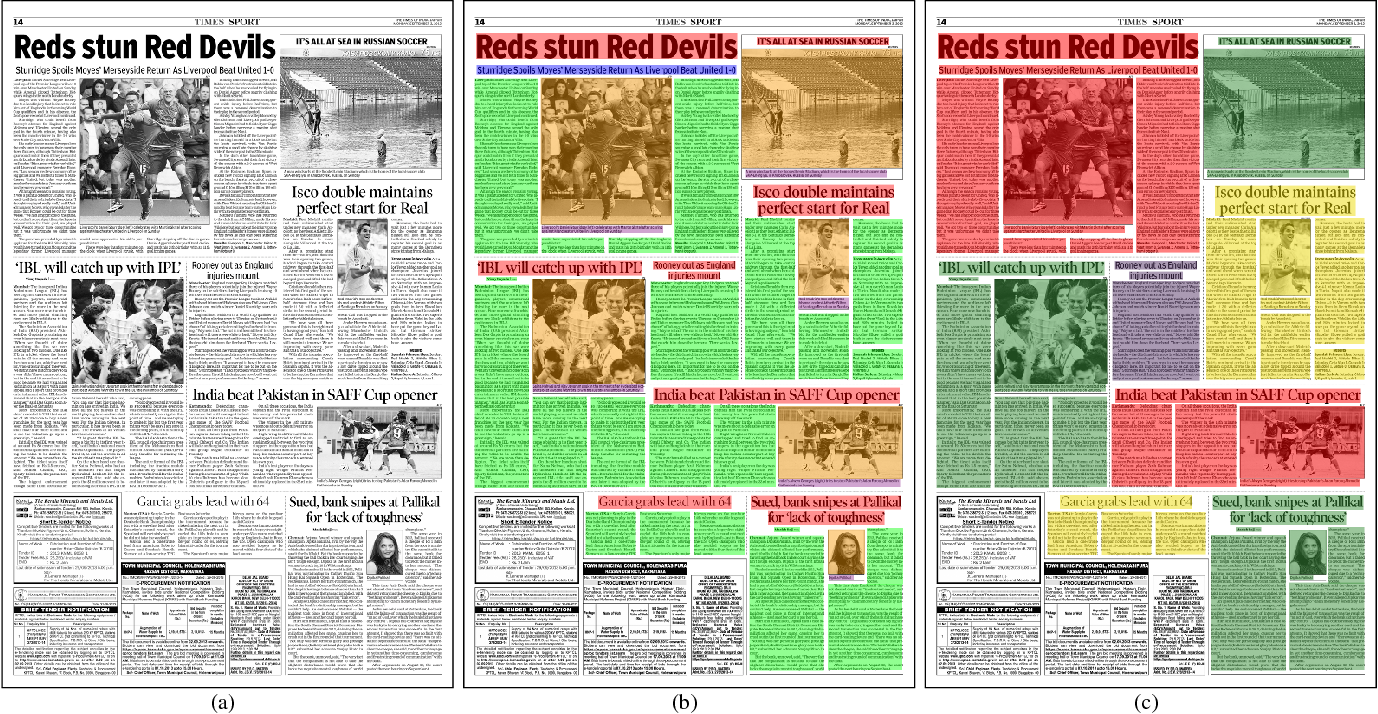
\includegraphics[max size={1.0\textwidth}{1.0\textheight}]{figures/articlesegm.png}
  \label{fig:submscoco}
\end{subfigure}%
  \caption{Example of newspaper article segmentation. [Bansal et al 2014]}
\label{fig:articlesegm}
\end{figure}
\end{frame}
\normalpage


%%%%%%%%%%%%%%%%%%%%%%%%%%%%%%%%%%%%%%%%%%%%%%%%%%%%%%%%%%%%
\begin{frame}
\begin{figure}
\centering
\begin{subfigure}{0.9\textwidth}
  \centering
  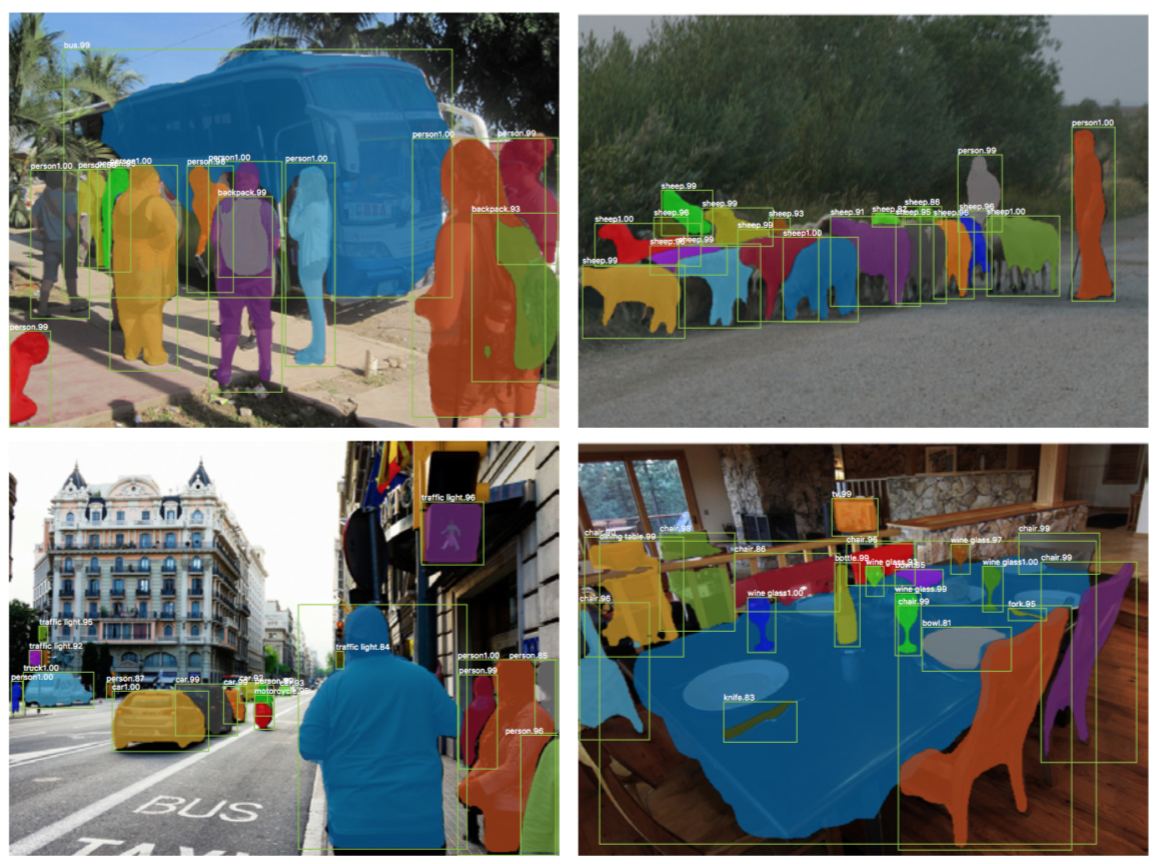
\includegraphics[max size={0.9\textwidth}{0.9\textheight}]{figures/mask-rcnn-examples.png}
  \label{fig:submscoco}
\end{subfigure}%
  \caption{Mask R-CNN output for MS COCO (Common objects in Context). [He et al 2017]}
\label{fig:mscoco}
\end{figure}
\end{frame}
\normalpage

\begin{frame}
  \frametitle{Is this feasible?}


\begin{center}
\begin{tabular}{ |m{15em}|m{5em}|m{15em}| } 
 \hline
 What we require in newspaper article segmentation & Can Mask R-CNN do this? & How? \\ 
 \hline
 Detecting multiple instances of the same class & Yes & Region Proposal Network \\ 
 Detecting objects at different scales & Yes & Feature Pyramid Network \\ 
 Representing several elements as one instance & ? (Yes) & Convolutional Neural Network \\ 
 Comparing texts based on semantics & No & - \\ 
 \hline
\end{tabular}
\end{center}

\end{frame}


%%%%%%%%%%%%%%%%%%%%%%%%%%%%%%%%%%%%%%%%%%%%%%%%%%%%%%%%%%%%
\begin{frame}
\begin{figure}
\centering
\begin{subfigure}{.5\textwidth}
  \centering
  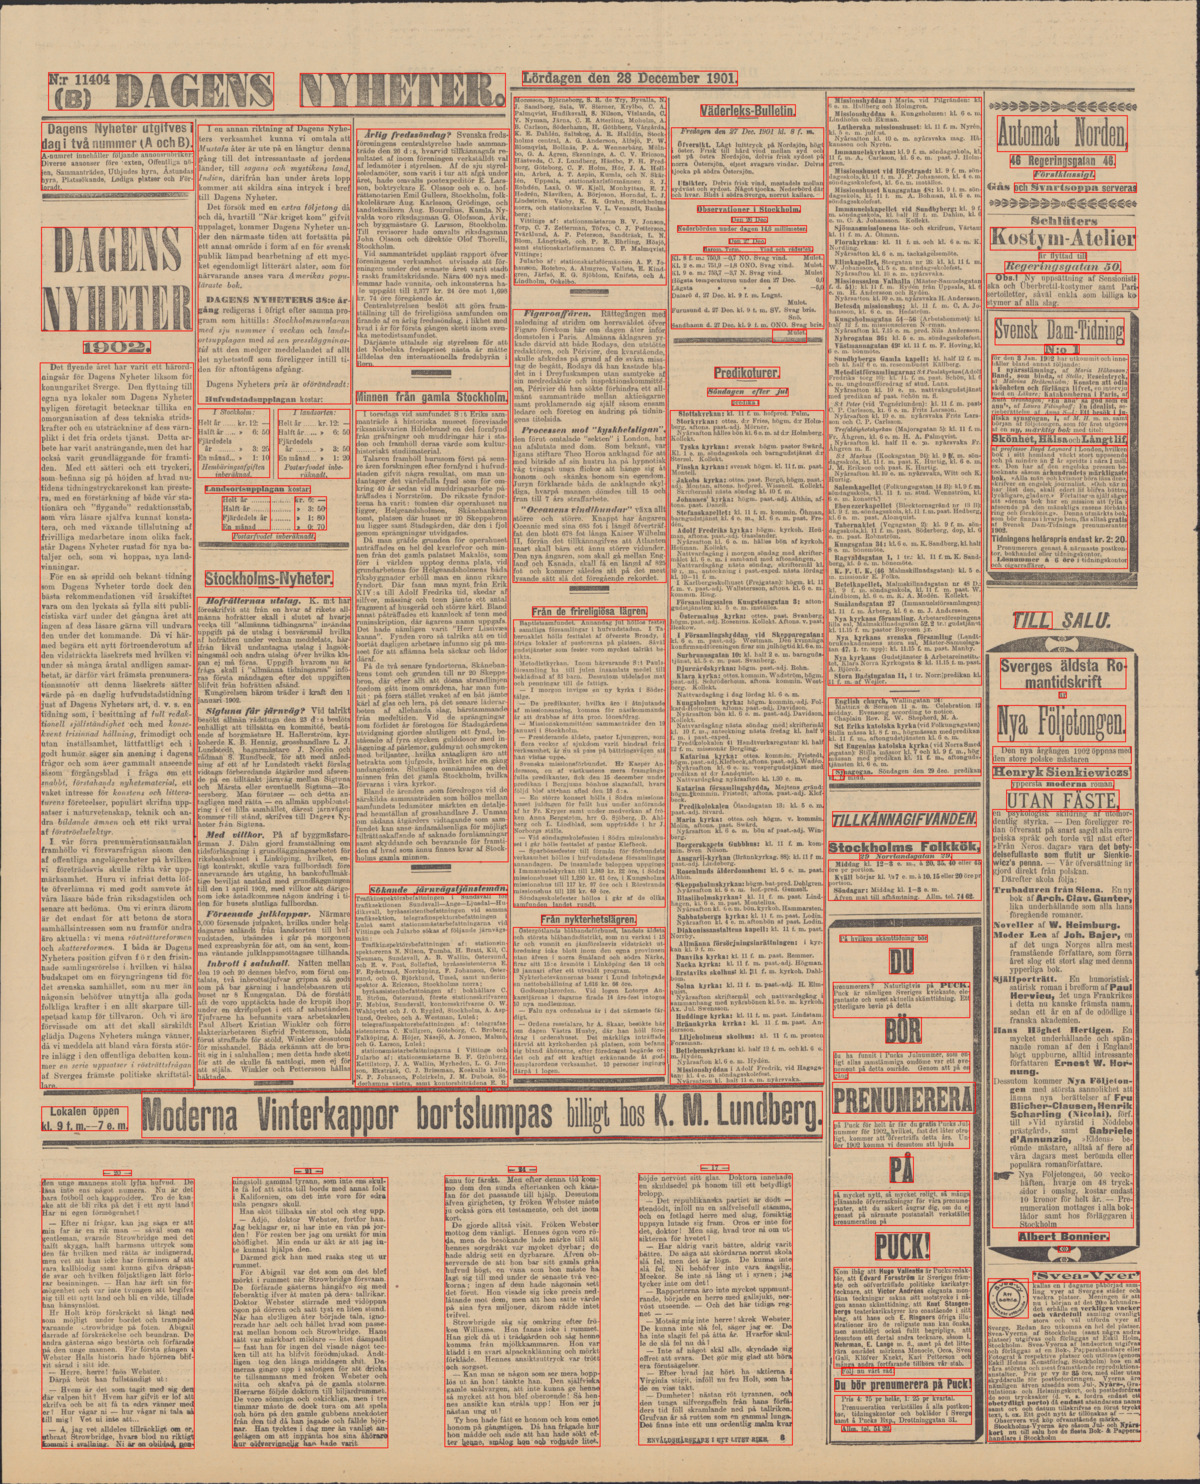
\includegraphics[max size={0.95\textwidth}{0.95\textheight}]{figures/1901-ocr.jpg}
  \caption{OCR bounding boxes visualized in red.}
  \label{fig:raw1901}
\end{subfigure}%
\begin{subfigure}{.5\textwidth}
  \centering
  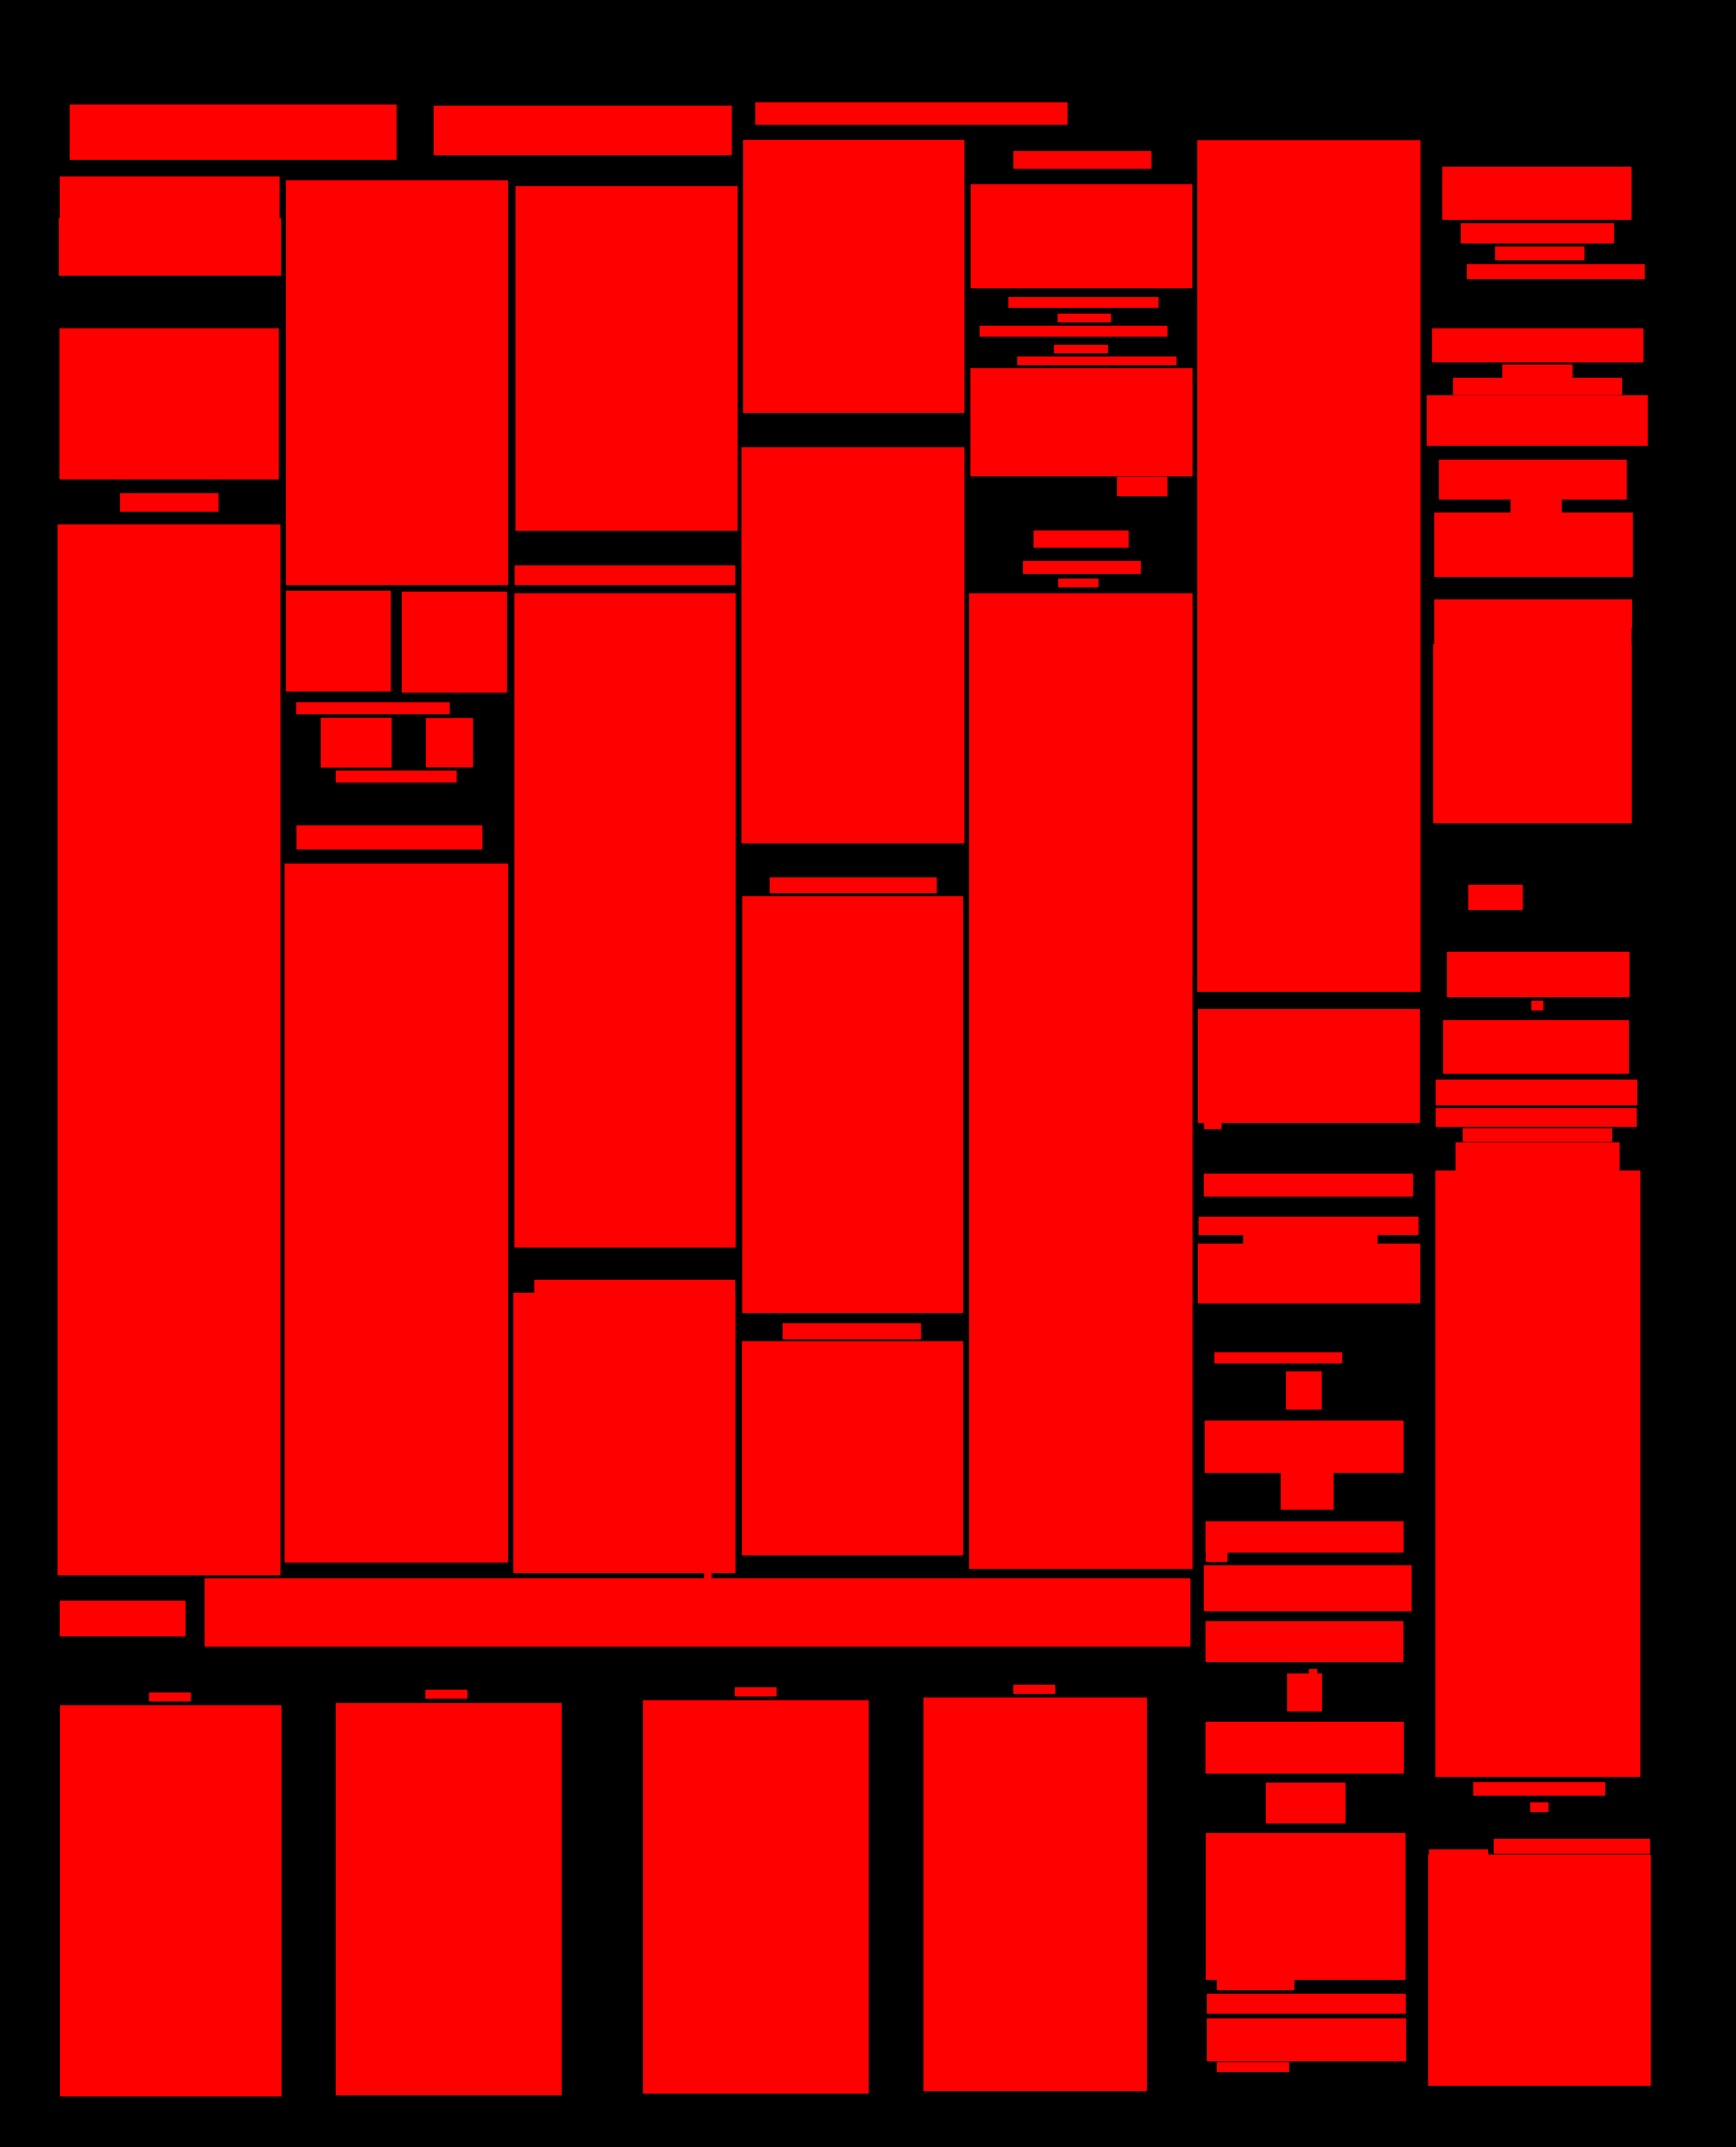
\includegraphics[max size={0.95\textwidth}{0.95\textheight}]{figures/output-black-True.png}
  \caption{OCR visualized in red without raw data.}
  \label{fig:ocr1901}
\end{subfigure}
\label{fig:1901}
\end{figure}

\end{frame}
\normalpage

%%%%%%%%%%%%%%%%%%%%%%%%%%%%%%%%%%%%%%%%%%%%%%%%%%%%%%%%%%%%
\begin{frame}
  \begin{figure}
\centering
\begin{subfigure}{.25\textwidth}
  \centering
  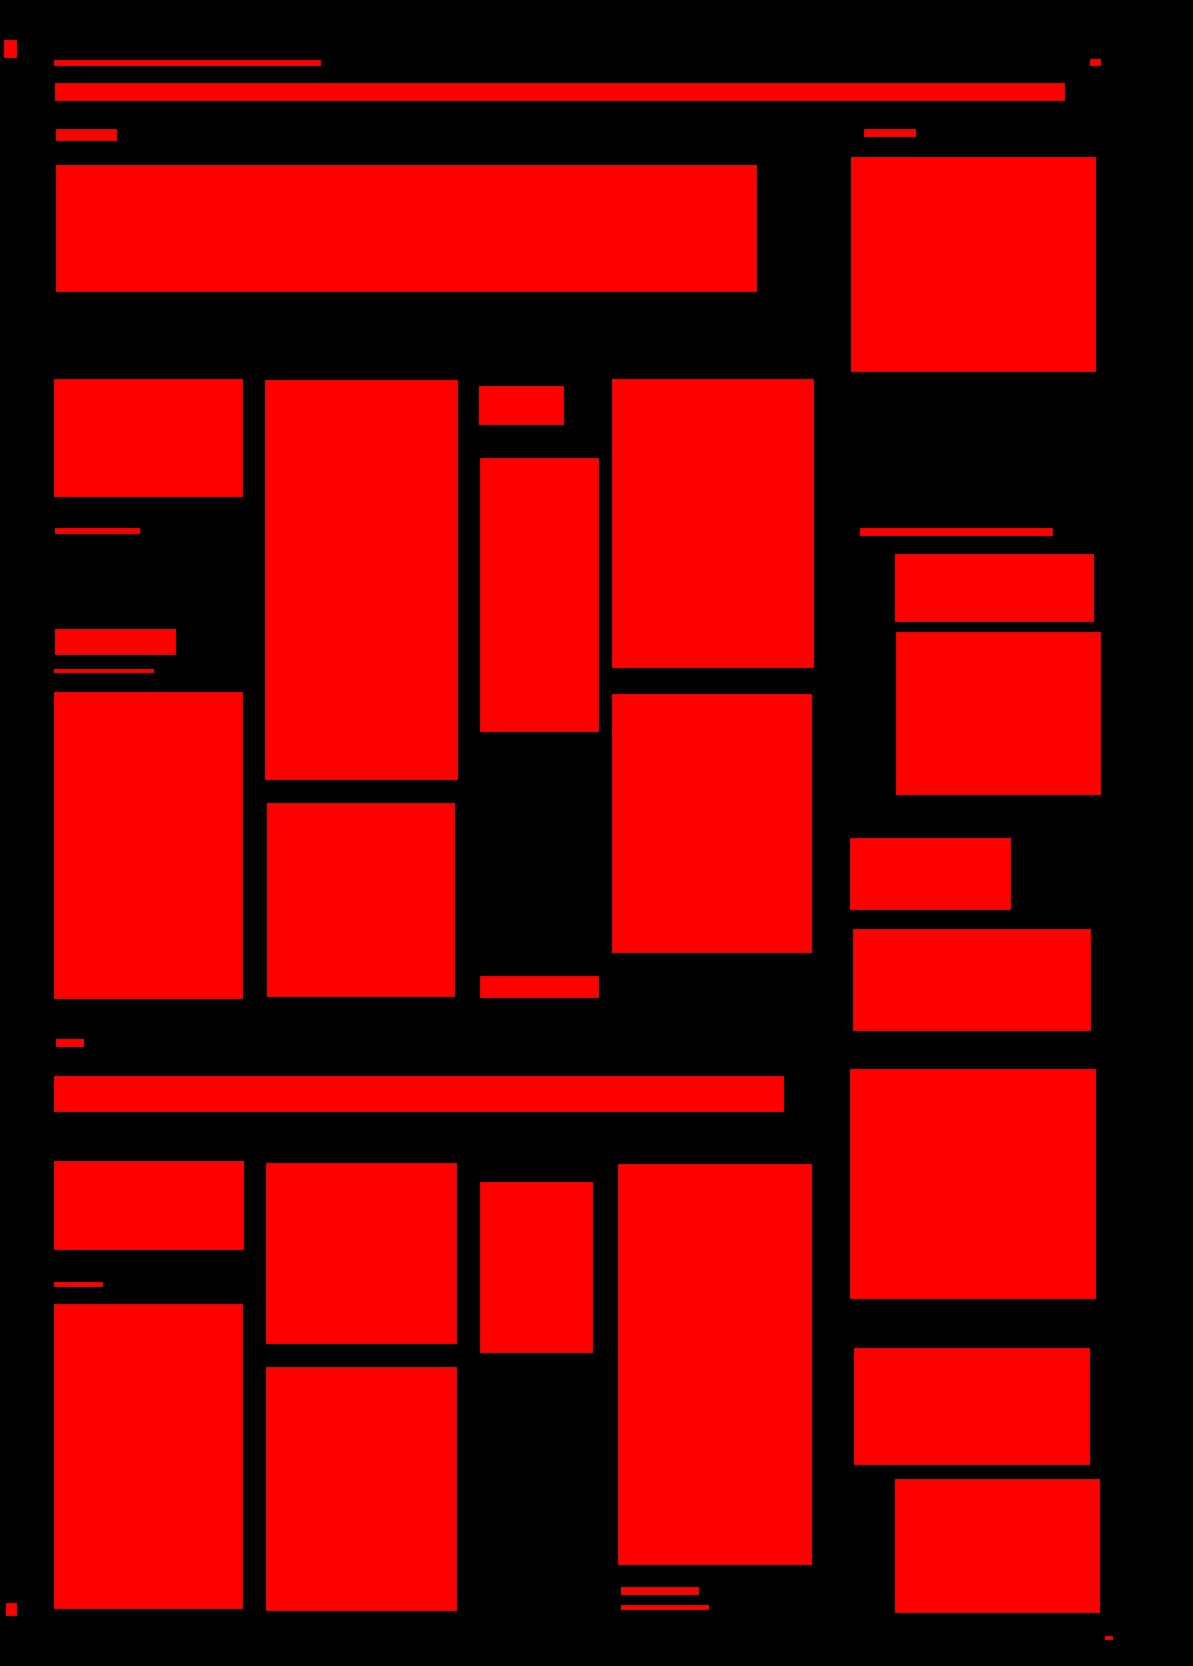
\includegraphics[width=0.99\linewidth, clip=true, trim = 0mm 0mm 0mm 0mm]{figures/ocr/AVThDFz.jpg}
  \caption{OCR}
\end{subfigure}%
\begin{subfigure}{.25\textwidth}
  \centering
  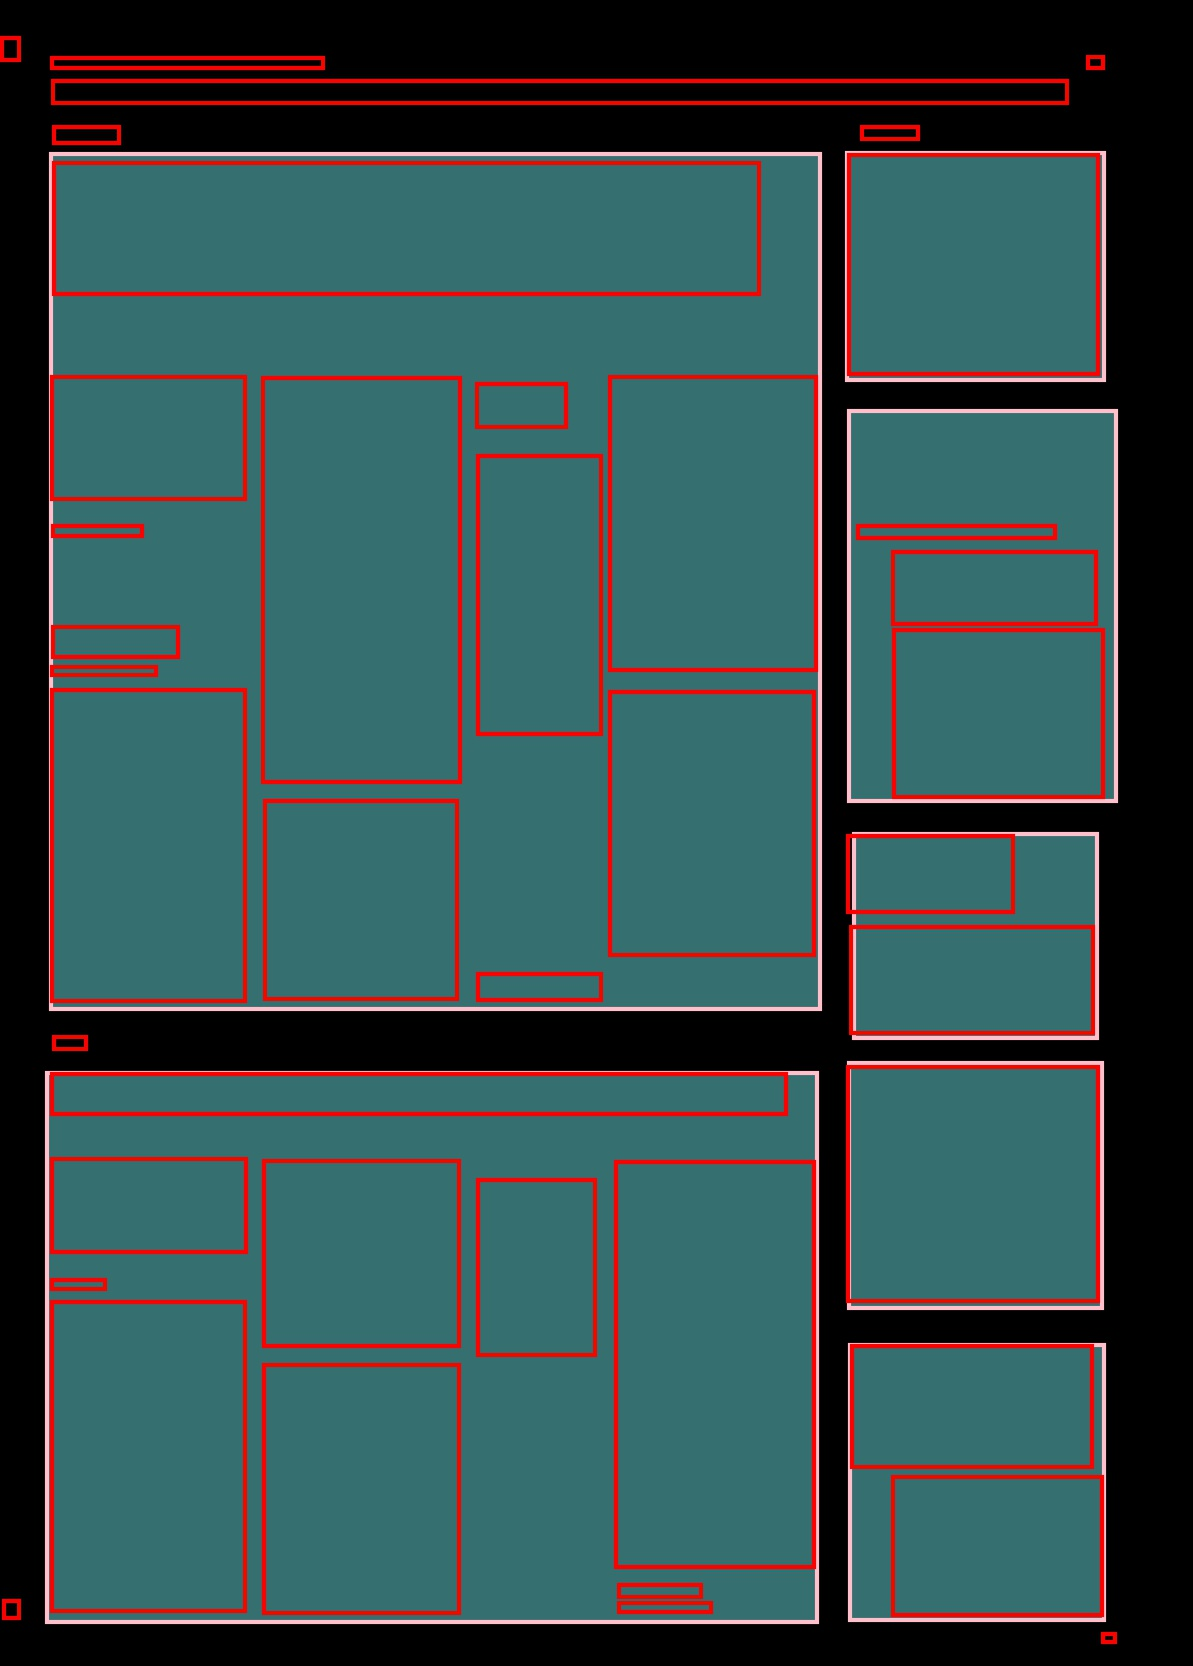
\includegraphics[width=0.99\linewidth, clip=true, trim = 0mm 0mm 0mm 0mm]{figures/ocr_bbox/AVThDFz.jpg}
  \caption{GT Label + OCR}
\end{subfigure}%
\begin{subfigure}{.25\textwidth}
  \centering
  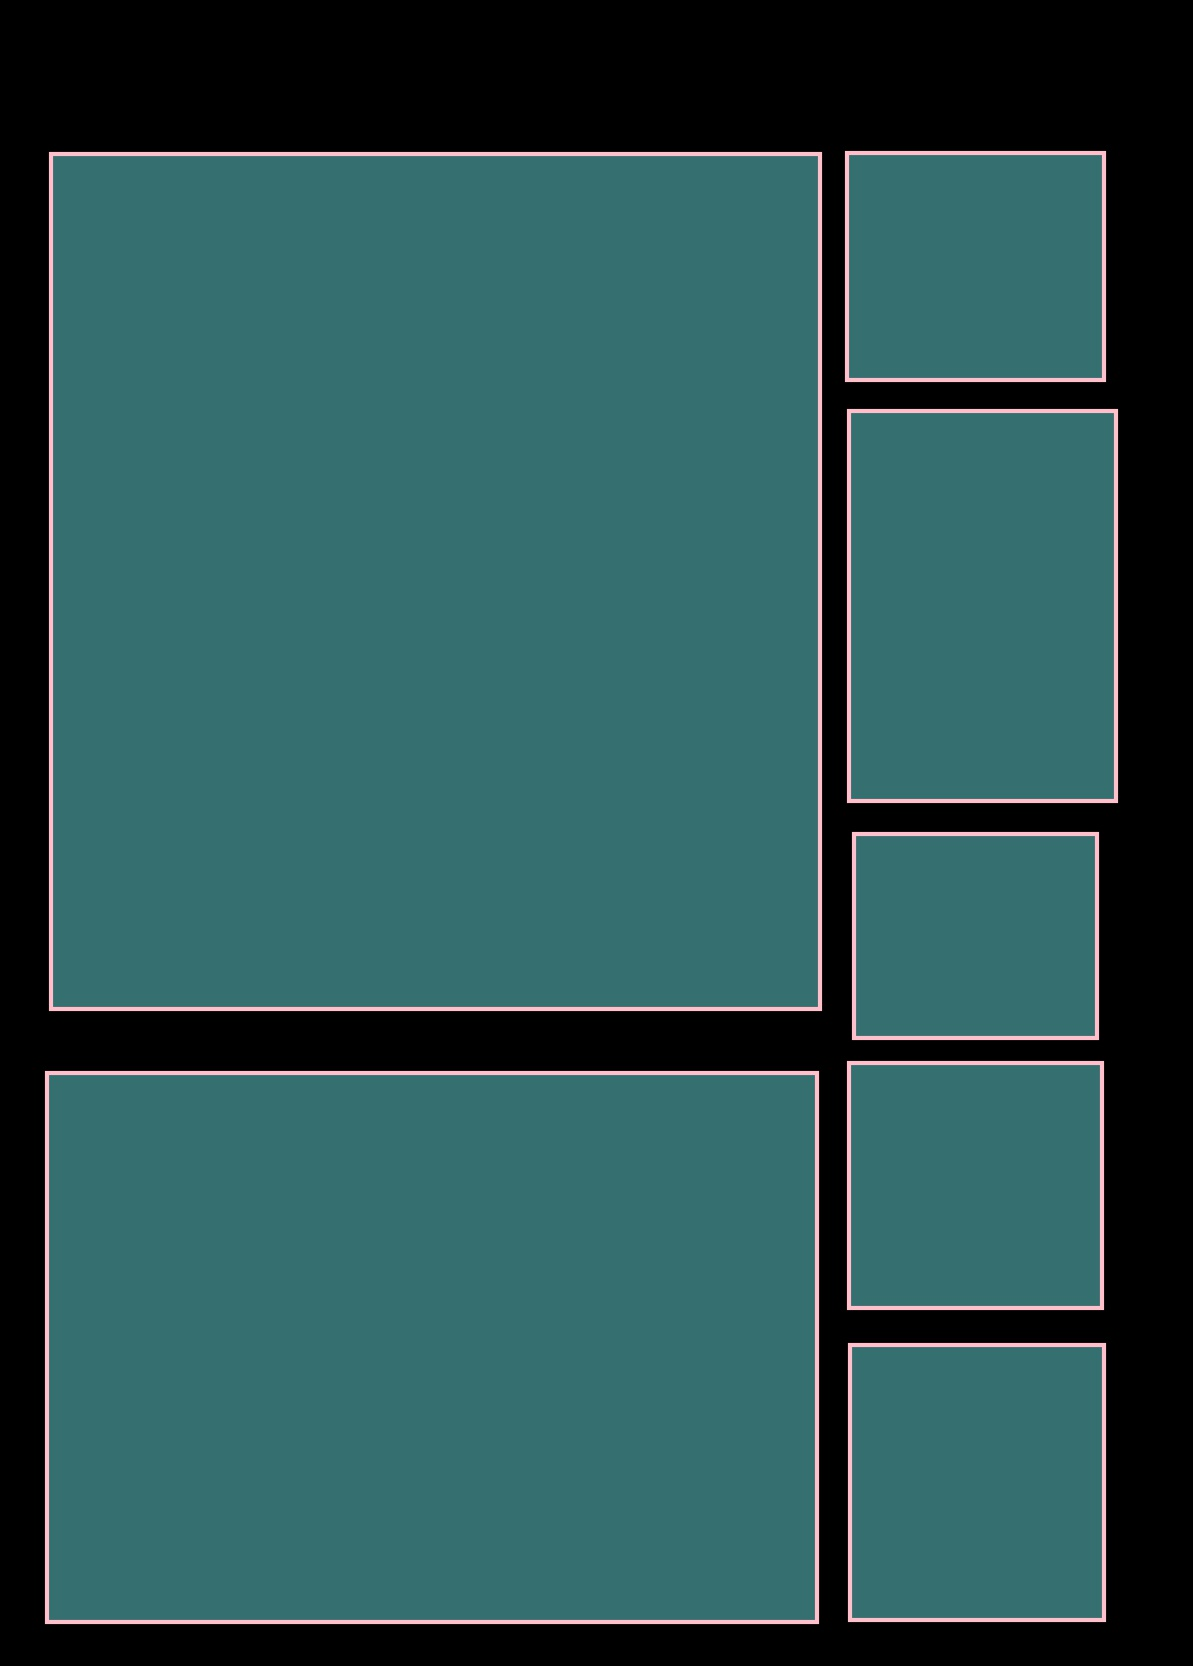
\includegraphics[width=0.99\linewidth, clip=true, trim = 0mm 0mm 0mm 0mm]{figures/bbox/AVThDFz.jpg}
  \caption{GT Label}
\end{subfigure}%
\begin{subfigure}{.25\textwidth}
  \centering
  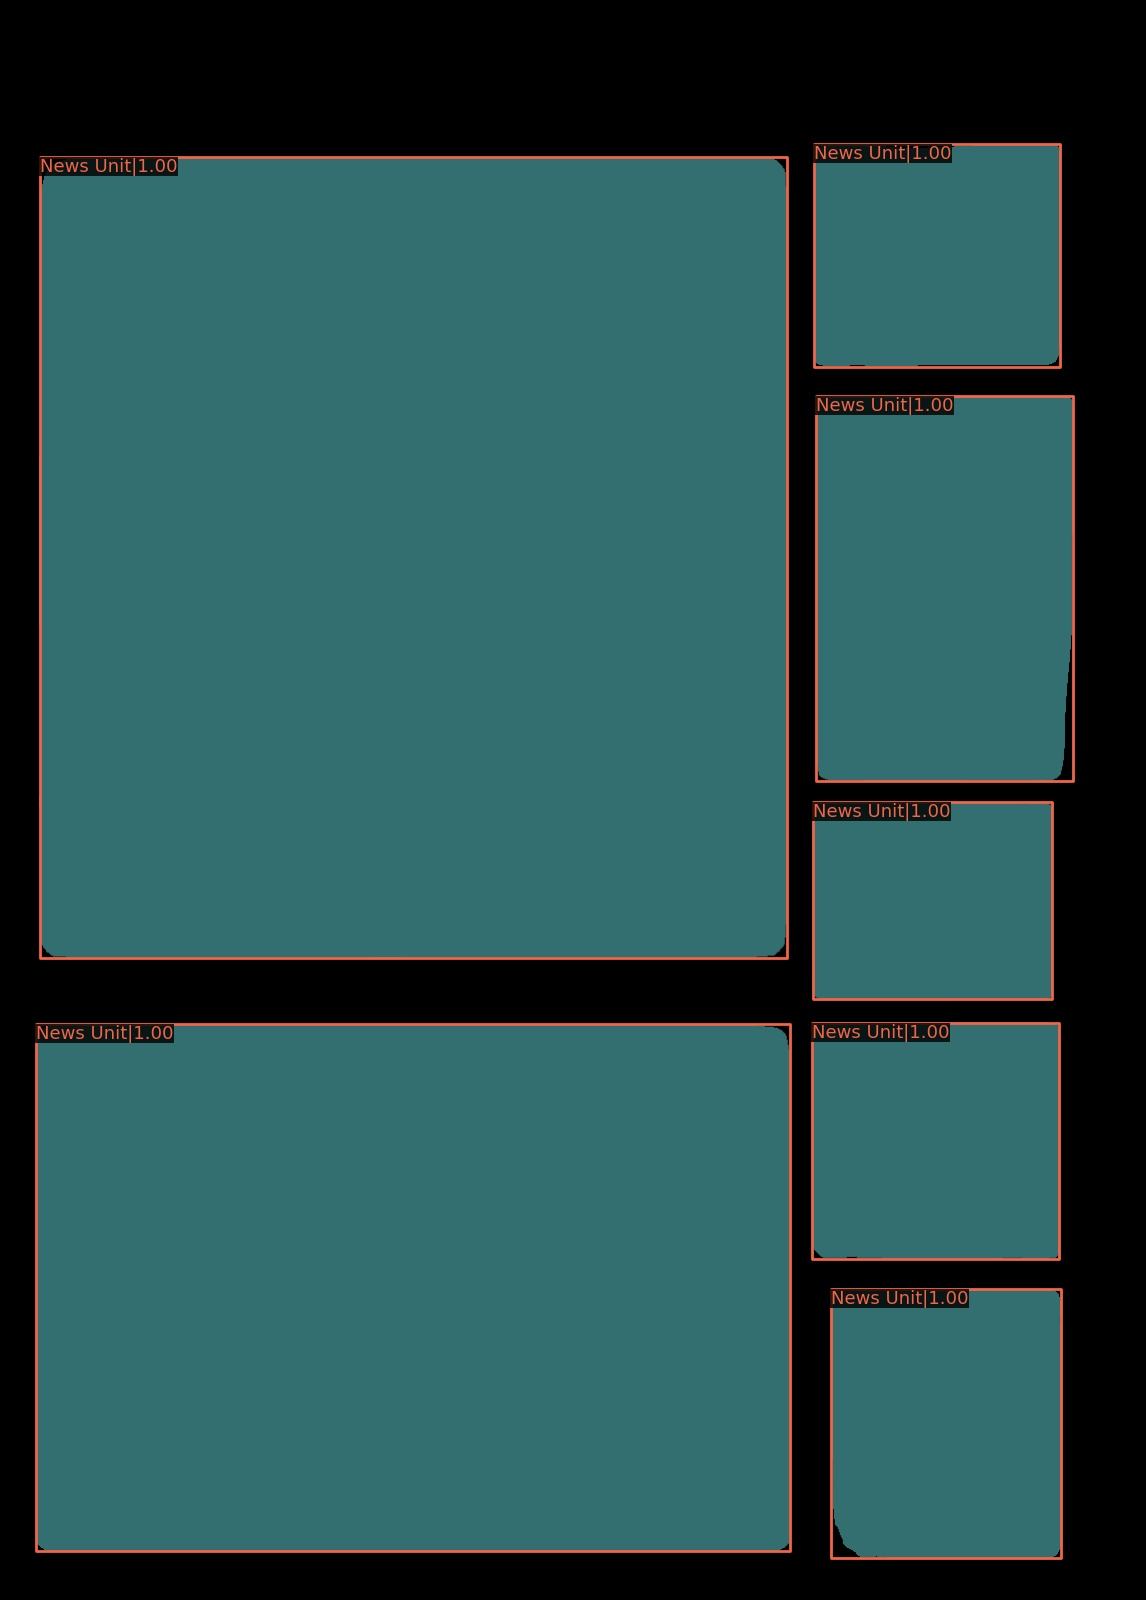
\includegraphics[width=0.99\linewidth, clip=true, trim = 0mm 0mm 0mm 0mm]{figures/labels-vanilla-0.75/AVThDFz.jpg}
  \caption{Model prediction}
\end{subfigure}
\caption{A newspaper page consisting of news articles.}
\label{fig:newsarticles}
\end{figure}
\end{frame}
\normalpage

\normalpage
%%%%%%%%%%%%%%%%%%%%%%%%%%%%%%%%%%%%%%%%%%%%%%%%%%%%%%%%%%%%
\begin{frame}
  \frametitle{Why newspaper article segmentation?}

  \begin{block}{Focus on digitization of documents}
    \begin{itemize}
    \item Pages are scanned on an image level
    \item Optical Character Recognition extracts boxes of text
    \item Document layout analysis: Determining reading order, meaningful article segmentation remains a challenge
    \item Meaningful segments could enable e.g. search on article level, instead of page level.
    \end{itemize}
  \end{block}

\end{frame}
\normalpage


%%%%%%%%%%%%%%%%%%%%%%%%%%%%%%%%%%%%%%%%%%%%%%%%%%%%%%%%%%%%
%\begin{frame}
%\begin{figure}
%\centering
%\begin{subfigure}{.5\textwidth}
%  \centering
%  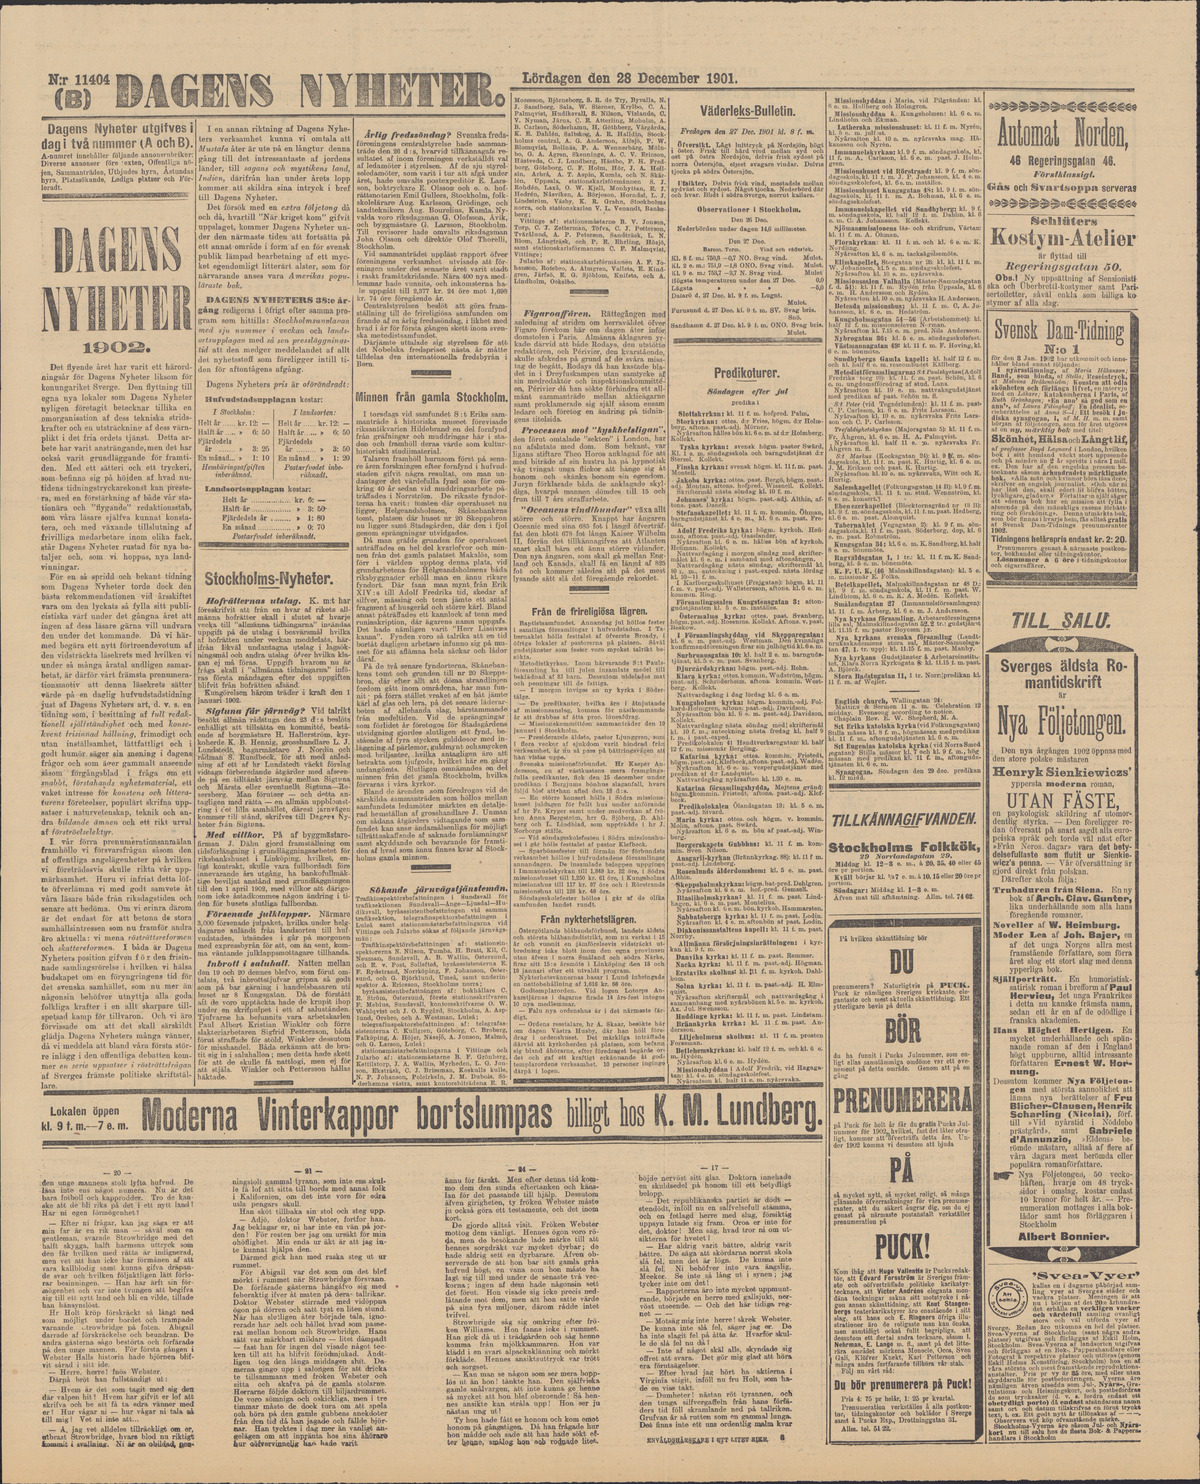
\includegraphics[max size={0.95\textwidth}{0.95\textheight}]{figures/1901.jpg}
%  \caption{A newspaper page from 1901.}
%  \label{fig:raw1901}
%\end{subfigure}%
%\begin{subfigure}{.5\textwidth}
%  \centering
%  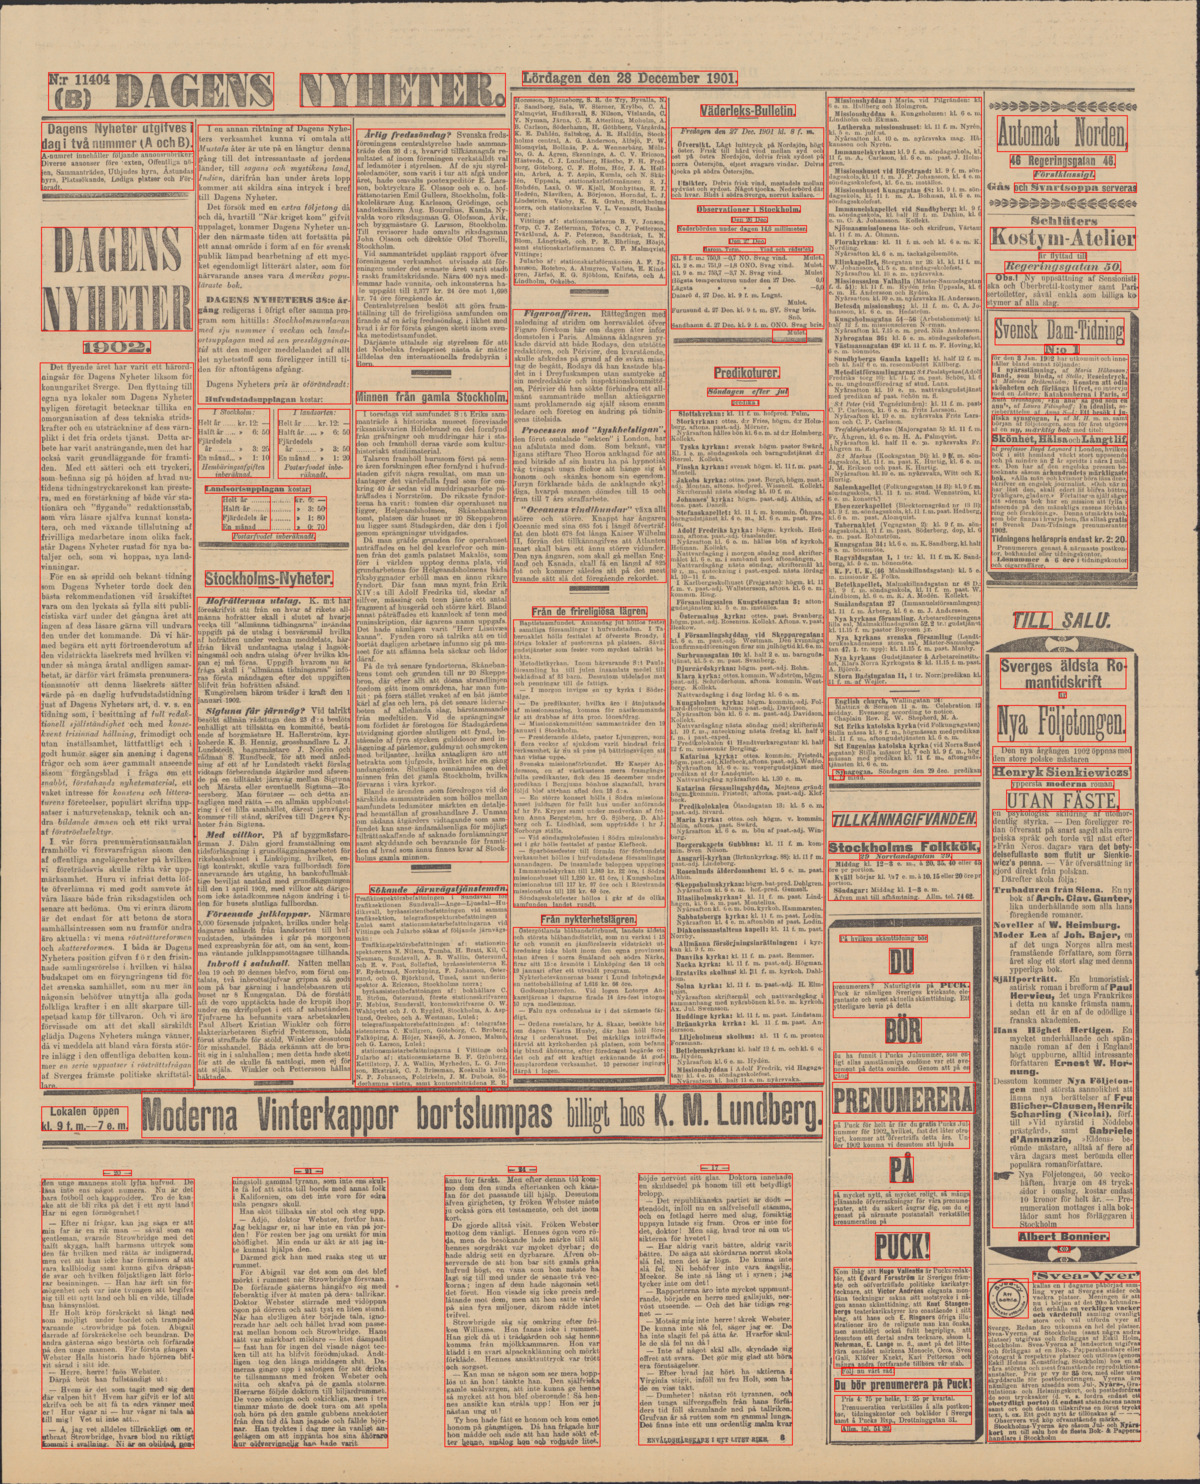
\includegraphics[max size={0.95\textwidth}{0.95\textheight}]{figures/1901-ocr.jpg}
%  \caption{OCR bounding boxes visualized in red.}
%  \label{fig:ocr1901}
%\end{subfigure}
%\label{fig:1901}
%\end{figure}

%\end{frame}
%\normalpage


%%%%%%%%%%%%%%%%%%%%%%%%%%%%%%%%%%%%%%%%%%%%%%%%%%%%%%%%%%%%
\begin{frame}
  \frametitle{Problems and goals}

  \begin{Large}
    Problem statement
  \end{Large}

  \begin{small}
  How well can neural networks, developed for object detection and
segmentation of real-world objects, perform in the domain of news article
segmentation?
  \break
  \end{small}

  \begin{Large}
    Goals 
  \end{Large}


  \begin{small}
    \begin{itemize}
    \item Do multimodal neural network architectures outperform unimodal neural
network architectures, using image and text input as opposed to only
using image input, in the field of instance segmentation?
    \item Is there a difference in how well multimodal neural network architectures
perform in periods of changing typographic design as opposed to
unimodal neural network architectures?
    \end{itemize}
  \end{small}

\end{frame}
\normalpage

%%%%%%%%%%%%%%%%%%%%%%%%%%%%%%%%%%%%%%%%%%%%%%%%%%%%%%%%%%%%
\begin{frame}
  \frametitle{What is Mask R-CNN?}
\begin{figure}
\centering
\begin{subfigure}{0.2\textwidth}
  \centering
  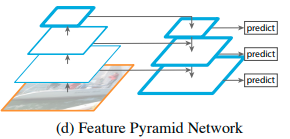
\includegraphics[max size={0.9\textwidth}{0.9\textheight}]{figures/fpnonly.png}
  \label{fig:fpnonly}
\end{subfigure}%
\begin{subfigure}{0.8\textwidth}
  \centering
  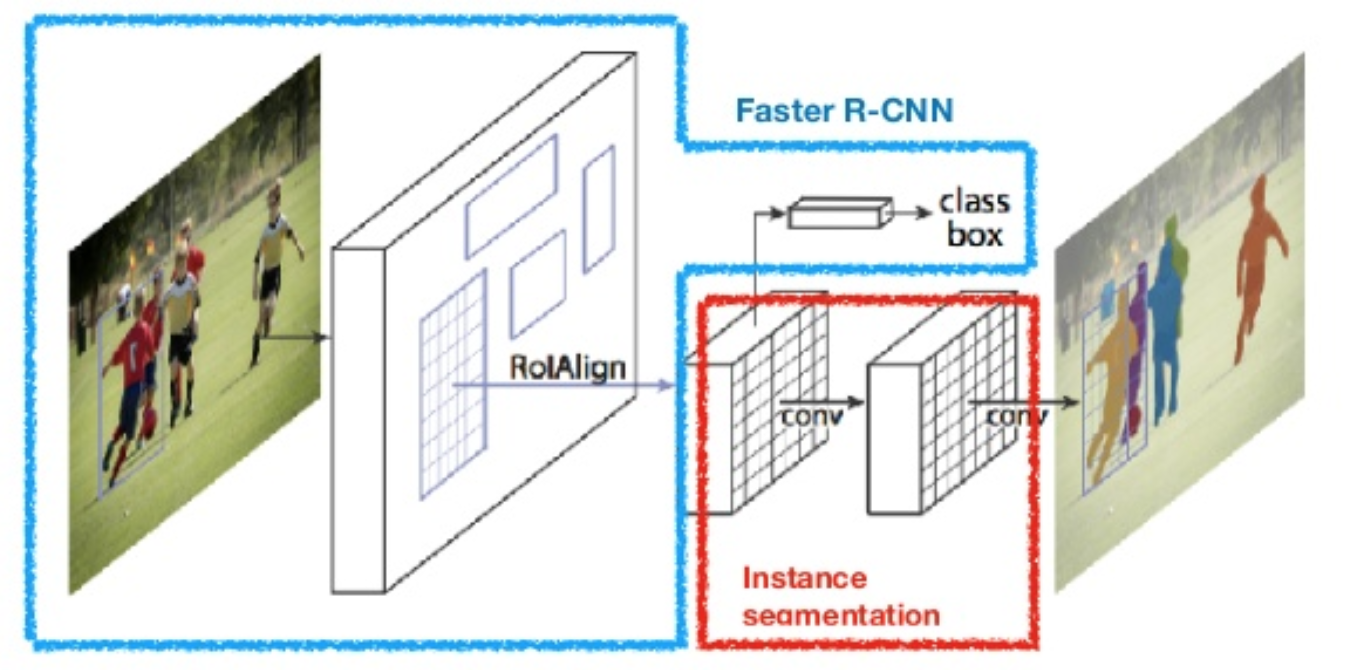
\includegraphics[max size={0.9\textwidth}{0.9\textheight}]{figures/mask-rcnn.png}
  \label{fig:submaskrcnn}
  %https://www.researchgate.net/publication/351426881_Objective_comparison_of_relief_visualization_techniques_with_deep_CNN_for_archaeology
\end{subfigure}%
\label{fig:maskrcnn}
  \caption{Mask R-CNN architecture. [Guyot et al 2021]}
\end{figure}
\end{frame}
\normalpage



%%%%%%%%%%%%%%%%%%%%%%%%%%%%%%%%%%%%%%%%%%%%%%%%%%%%%%%%%%%%
\begin{frame}
  \frametitle{How do we combine the visual and textual modalities?}
\begin{tikzpicture}

    \tikzcuboid{%
        shiftx=12cm,%
        shifty=8cm,%
        scale=0.6,%
        rotation=0,%
        densityx=2,%
        densityy=1,%
        densityz=1,%
        dimx=1,%
        dimy=6,%
        dimz=6,%
        linefront=red!25!white,%
        linetop=red!50!white,%
        lineright=red!25!black,%
        fillfront=red!25!white,%
        filltop=red!50!white,%
        fillright=red!75!white,%
        emphedge=Y,%
        emphstyle=very thick,
    }
    \tikzcuboid{%
        shiftx=14cm,%
        shifty=8cm,%
        scale=0.6,%
        rotation=0,%
        densityx=2,%
        densityy=1,%
        densityz=1,%
        dimx=1,%
        dimy=6,%
        dimz=6,%
        linefront=green!25!white,%
        linetop=green!50!white,%
        lineright=green!25!black,%
        fillfront=green!25!white,%
        filltop=green!50!white,%
        fillright=green!75!white,%
        emphedge=Y,%
        emphstyle=very thick,
    }

    \tikzcuboid{%
        shiftx=16cm,%
        shifty=8cm,%
        scale=0.6,%
        rotation=0,%
        densityx=2,%
        densityy=1,%
        densityz=1,%
        dimx=1,%
        dimy=6,%
        dimz=6,%
        linefront=blue!25!white,%
        linetop=blue!50!white,%
        lineright=blue!25!black,%
        fillfront=blue!25!white,%
        filltop=blue!50!white,%
        fillright=blue!75!white,%
        emphedge=Y,%
        emphstyle=very thick,
    }

    \tikzcuboid{%
        shiftx=18cm,%
        shifty=8cm,%
        scale=0.6,%
        rotation=0,%
        densityx=2,%
        densityy=1,%
        densityz=1,%
        dimx=1,%
        dimy=6,%
        dimz=6,%
        linefront=black!25!white,%
        linetop=black!50!white,%
        lineright=black!25!black,%
        fillfront=black!25!white,%
        filltop=black!50!white,%
        fillright=black!75!white,%
        emphedge=Y,%
        emphstyle=very thick,
    }

    \tikzcuboid{%
        shiftx=20cm,%
        shifty=8cm,%
        scale=0.6,%
        rotation=0,%
        densityx=2,%
        densityy=1,%
        densityz=1,%
        dimx=1,%
        dimy=6,%
        dimz=6,%
        linefront=black!25!white,%
        linetop=black!50!white,%
        lineright=black!25!black,%
        fillfront=black!25!white,%
        filltop=black!50!white,%
        fillright=black!75!white,%
        emphedge=Y,%
        emphstyle=very thick,
    }

    \tikzcuboid{%
        shiftx=22cm,%
        shifty=8cm,%
        scale=0.6,%
        rotation=0,%
        densityx=2,%
        densityy=1,%
        densityz=1,%
        dimx=1,%
        dimy=6,%
        dimz=6,%
        linefront=black!25!white,%
        linetop=black!50!white,%
        lineright=black!25!black,%
        fillfront=black!25!white,%
        filltop=black!50!white,%
        fillright=black!75!white,%
        emphedge=Y,%
        emphstyle=very thick,
    }
\end{tikzpicture}
\begin{small}

3 native RGB channels + 3 text embedding channels
\end{small}
\end{frame}
\normalpage

%%%%%%%%%%%%%%%%%%%%%%%%%%%%%%%%%%%%%%%%%%%%%%%%%%%%%%%%%%%%
\begin{frame}
  \frametitle{Sentence transformers used in this thesis}
\begin{table}[H]
  \begin{center}
    \caption{Sentence transformers}
    \label{tab:modeldimensions}
    \begin{tabular}{l|l}
    \textbf{Model name} & \textbf{Dimensions}  \\
    \hline
    all-mpnet-base-v2 & 384 \\    \hline
    all-MiniLM-L6-v2 & 384 \\    \hline
    multi-qa-mpnet-base-dot-v1 & 384 \\    \hline
    all-distilroberta-v1 & 384 \\    \hline
    KBLab/sentence-bert-swedish-cased & 768 \\    \hline
    KB/bert-base-swedish-cased & 768 \\    \hline
    \end{tabular}
  \end{center}
\end{table}
\end{frame}

\normalpage


%%%%%%%%%%%%%%%%%%%%%%%%%%%%%%%%%%%%%%%%%%%%%%%%%%%%%%%%%%%%
\begin{frame}
  \frametitle{What is (Sentence-) BERT?}
\begin{figure}
\centering
\begin{subfigure}{0.9\textwidth}
  \centering
  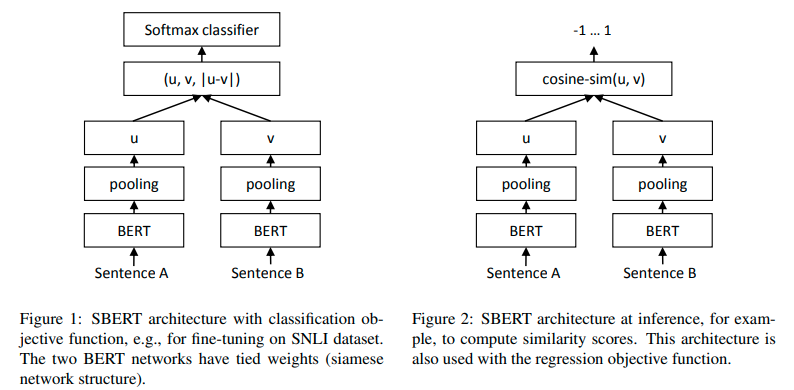
\includegraphics[max size={0.9\textwidth}{0.9\textheight}]{figures/SBERT.png}
  \label{fig:submscoco}
\end{subfigure}%
\label{fig:sbert}
  \caption{Sentence BERT extension of the original BERT. [Reimers et al 2019]}
\end{figure}


\end{frame}
\normalpage

% source for cuboids https://tex.stackexchange.com/a/29882
%%%%%%%%%%%%%%%%%%%%%%%%%%%%%%%%%%%%%%%%%%%%%%%%%%%%%%%%%%%%
\begin{frame}
  \frametitle{Datasets created in this thesis}

\begin{tikzpicture}
 
\node[rectangle,
    draw = lightgray,
    text = black,
    fill = orange!30!,
    minimum width = 6cm, 
    minimum height = 1cm] (r) at (0,0) {\small Train(N=510)};


\node[rectangle,
    draw = lightgray,
    text = black,
    fill = blue!30!,
    minimum width = 2cm, 
    minimum height = 1cm] (r) at (5,0) {\small Test(N=109)};

\node[rectangle,
    draw = lightgray,
    text = black,
    fill = green!30!,
    minimum width = 2cm, 
    minimum height = 1cm] (r) at (8,0) {\small Validation(N=111)};

\node[rectangle,
    draw = white,
    text = black,
    fill = white!30!,
    minimum width = 2cm, 
    minimum height = 1cm] (r) at (11,0) {\small DN 2010-2020};


\node[rectangle,
    draw = lightgray,
    text = black,
    fill = blue!30!,
    minimum width = 2cm, 
    minimum height = 1cm] (r) at (5,-1) {\small Test(N=195)};


\node[rectangle,
    draw = white,
    text = black,
    fill = white!30!,
    minimum width = 2cm, 
    minimum height = 1cm] (r) at (11,-1) {\small DN SvD 2001-2004};

\node[rectangle,
    draw = lightgray,
    text = black,
    fill = blue!30!,
    minimum width = 2cm, 
    minimum height = 1cm] (r) at (5,-2) {\small Test(N=200)};


\node[rectangle,
    draw = white,
    text = black,
    fill = white!30!,
    minimum width = 2cm, 
    minimum height = 1cm] (r) at (11,-2) {AB EX 2001-2004};
\end{tikzpicture}

\begin{small}
Morning newspapers: DN = Dagens Nyheter, SvD = Svenska Dagbladet

Evening newspapers: AB = Aftonbladet, EX = Expressen


DN 2010-2020 is split (70/15/15) using random sampling.
\end{small}
\end{frame}
\normalpage

%%%%%%%%%%%%%%%%%%%%%%%%%%%%%%%%%%%%%%%%%%%%%%%%%%%%%%%%%%%%
\begin{frame}
  \frametitle{Labeling Strategy}

Classes:
\begin{description}
\item[$\bullet$] News Unit
\item[$\bullet$] Advertisement
\item[$\bullet$] Listing
\item[$\bullet$] Weather
\item[$\bullet$] Death Notice
\item[$\bullet$] Game
\item[$\bullet$] Publication Unit (All of the above as 1 class, for testing class confusion)
\end{description}

Caveats:
\begin{description}
\item[$\bullet$] Rectangles to polygons
\item[$\bullet$] Spatial blocking of content
\item[$\bullet$] Per page annotations (Implied content)
\end{description}
\end{frame}
\normalpage


%%%%%%%%%%%%%%%%%%%%%%%%%%%%%%%%%%%%%%%%%%%%%%%%%%%%%%%%%%%%
\begin{frame}
  \frametitle{Experiments}

\begin{description}
\item[$\bullet$] Unimodal vs multimodal (Image vs image + text)
\item[$\bullet$] Impact of class labels (6 classes vs 1 class)
\item[$\bullet$] Impact of dataset size (Random sampling different \% of train data)
\end{description}

\end{frame}
\normalpage


%%%%%%%%%%%%%%%%%%%%%%%%%%%%%%%%%%%%%%%%%%%%%%%%%%%%%%%%%%%%
\begin{frame}
  \frametitle{Performance Metrics}
\begin{equation}
    IoU = \frac{Area \: Overlap}{Area \: Union}
    \label{eqn:iou}
\end{equation}

A prediction is considered positive when above a certain threshold $\tau \in [0,1]$ of IoU.
\begin{equation}
    Precision @ \tau = P@\tau = \frac{TP}{(TP + FP)}
    \label{eqn:precision}
\end{equation}

mean Average Precision:
\begin{equation}
mAP = \frac{1}{N} \sum_{i=1}^{N} AP_i
    \label{eqn:map}
\end{equation}

mean Average Precision at different IoU thresholds:

\begin{equation}
mAP^{50} = mAP^{(IoU=0.5)}
    \label{eqn:map}
\end{equation}

Metrics are reported on the segmentation mask (m) and bounding box (bb) respectively.

\end{frame}
\normalpage


%%%%%%%%%%%%%%%%%%%%%%%%%%%%%%%%%%%%%%%%%%%%%%%%%%%%%%%%%%%%
\begin{frame}
  \frametitle{Major results}
  Impact of dataset size - Varying a \% of the training data using random sampling. Each experiment was repeated 5 times.

  \begin{table}[H]
  \begin{center}
    \caption{Gradually increasing dataset size - 6 classes - In-domain test set}
    \label{tab:dsizeallcinset}
    \resizebox{\columnwidth}{!}{
    \begin{tabular}{l|l|l|l|l|l|l|l}
    \textbf{\% Train} & \textbf{$mAP_m$} & \textbf{$mAP_m^{50}$} & \textbf{$mAP_m^{75}$} & \textbf{$mAP_{bb}$} & \textbf{$mAP_{bb}^{50}$} & \textbf{$mAP_{bb}^{75}$} & \textbf{$\sigma$} \\
    \hline
    25\% & 0.723 & 0.848 & 0.790 & 0.688 & 0.847 & 0.781 & 0.027 \\    \hline
    50\% & 0.883 & 0.964 & 0.945 & 0.850 & 0.965 & 0.943 & 0.003 \\    \hline
    75\% & \textbf{0.939} & \textbf{0.989} & \textbf{0.981} & \textbf{0.927} & \textbf{0.989} & \textbf{0.980} & 0.004 \\    \hline
    90\% & 0.934 & 0.976 & 0.963 & 0.921 & 0.975 & 0.962 & 0.006 \\    \hline
    100\% & 0.901 & 0.960 & 0.935 & 0.895 & 0.960 & 0.934 & 0.005 \\    \hline

    \end{tabular}}
  \end{center}
\end{table}
The standard deviation $\sigma$ denotes the average of the standard deviations of each cell in the
row. All results in this table derive from the model resnet-50-FPN. All prediction visualizations in this presentation are produced by the top scoring model (75\%).

\end{frame}
\normalpage

%%%%%%%%%%%%%%%%%%%%%%%%%%%%%%%%%%%%%%%%%%%%%%%%%%%%%%%%%%%%
\begin{frame}
  \frametitle{Major Results 2}
\begin{table}[H]
  \begin{center}
    \caption{Top 5 results - 6 classes - In-domain test set - 100\% of train data}
    \label{tab:top5allcinset}
    \resizebox{\columnwidth}{!}{
    \begin{tabular}{l|l|l|l|l|l|l} %
    \textbf{Final name} & \textbf{$mAP_m$} & \textbf{$mAP_m^{50}$} & \textbf{$mAP_m^{75}$} & \textbf{$mAP_{bb}$} & \textbf{$mAP_{bb}^{50}$} & \textbf{$mAP_{bb}^{75}$} \\
    \hline
x101-32x8d                     & 0.910 & 0.964 & 0.936 & 0.906 & 0.964 & 0.937 \\ \hline
x101-32x4d                     & 0.906 & 0.957 & 0.929 & 0.901 & 0.957 & 0.932 \\ \hline
x101-64x4d                     & 0.903 & 0.954 & 0.934 & 0.893 & 0.954 & 0.934 \\ \hline
r101                           & 0.901 & 0.951 & 0.928 & 0.885 & 0.953 & 0.927 \\ \hline
x101-64x4d-all-mpnet           & 0.881 & 0.952 & 0.927 & 0.868 & 0.954 & 0.929 \\ \hline
    \end{tabular}}
  \end{center}
\end{table}
\end{frame}
\normalpage

%%%%%%%%%%%%%%%%%%%%%%%%%%%%%%%%%%%%%%%%%%%%%%%%%%%%%%%%%%%%
\begin{frame}
  \frametitle{Major Results 3}

  Multimodal models tended to outperform unimodal models on the out-of-domain test set when all classes are set to the same class: Publication Unit.

\begin{table}[H]
  \begin{center}
    \caption{Top 5 results - 1 class - Out-set}
    \label{tab:top5onecoutset}
    \resizebox{\columnwidth}{!}{
    \begin{tabular}{l|l|l|l|l|l|l}
    \textbf{Final name} & \textbf{$mAP_m$} & \textbf{$mAP_m^{50}$} & \textbf{$mAP_m^{75}$} & \textbf{$mAP_{bb}$} & \textbf{$mAP_{bb}^{50}$} & \textbf{$mAP_{bb}^{75}$} \\
    \hline
r50-MiniLM-1c                  & 0.465 & 0.622 & 0.490 & 0.458 & 0.622 & 0.488 \\ \hline
r50-all-mpnet-1c               & 0.455 & 0.612 & 0.480 & 0.449 & 0.611 & 0.483 \\ \hline
x101-64x4d-all-mpnet-1c        & 0.447 & 0.588 & 0.474 & 0.441 & 0.585 & 0.474 \\ \hline
r50-1c                         & 0.438 & 0.560 & 0.460 & 0.432 & 0.556 & 0.462 \\ \hline
x101-all-mpnet-1c              & 0.433 & 0.564 & 0.459 & 0.426 & 0.564 & 0.456 \\ \hline
    \end{tabular}}
  \end{center}
\end{table}
\end{frame}
\normalpage

%%%%%%%%%%%%%%%%%%%%%%%%%%%%%%%%%%%%%%%%%%%%%%%%%%%%%%%%%%%%
\begin{frame}
  \frametitle{Minor Results}

\begin{table}[H]
  \begin{center}
    \caption{Top performing class choice}
    \label{tab:beststrat}
    \resizebox{0.4\columnwidth}{!}{
    \begin{tabular}{l|l}
    \textbf{Test set} & \textbf{Number of classes} \\
    \hline
In-set  & 6 classes \\ \hline
Near-set & 1 class \\ \hline
Out-set & 6 classes \\ \hline
    \end{tabular}}
  \end{center}
\end{table}


\end{frame}
\normalpage

%%%%%%%%%%%%%%%%%%%%%%%%%%%%%%%%%%%%%%%%%%%%%%%%%%%%%%%%%%%%
\begin{frame}
  \frametitle{Discussion and conclusion}
\begin{description}
\item[$\bullet$] Higher mAP is generally required in this domain for usefulness (simpler masks)
\item[$\bullet$] Vanilla Mask R-CNN has been shown to perform well on in-domain test sets.
\item[$\bullet$] Increase in error in dataset size experiment can be attributed to small dataset size + more complex examples left out in 75\%, and not represented in test set. The greater the size of the training dataset, the better performance on near- and out-of-domain test sets (for both 6 classes and 1 class).
\item[$\bullet$] 6 classes vs 1 class differs in best performance between in-, near- and out-of-domain test sets.
\item[$\bullet$] We make no claims on the ability to generalize across typologies, but we see a consistent drop in performance proportional to 'distance' in typology and timespan.
\item[$\bullet$] Multimodal performance could be explained by large and sparse dimensions, causing the model to ignore those dimensions. (Future work)
\end{description}

\end{frame}
\normalpage

%%%%%%%%%%%%%%%%%%%%%%%%%%%%%%%%%%%%%%%%%%%%%%%%%%%%%%%%%%%%
\begin{frame}
  \frametitle{Future work}
\begin{description}
\item[$\bullet$] Domain-specific architecture
\item[$\bullet$] Normalization of textual embeddings
\item[$\bullet$] Dimensionality reduction of textual embeddings
\item[$\bullet$] Dataset specific image normalization values and training without pretrained weights.
\item[$\bullet$] Text granularity (sentence level, word level, one hot encoding)
\end{description}

\end{frame}
\normalpage

%%%%%%%%%%%%%%%%%%%%%%%%%%%%%%%%%%%%%%%%%%%%%%%%%%%%%%%%%%%%
\begin{frame}
  \frametitle{Demo}
\begin{description}
\item[$\bullet$] Left: First 3 dimensions of all-mpnet-base-v2 vector representations normalized as RGB colors.
\item[$\bullet$] Right: Labels produced by vanilla Mask R-CNN, trained on 75\% of the training data. Close to ground truth in segmentation mask. (0.939 $mAP_{m}$)
\end{description}

\end{frame}
\normalpage

%%%%%%%%%%%%%%%%%%%%%%%%%%%%%%%%%%%%%%%%%%%%%%%%%%%%%%%%%%%%
\begin{frame}
  \begin{figure}
\centering
\begin{subfigure}{.25\textwidth}
  \centering
  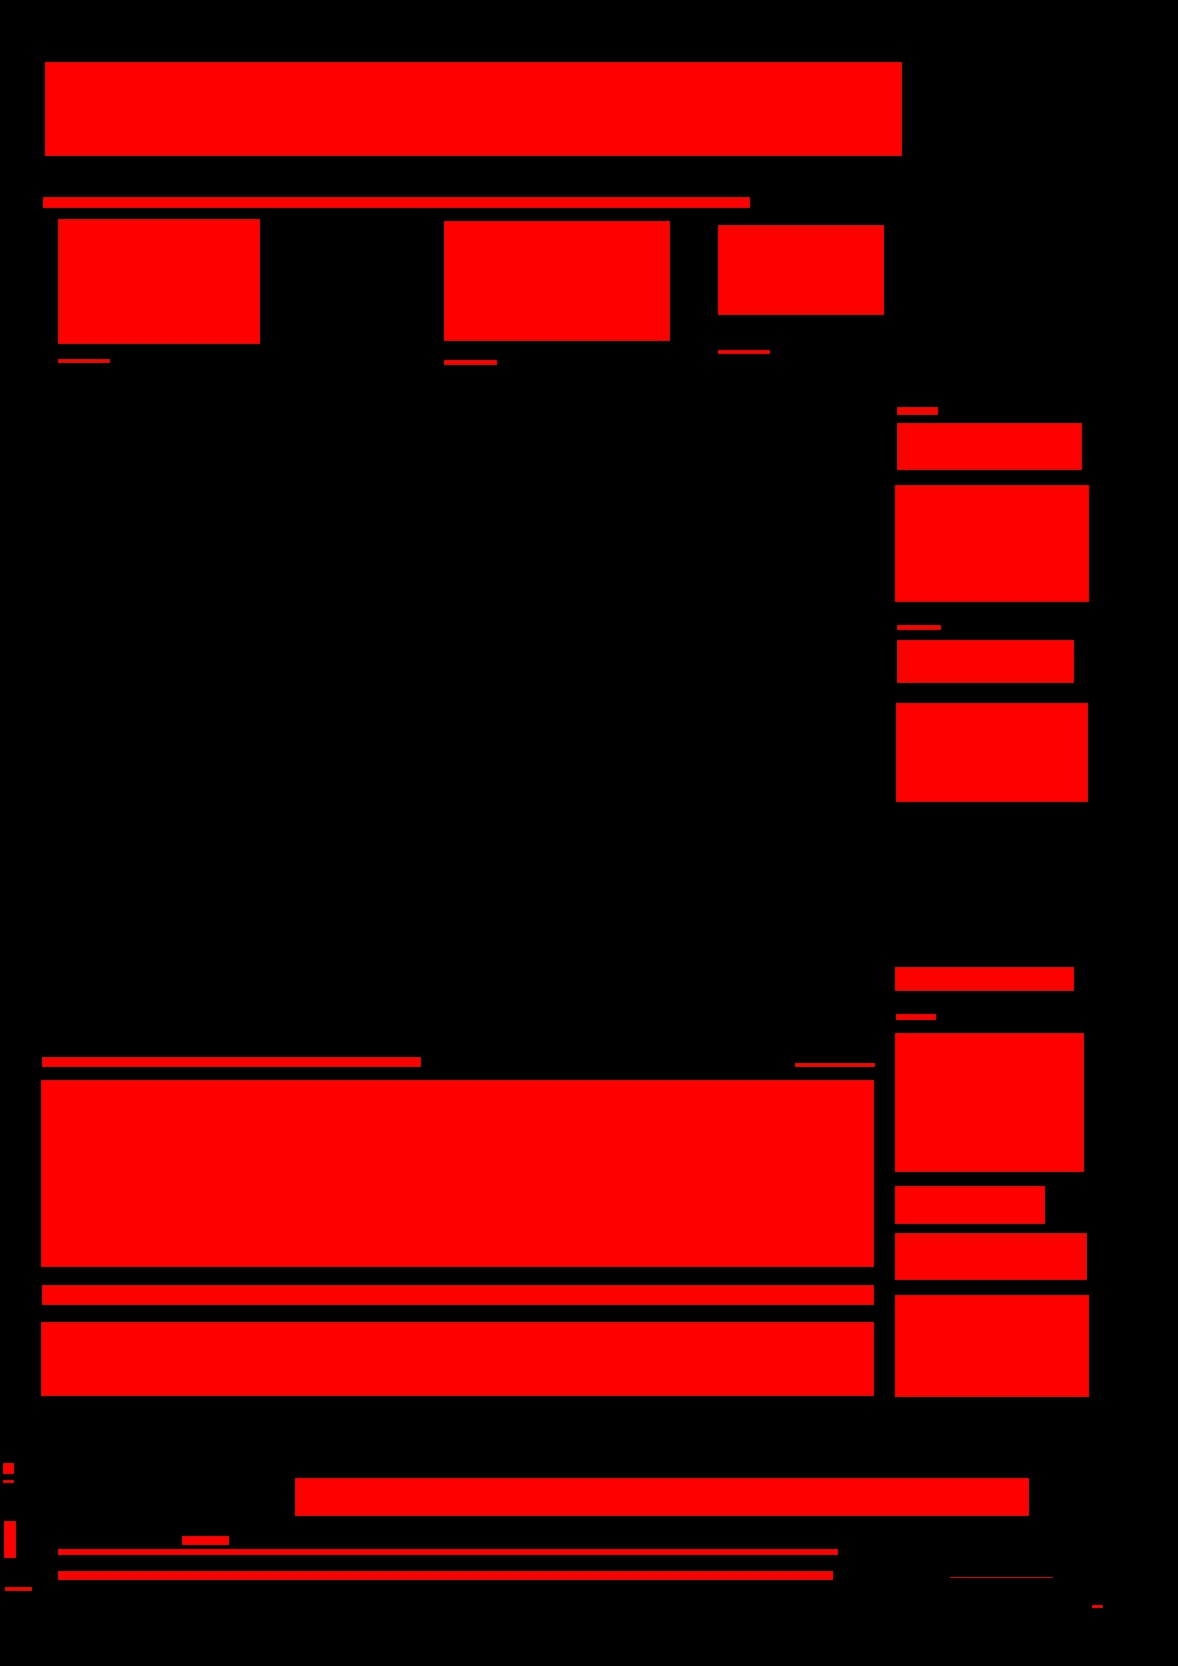
\includegraphics[width=0.99\linewidth, clip=true, trim = 0mm 0mm 0mm 0mm]{figures/ocr/JIefsDa.jpg}
  \caption{OCR}
\end{subfigure}%
\begin{subfigure}{.25\textwidth}
  \centering
  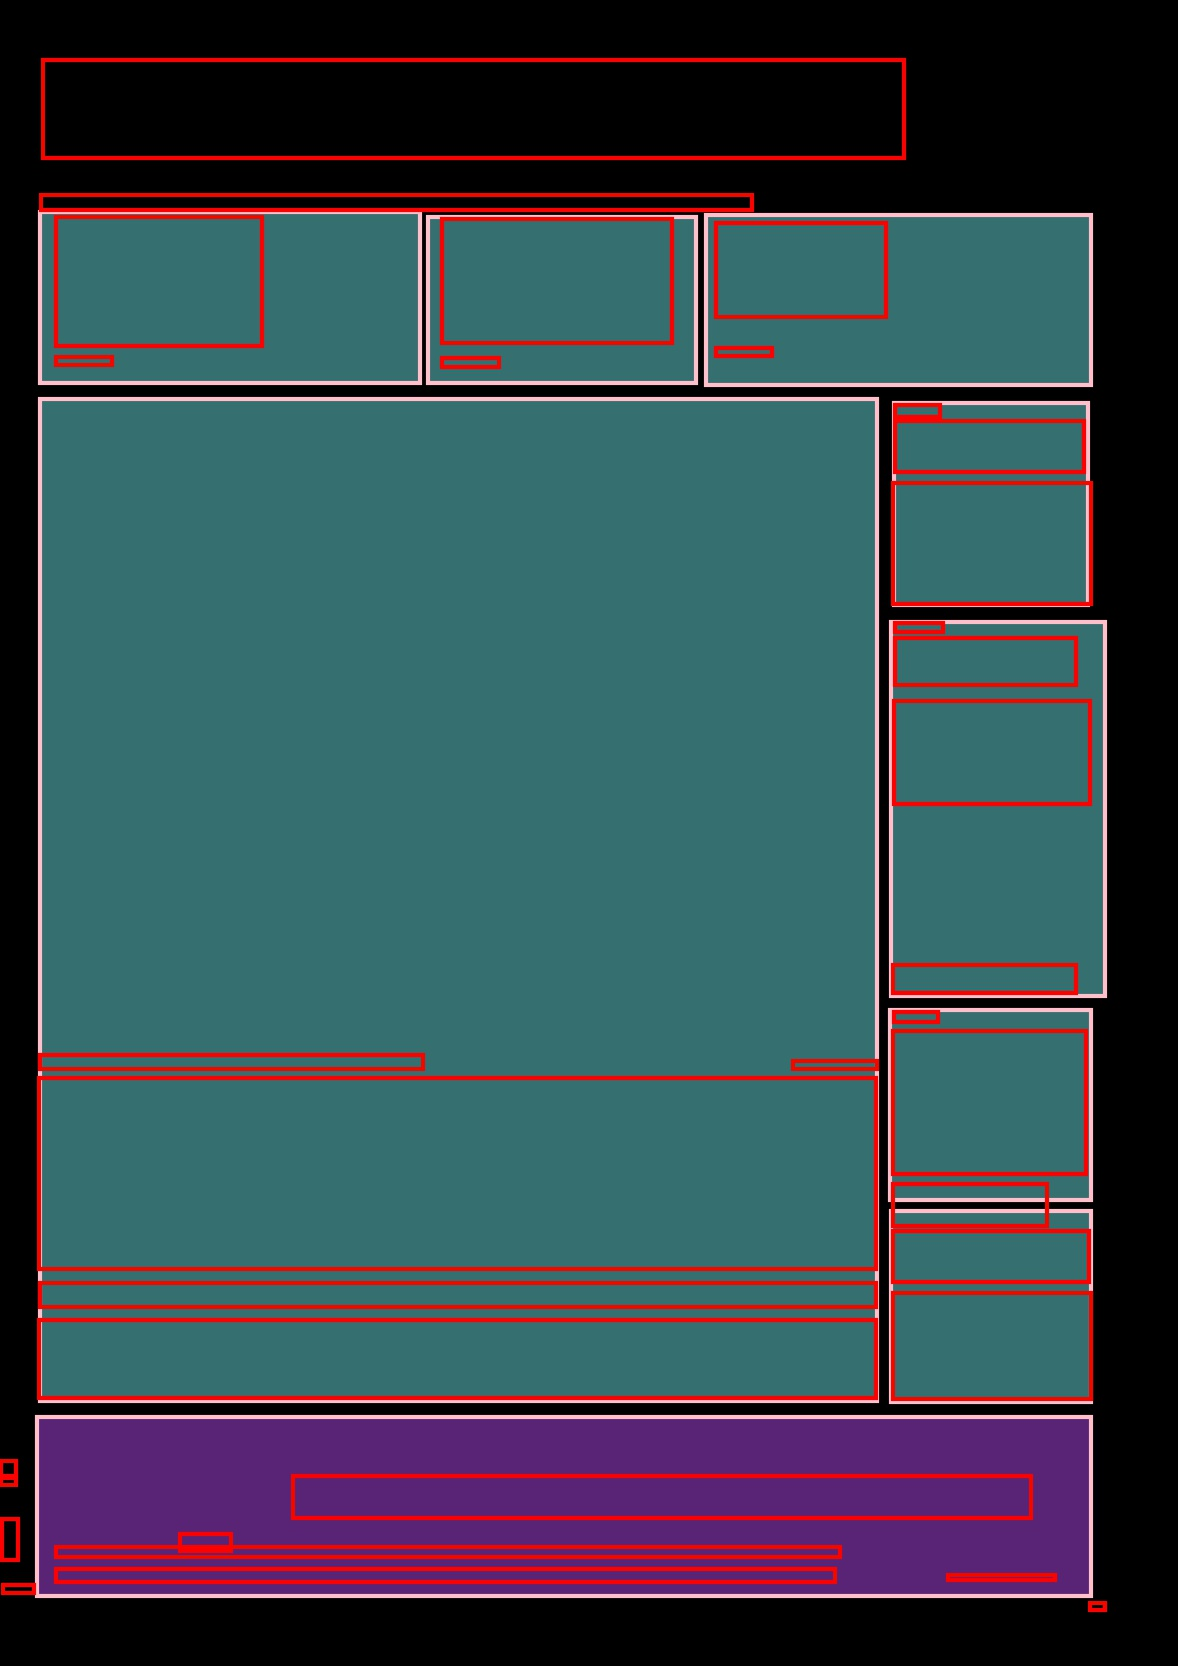
\includegraphics[width=0.99\linewidth, clip=true, trim = 0mm 0mm 0mm 0mm]{figures/ocr_bbox/JIefsDa.jpg}
  \caption{GT Label + OCR}
\end{subfigure}%
\begin{subfigure}{.25\textwidth}
  \centering
  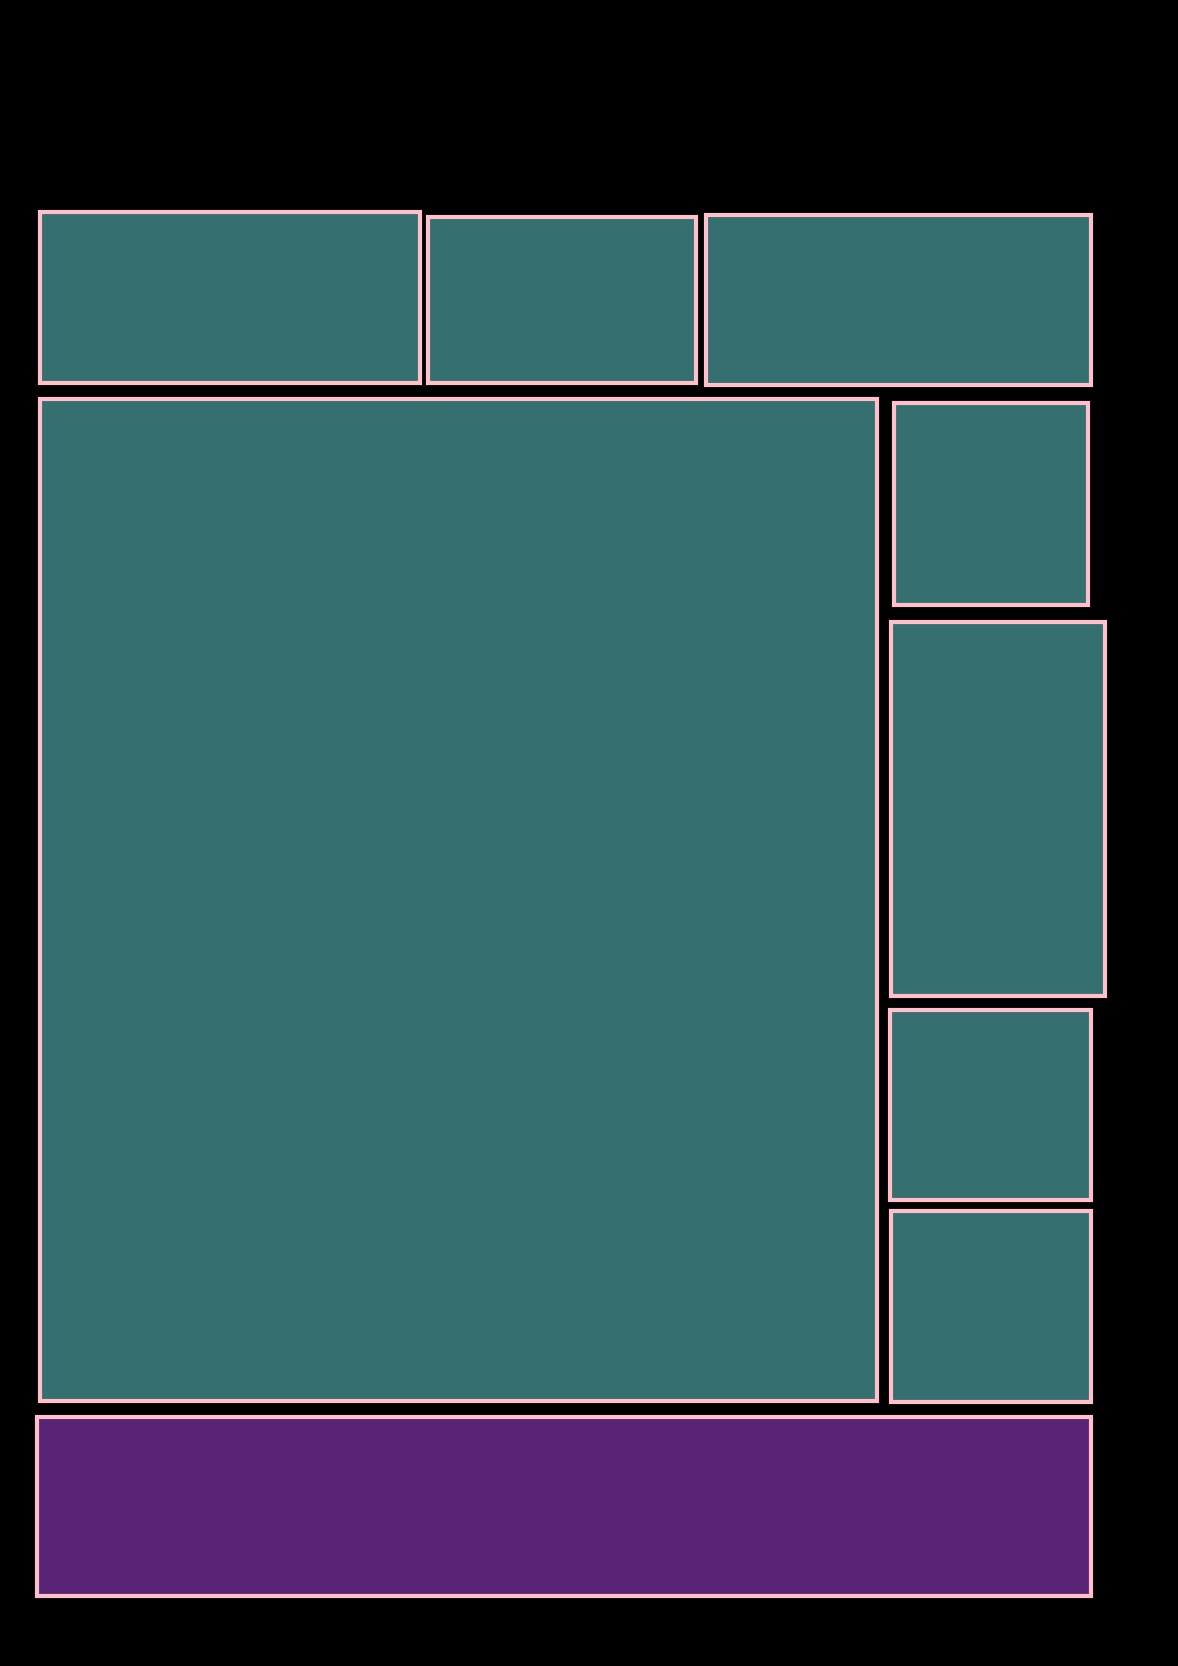
\includegraphics[width=0.99\linewidth, clip=true, trim = 0mm 0mm 0mm 0mm]{figures/bbox/JIefsDa.jpg}
  \caption{GT Label}
\end{subfigure}%
\begin{subfigure}{.25\textwidth}
  \centering
  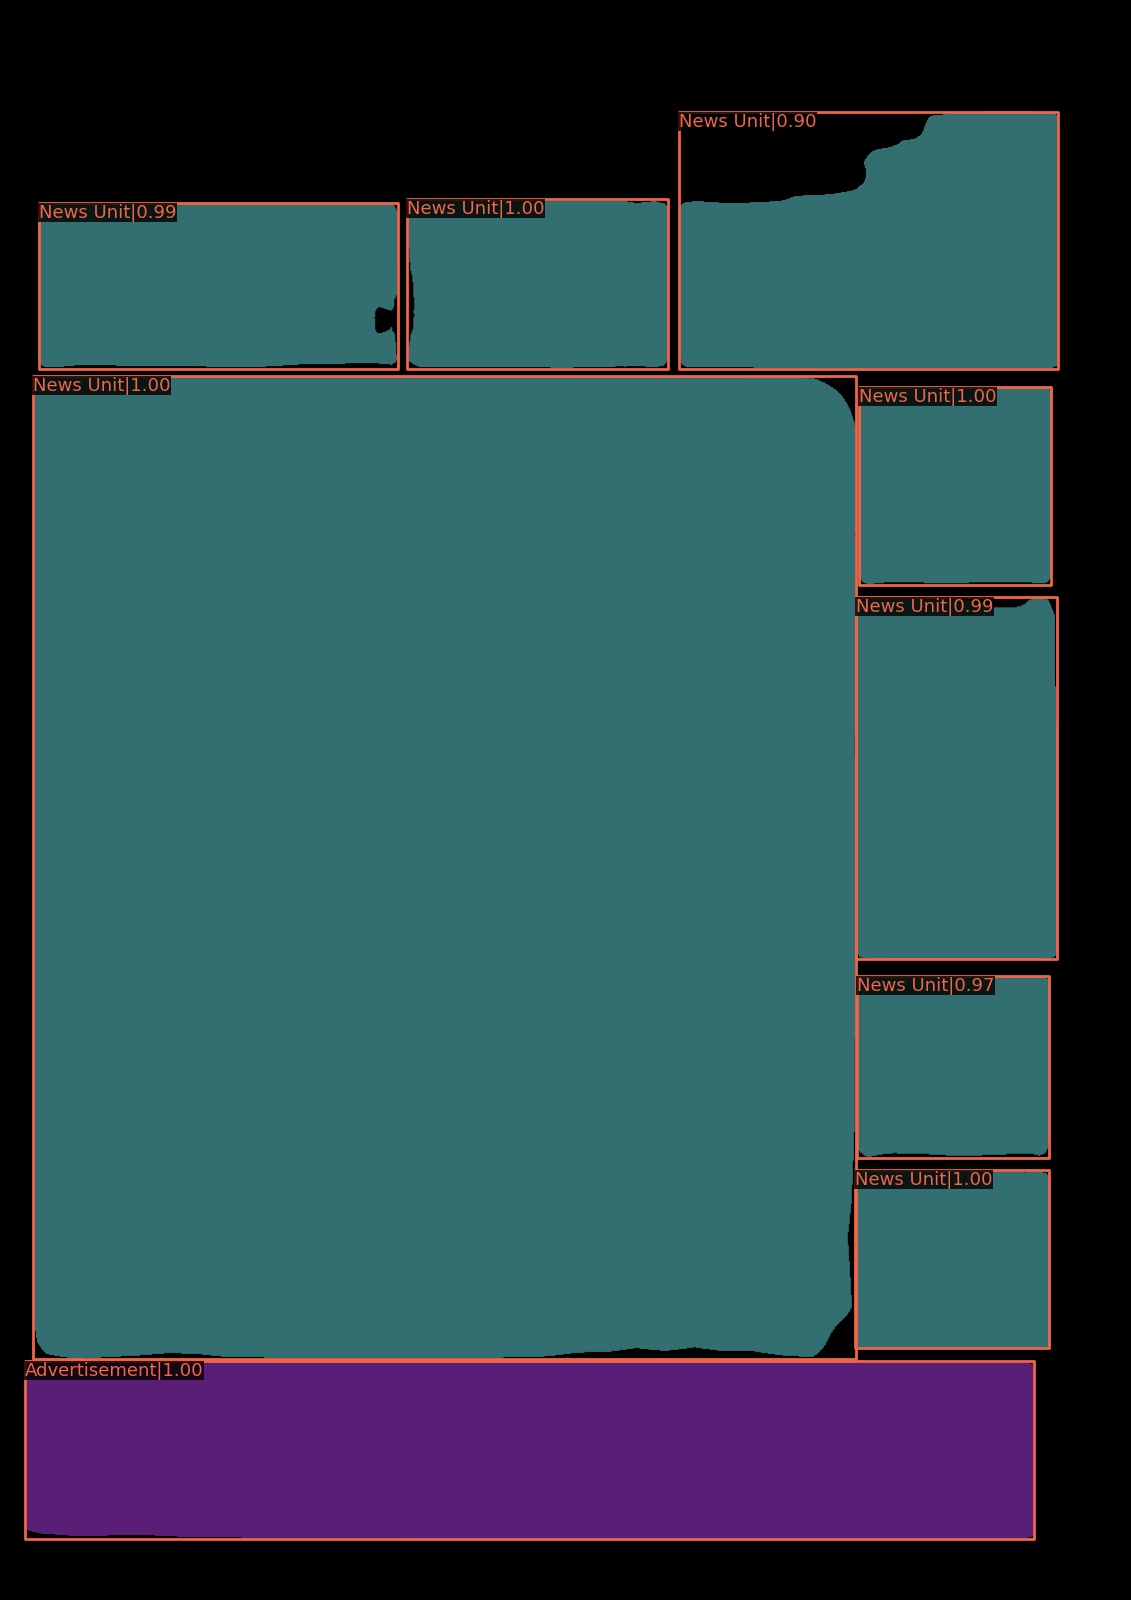
\includegraphics[width=0.99\linewidth, clip=true, trim = 0mm 0mm 0mm 0mm]{figures/labels-vanilla-0.75/JIefsDa.jpg}
  \caption{Model prediction}
\end{subfigure}
\caption{A front page newspaper page from the DN 2010-2020 Test subset.}
\label{fig:front}
\end{figure}

\end{frame}
\normalpage

%%%%%%%%%%%%%%%%%%%%%%%%%%%%%%%%%%%%%%%%%%%%%%%%%%%%%%%%%%%%
\begin{frame}
  \begin{figure}
\centering
\begin{subfigure}{.25\textwidth}
  \centering
  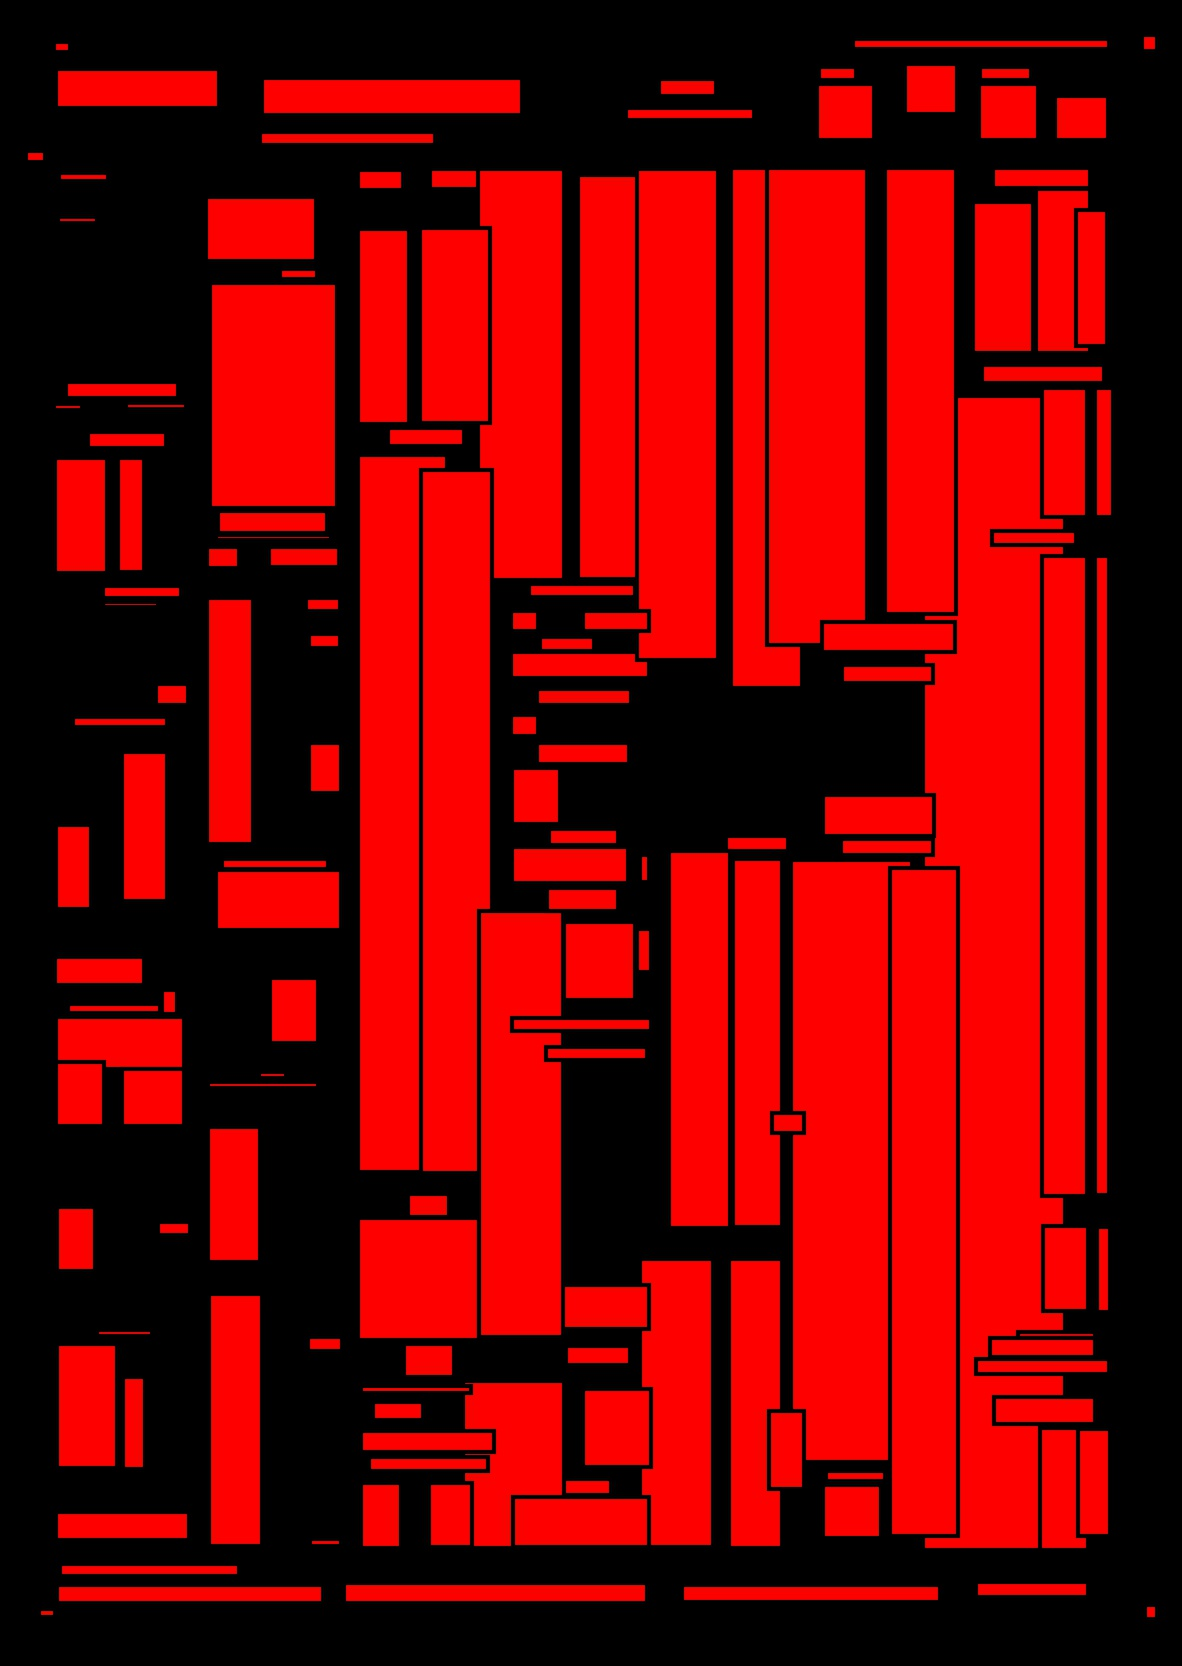
\includegraphics[width=0.99\linewidth, clip=true, trim = 0mm 0mm 0mm 0mm]{figures/ocr/zk6UnuL.jpg}
  \caption{OCR}
\end{subfigure}%
\begin{subfigure}{.25\textwidth}
  \centering
  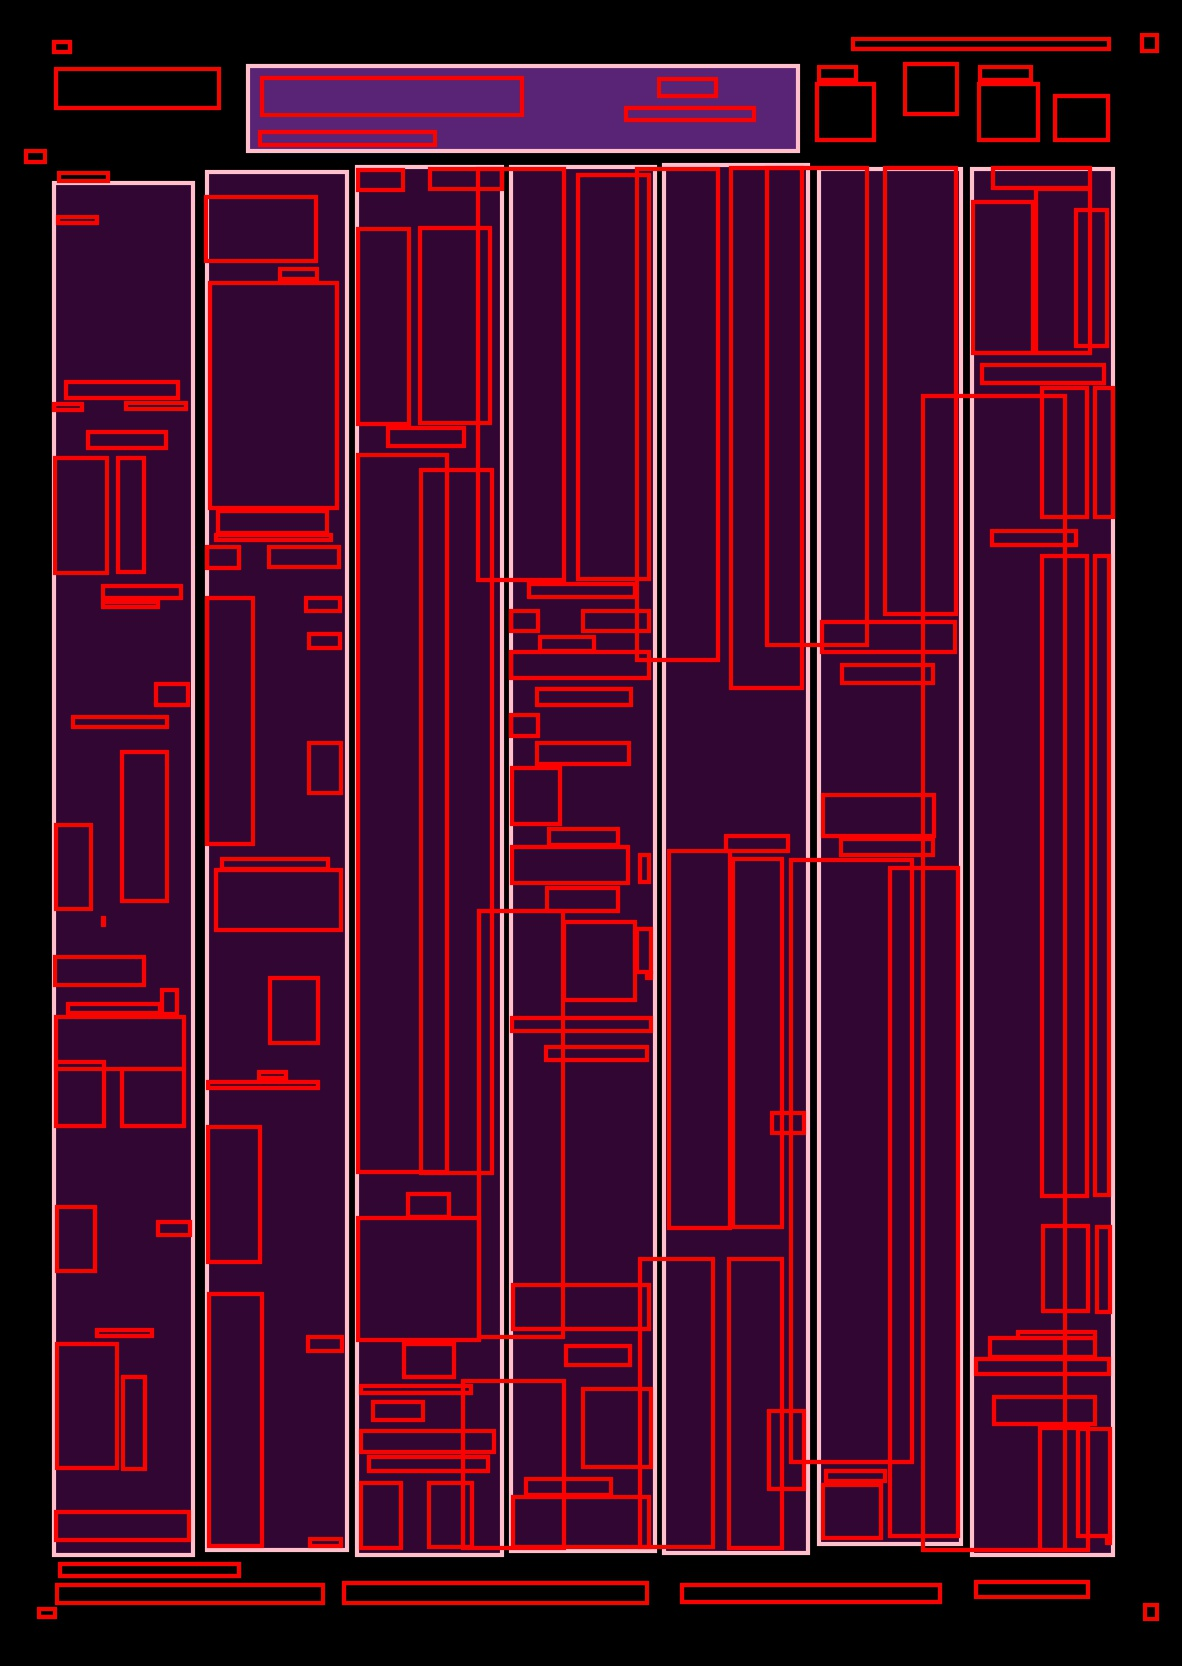
\includegraphics[width=0.99\linewidth, clip=true, trim = 0mm 0mm 0mm 0mm]{figures/ocr_bbox/zk6UnuL.jpg}
  \caption{GT Label + OCR}
\end{subfigure}%
\begin{subfigure}{.25\textwidth}
  \centering
  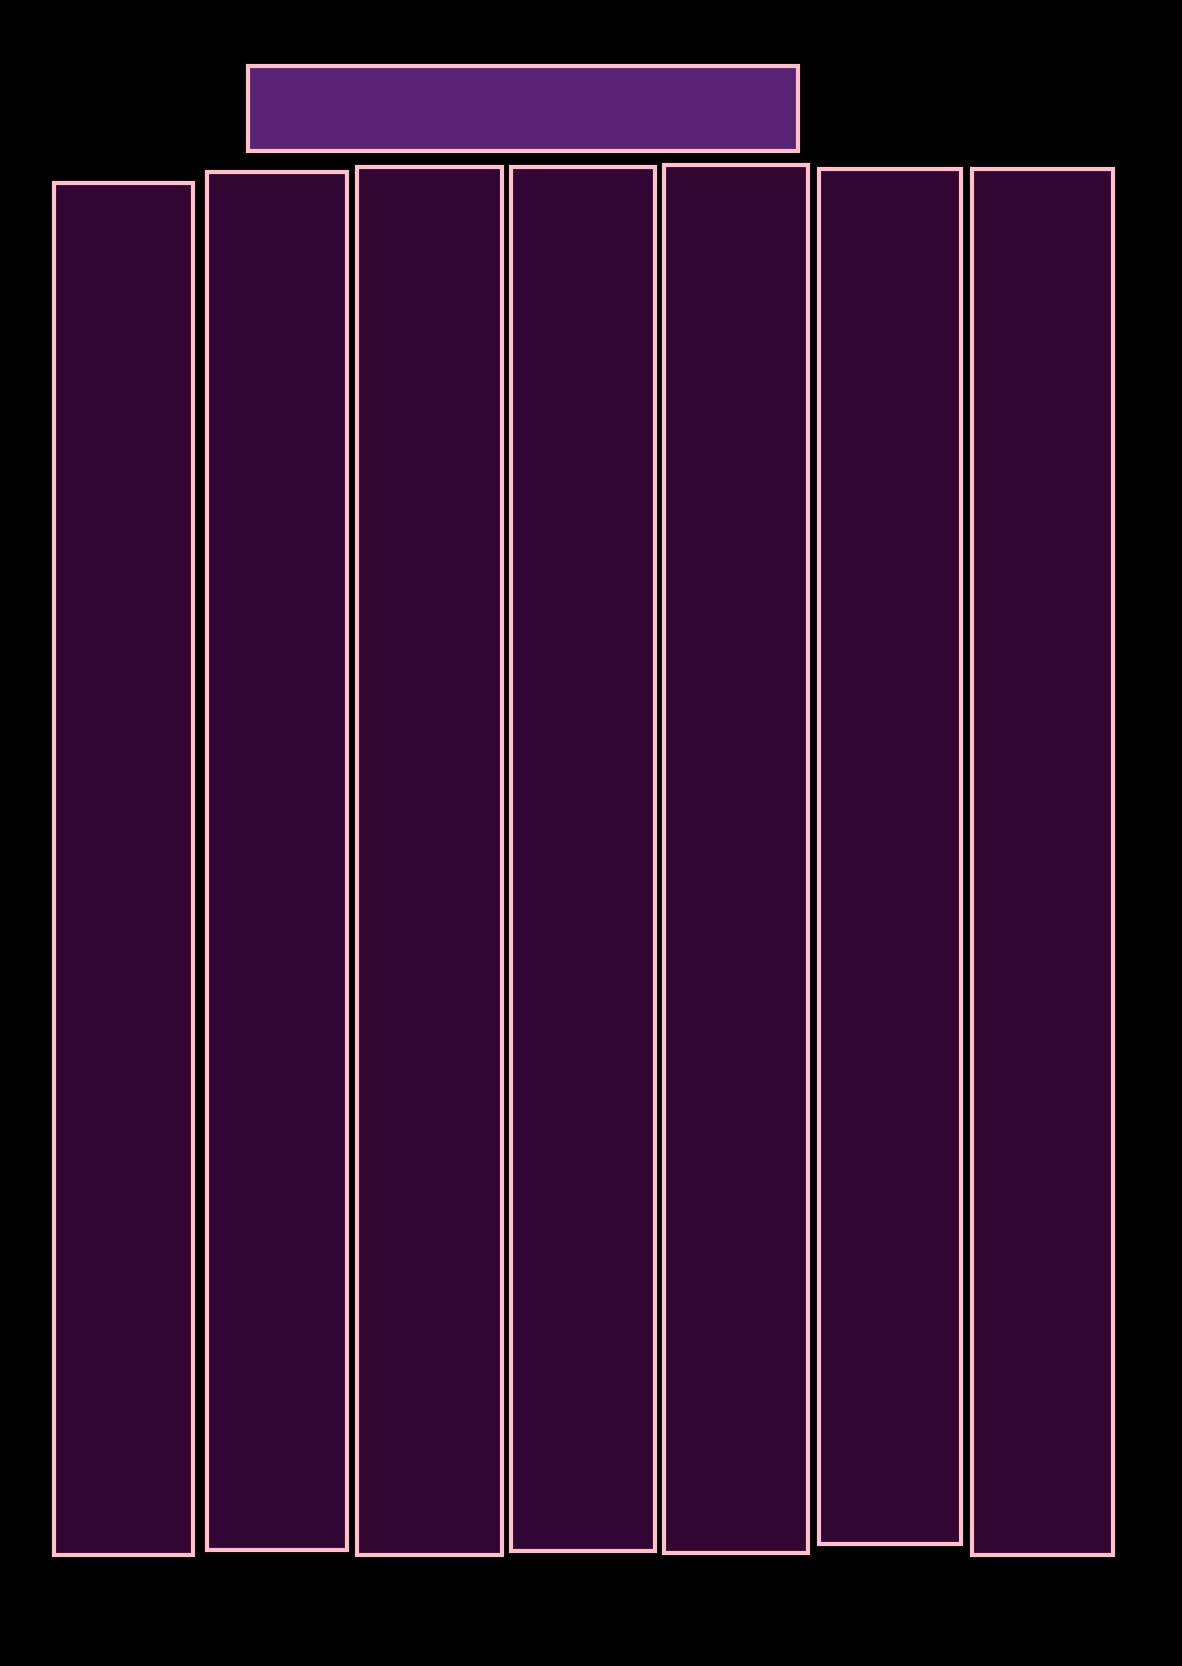
\includegraphics[width=0.99\linewidth, clip=true, trim = 0mm 0mm 0mm 0mm]{figures/bbox/zk6UnuL.jpg}
  \caption{GT Label}
\end{subfigure}%
\begin{subfigure}{.25\textwidth}
  \centering
  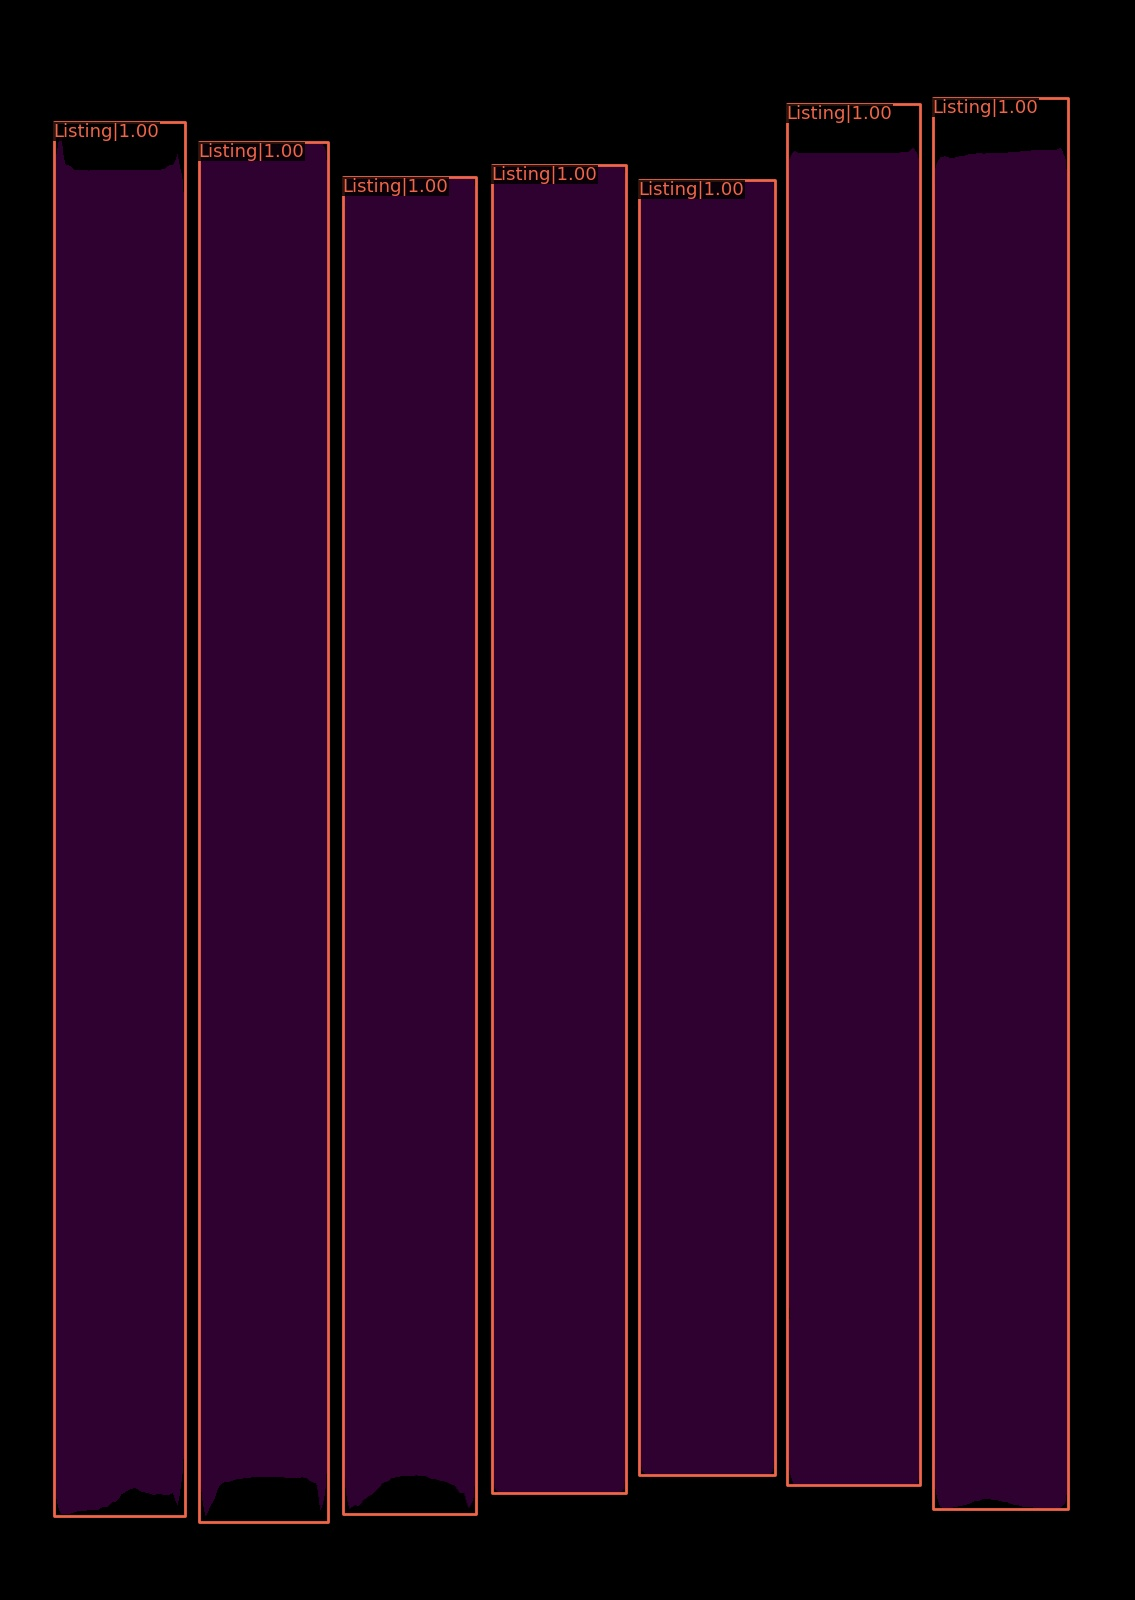
\includegraphics[width=0.99\linewidth, clip=true, trim = 0mm 0mm 0mm 0mm]{figures/labels-vanilla-0.75/zk6UnuL.jpg}
  \caption{Model prediction}
\end{subfigure}
\caption{A newspaper page with listing prices of funds and stocks.}
\label{fig:stocks}
\end{figure}
\end{frame}
\normalpage


%%%%%%%%%%%%%%%%%%%%%%%%%%%%%%%%%%%%%%%%%%%%%%%%%%%%%%%%%%%%
\begin{frame}
  \begin{figure}
\centering
\begin{subfigure}{.25\textwidth}
  \centering
  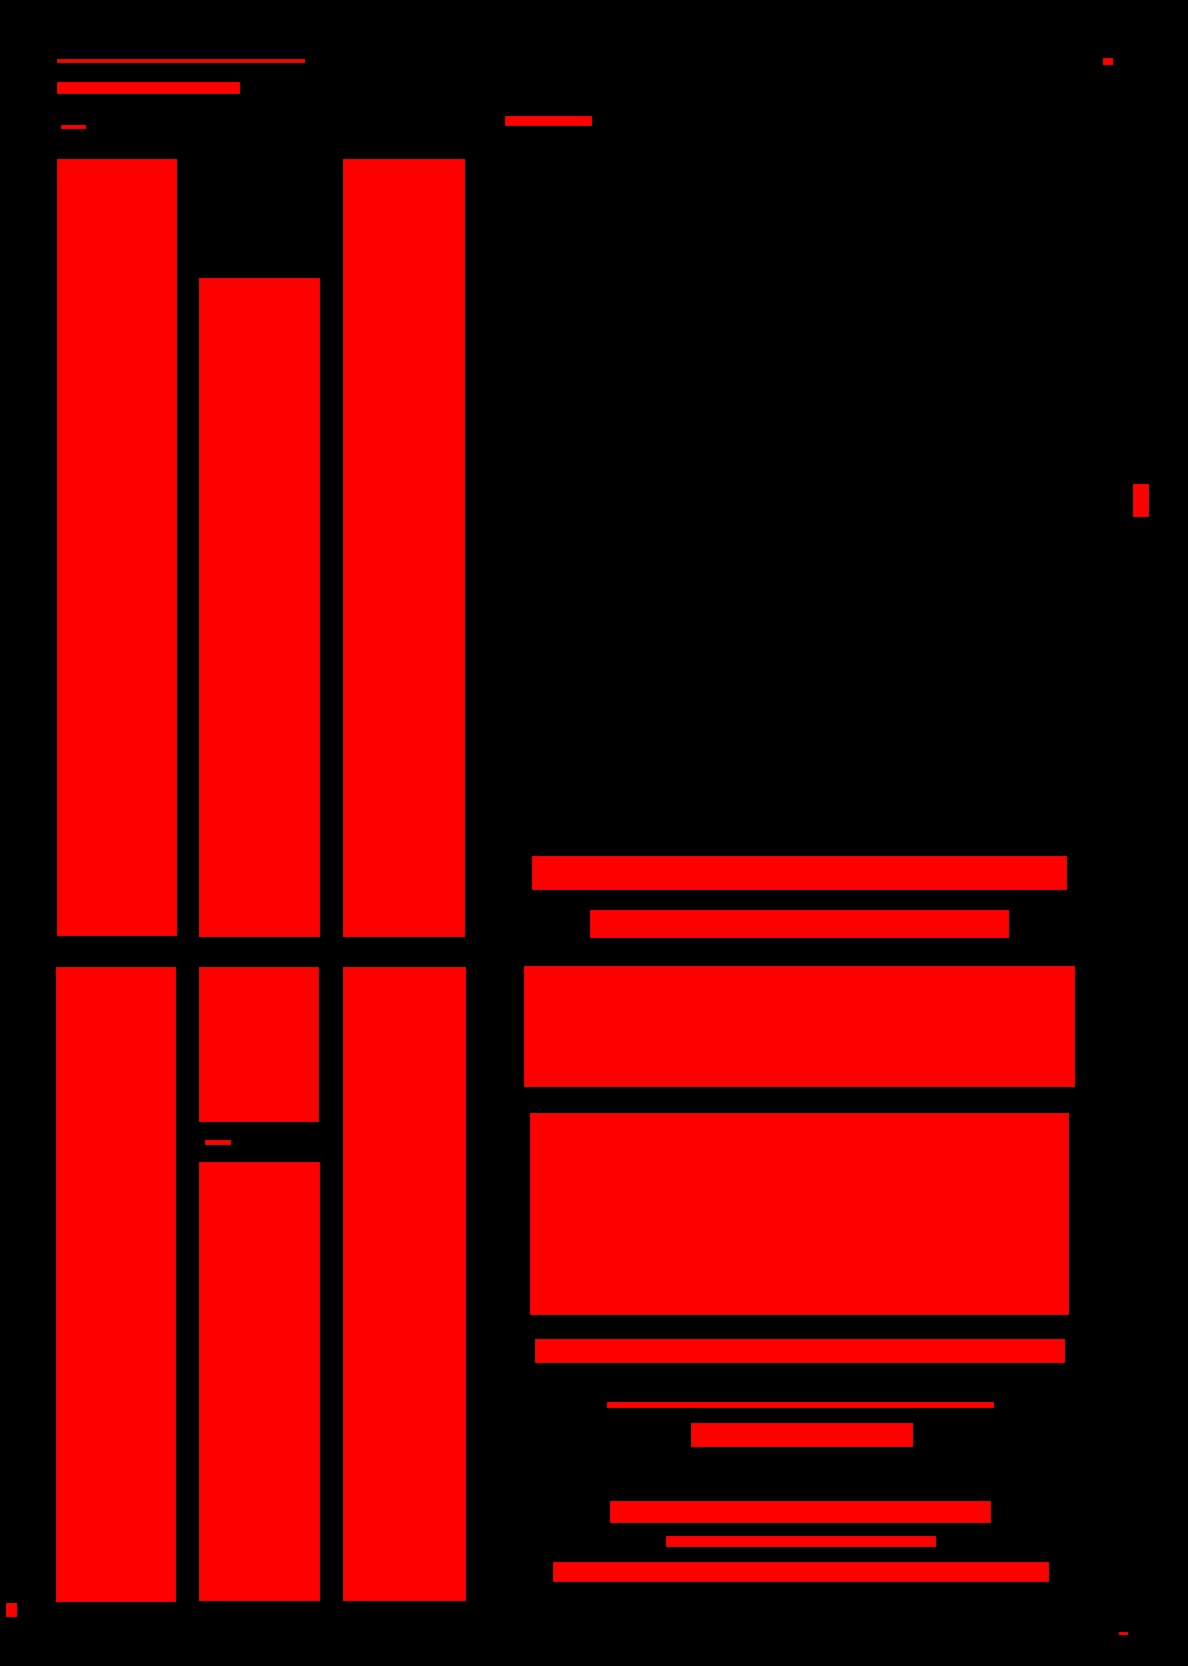
\includegraphics[width=0.99\linewidth, clip=true, trim = 0mm 0mm 0mm 0mm]{figures/ocr/9rwJ51v.jpg}
  \caption{OCR}
\end{subfigure}%
\begin{subfigure}{.25\textwidth}
  \centering
  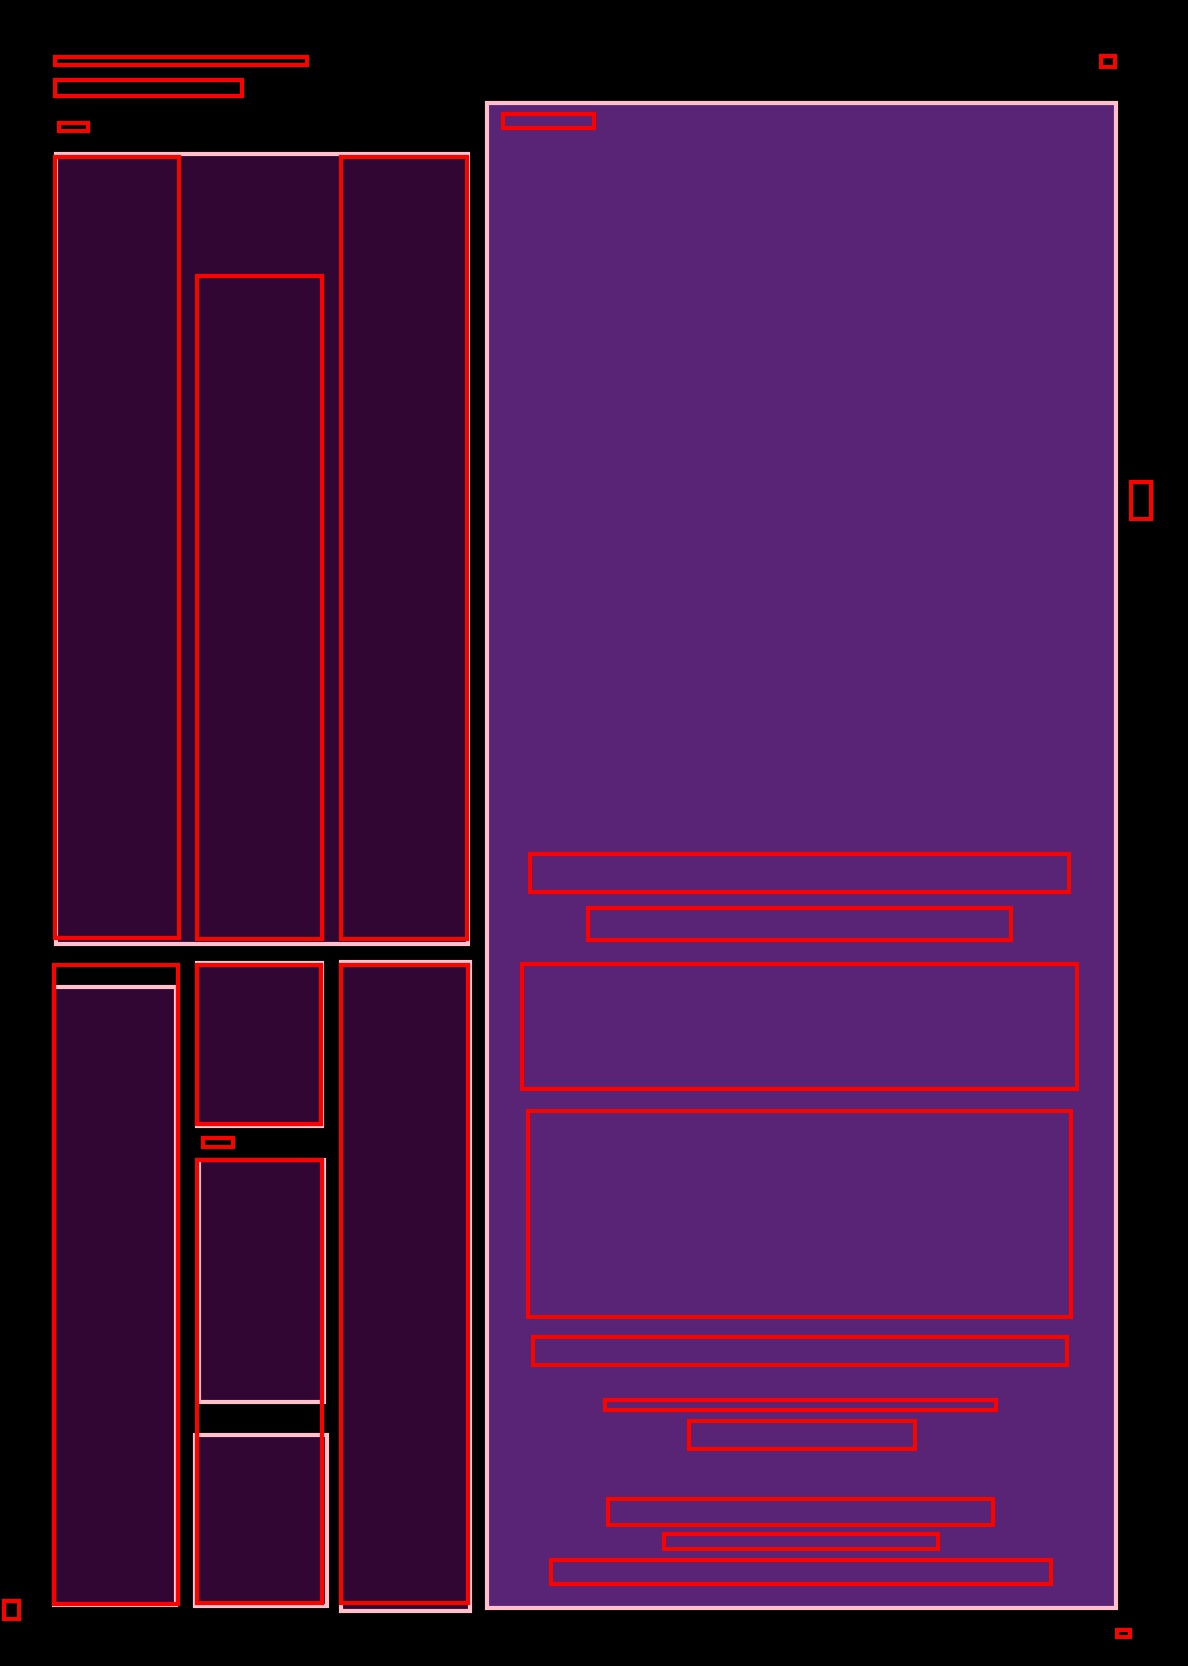
\includegraphics[width=0.99\linewidth, clip=true, trim = 0mm 0mm 0mm 0mm]{figures/ocr_bbox/9rwJ51v.jpg}
  \caption{GT Label + OCR}
\end{subfigure}%
\begin{subfigure}{.25\textwidth}
  \centering
  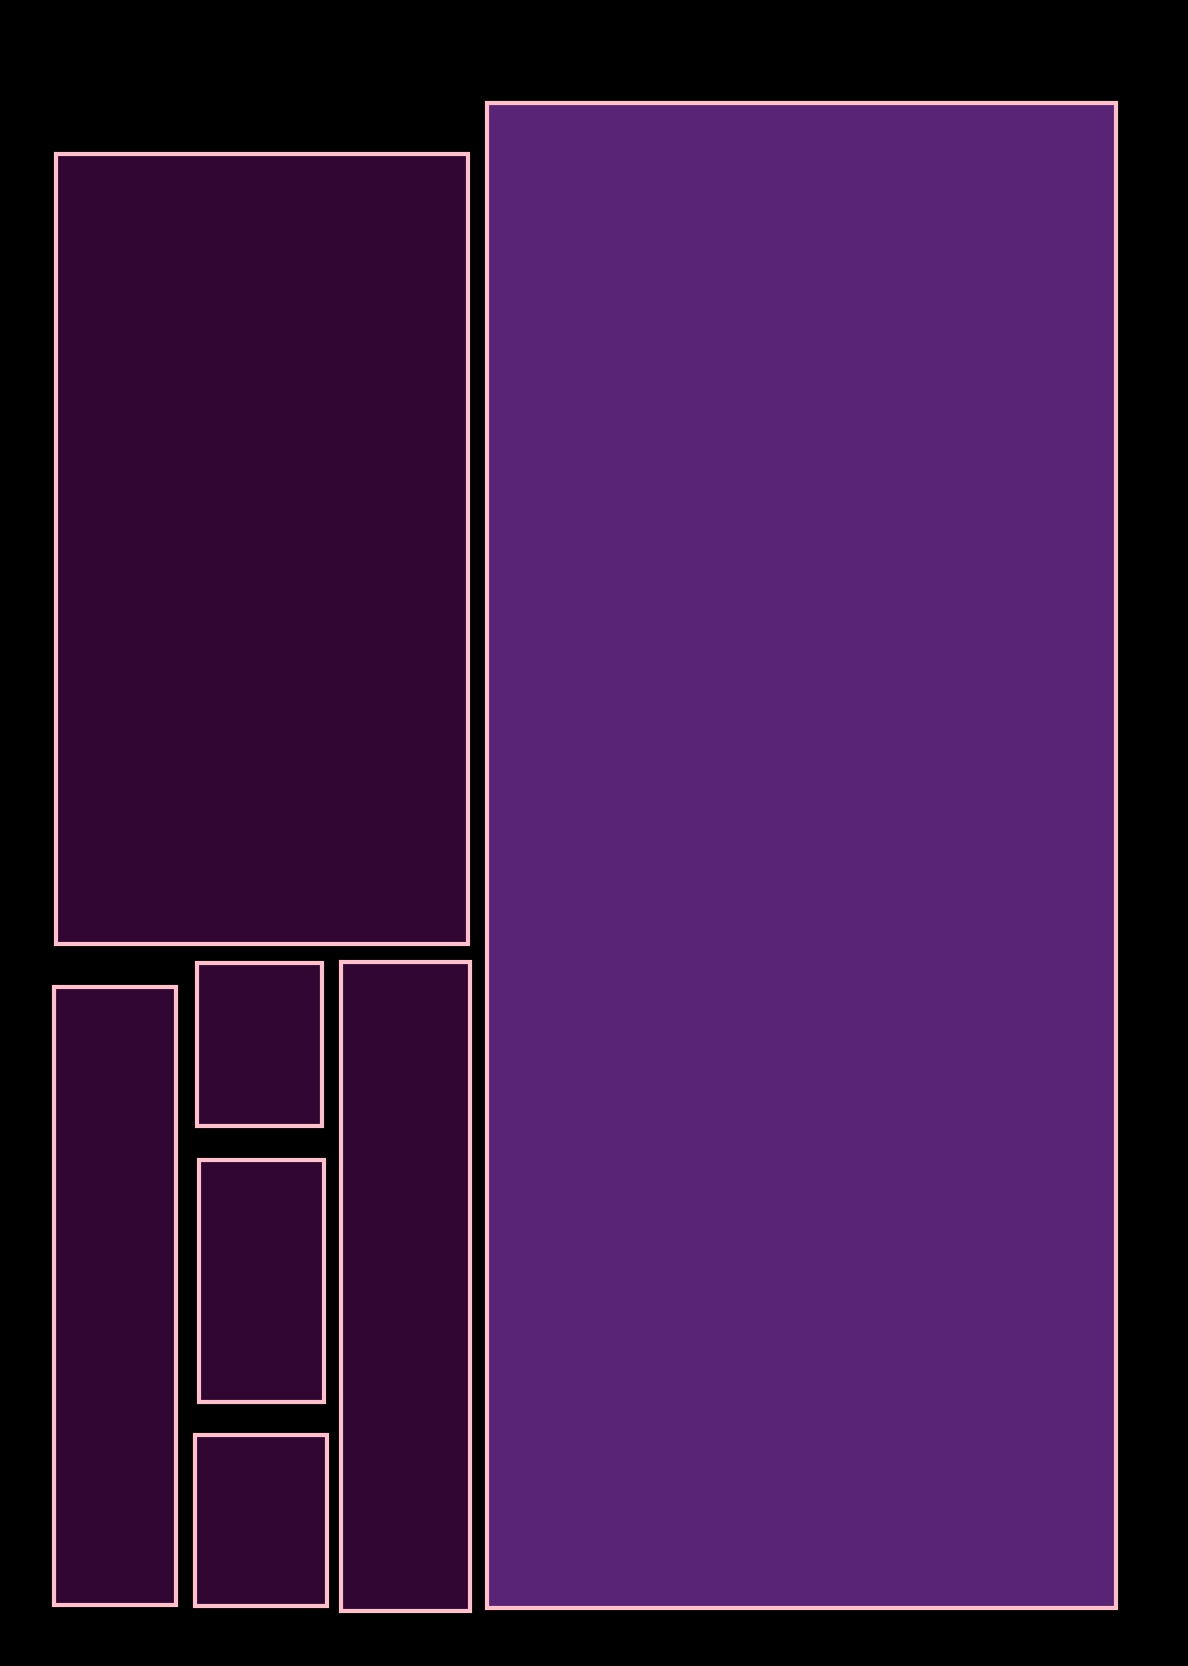
\includegraphics[width=0.99\linewidth, clip=true, trim = 0mm 0mm 0mm 0mm]{figures/bbox/9rwJ51v.jpg}
  \caption{GT Label}
\end{subfigure}%
\begin{subfigure}{.25\textwidth}
  \centering
  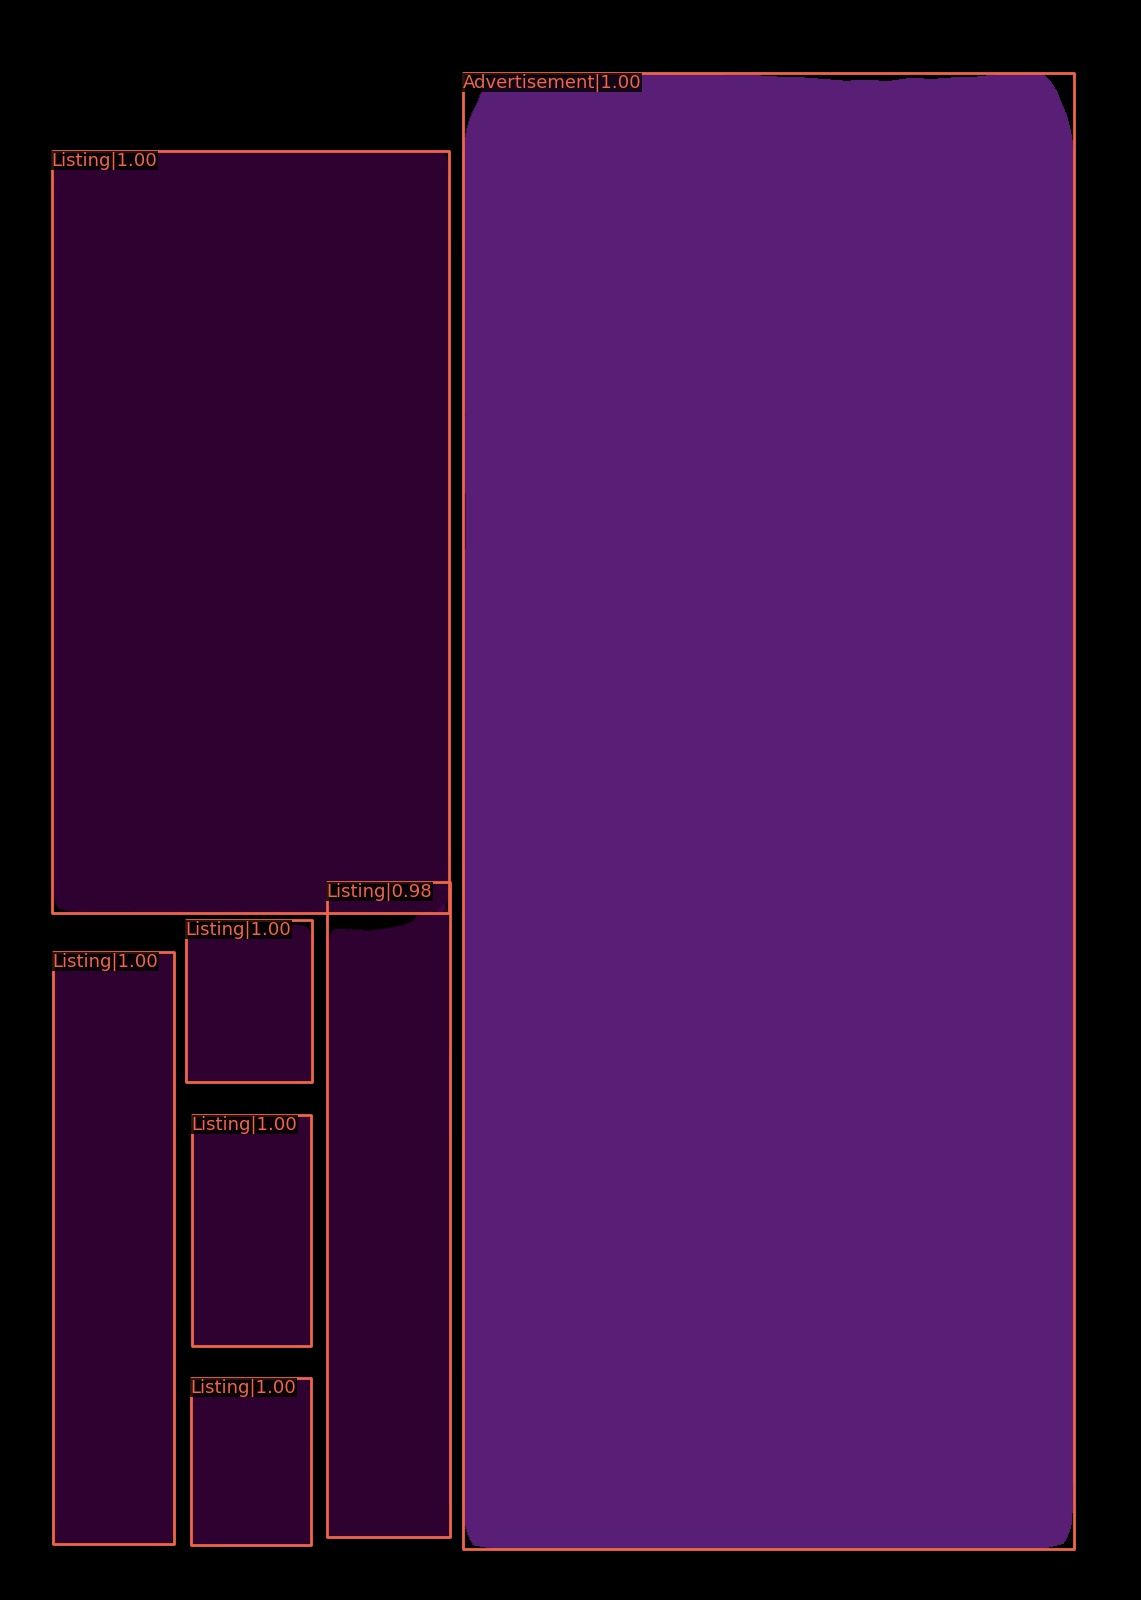
\includegraphics[width=0.99\linewidth, clip=true, trim = 0mm 0mm 0mm 0mm]{figures/labels-vanilla-0.75/9rwJ51v.jpg}
  \caption{Model prediction}
\end{subfigure}
\caption{A newspaper page with listings of TV/Radio timetables + advertisement.}
\label{fig:stocks}
\end{figure}
\end{frame}
\normalpage

%%%%%%%%%%%%%%%%%%%%%%%%%%%%%%%%%%%%%%%%%%%%%%%%%%%%%%%%%%%%
\begin{frame}
  \begin{figure}
\centering
\begin{subfigure}{.25\textwidth}
  \centering
  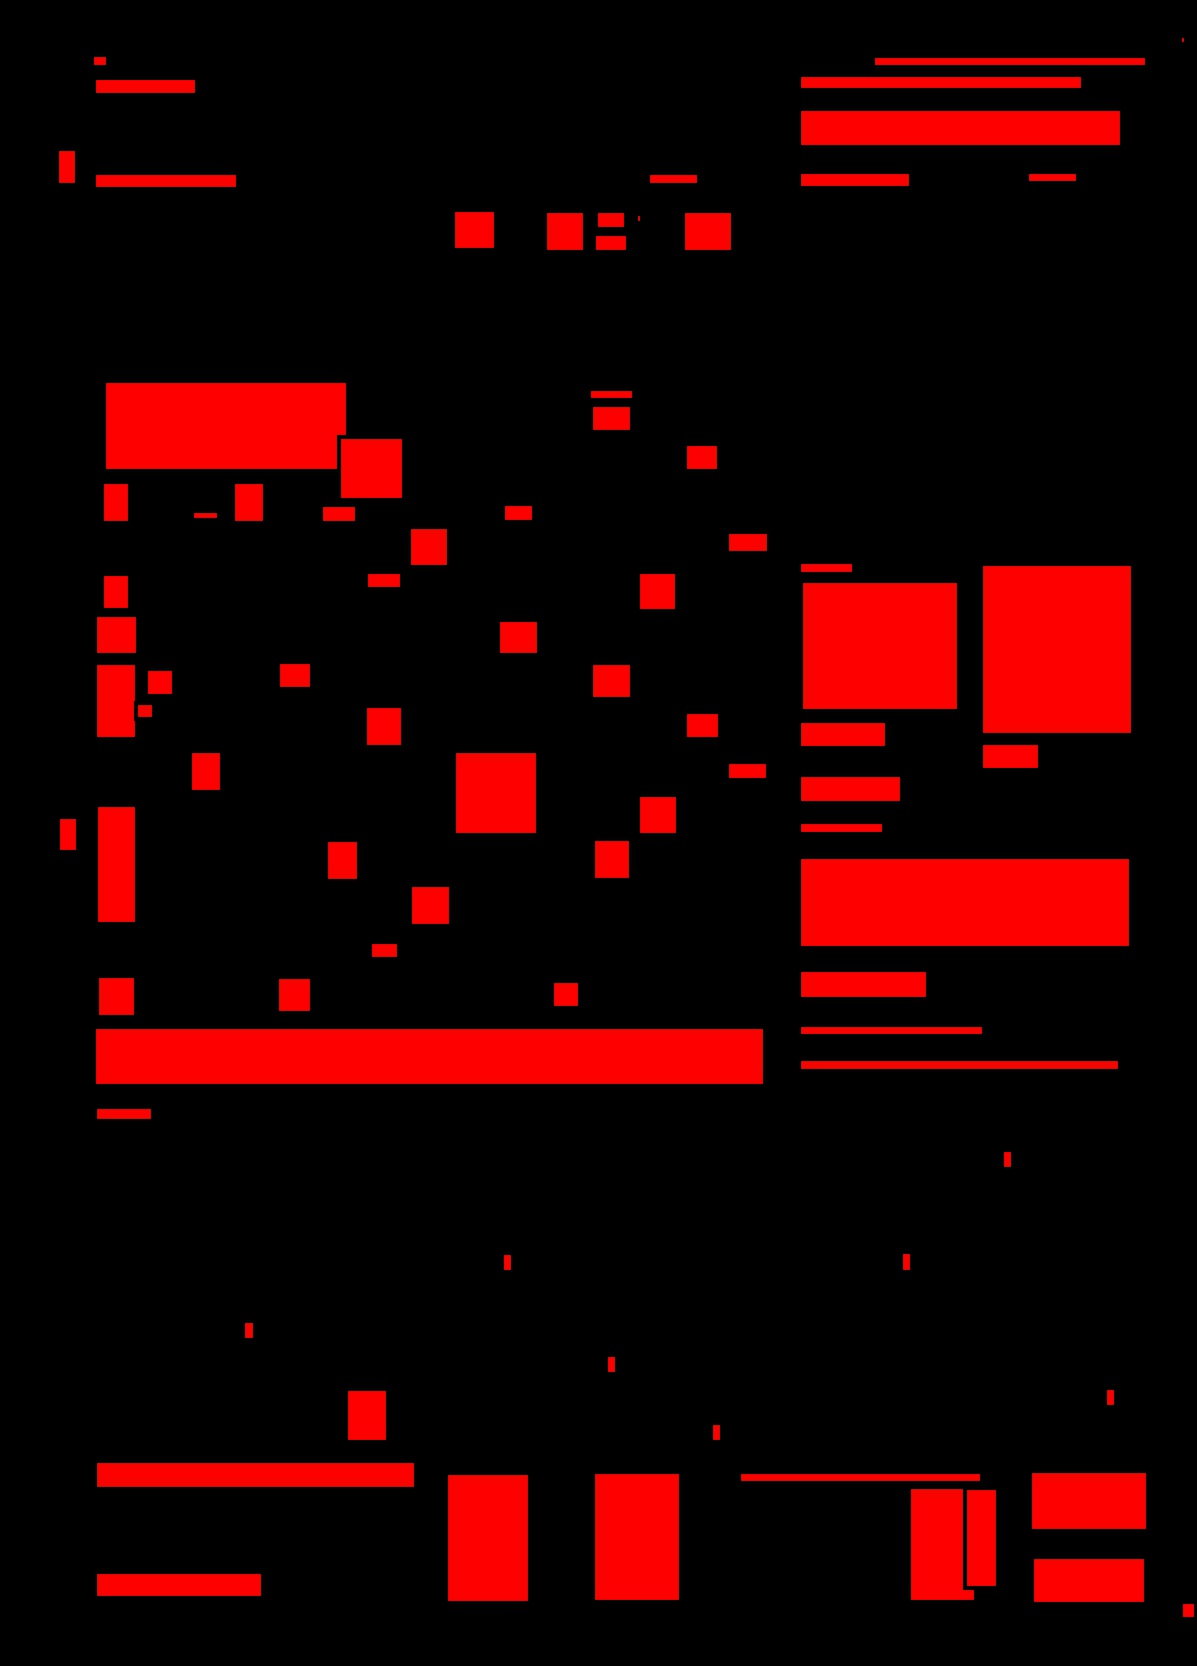
\includegraphics[width=0.99\linewidth, clip=true, trim = 0mm 0mm 0mm 0mm]{figures/ocr/y3LXnnL.jpg}
  \caption{OCR}
\end{subfigure}%
\begin{subfigure}{.25\textwidth}
  \centering
  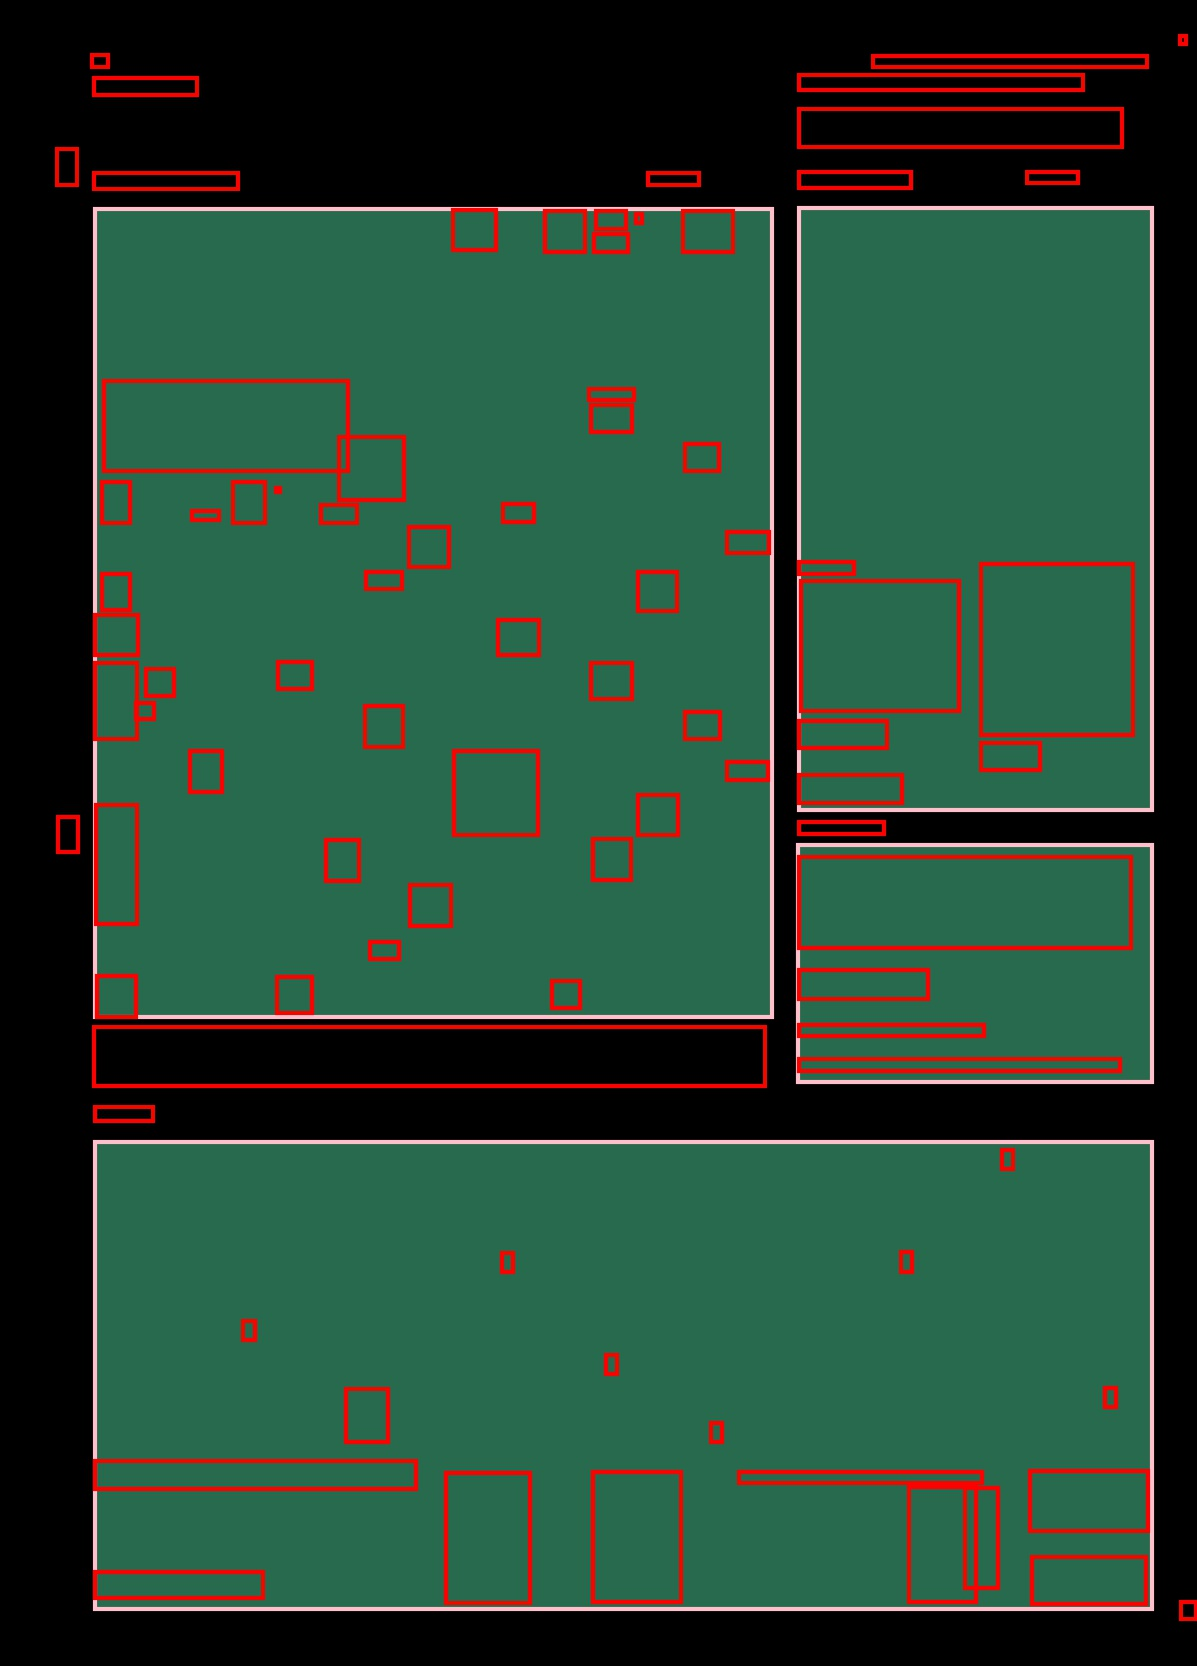
\includegraphics[width=0.99\linewidth, clip=true, trim = 0mm 0mm 0mm 0mm]{figures/ocr_bbox/y3LXnnL.jpg}
  \caption{GT Label + OCR}
\end{subfigure}%
\begin{subfigure}{.25\textwidth}
  \centering
  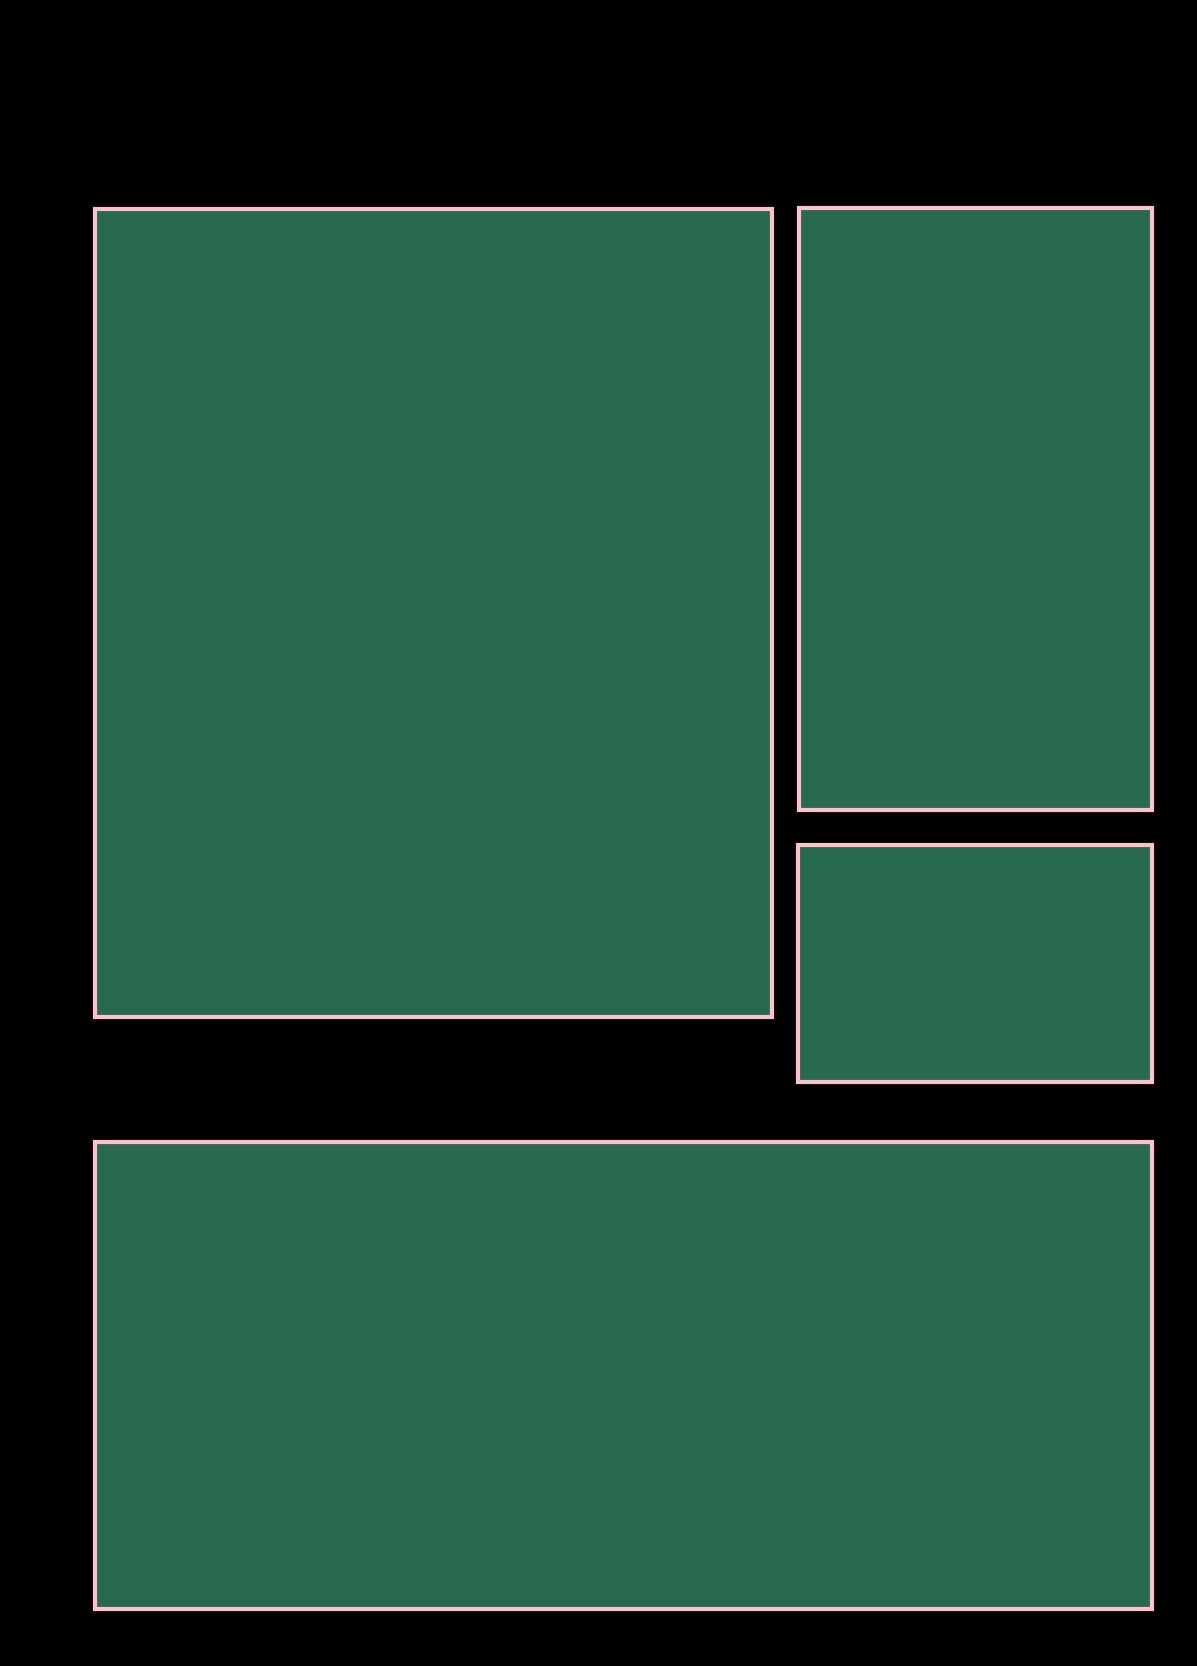
\includegraphics[width=0.99\linewidth, clip=true, trim = 0mm 0mm 0mm 0mm]{figures/bbox/y3LXnnL.jpg}
  \caption{GT Label}
\end{subfigure}%
\begin{subfigure}{.25\textwidth}
  \centering
  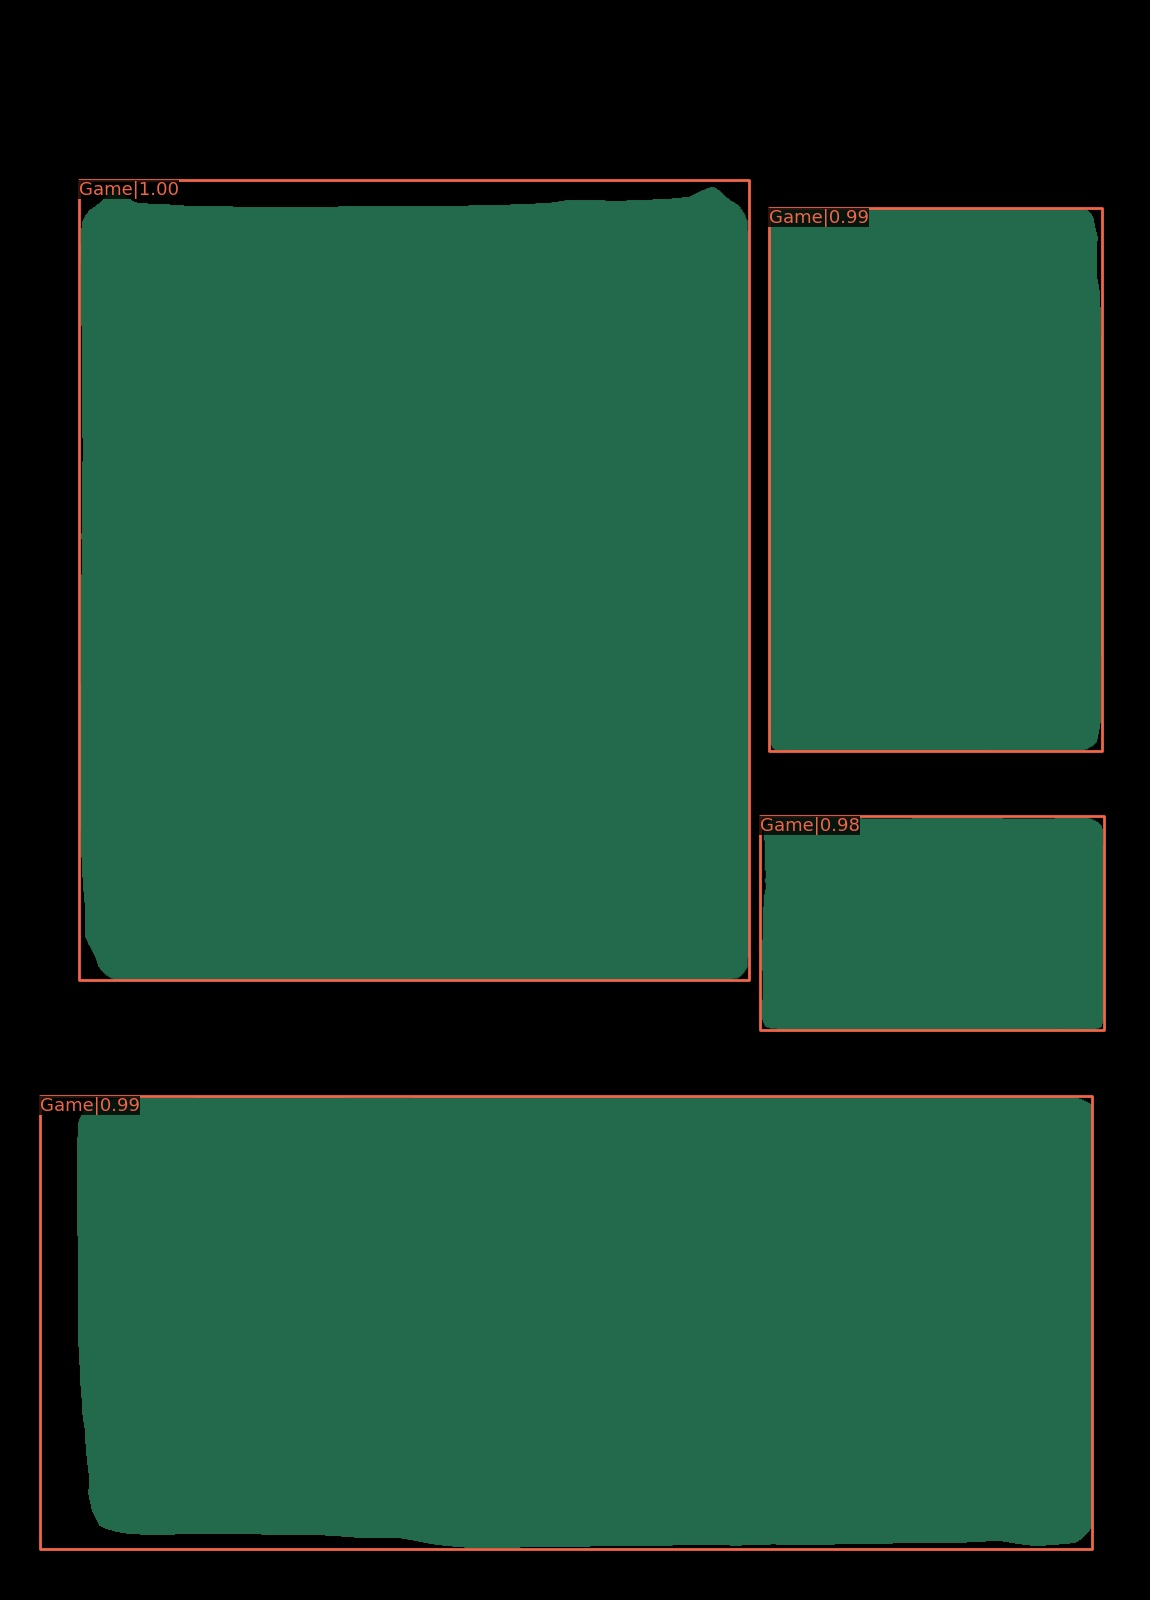
\includegraphics[width=0.99\linewidth, clip=true, trim = 0mm 0mm 0mm 0mm]{figures/labels-vanilla-0.75/y3LXnnL.jpg}
  \caption{Model prediction}
\end{subfigure}
\caption{A newspaper page with different types of games.}
\label{fig:stocks}
\end{figure}
\end{frame}
\normalpage

%%%%%%%%%%%%%%%%%%%%%%%%%%%%%%%%%%%%%%%%%%%%%%%%%%%%%%%%%%%%
\begin{frame}
  \begin{figure}
\centering
\begin{subfigure}{.25\textwidth}
  \centering
  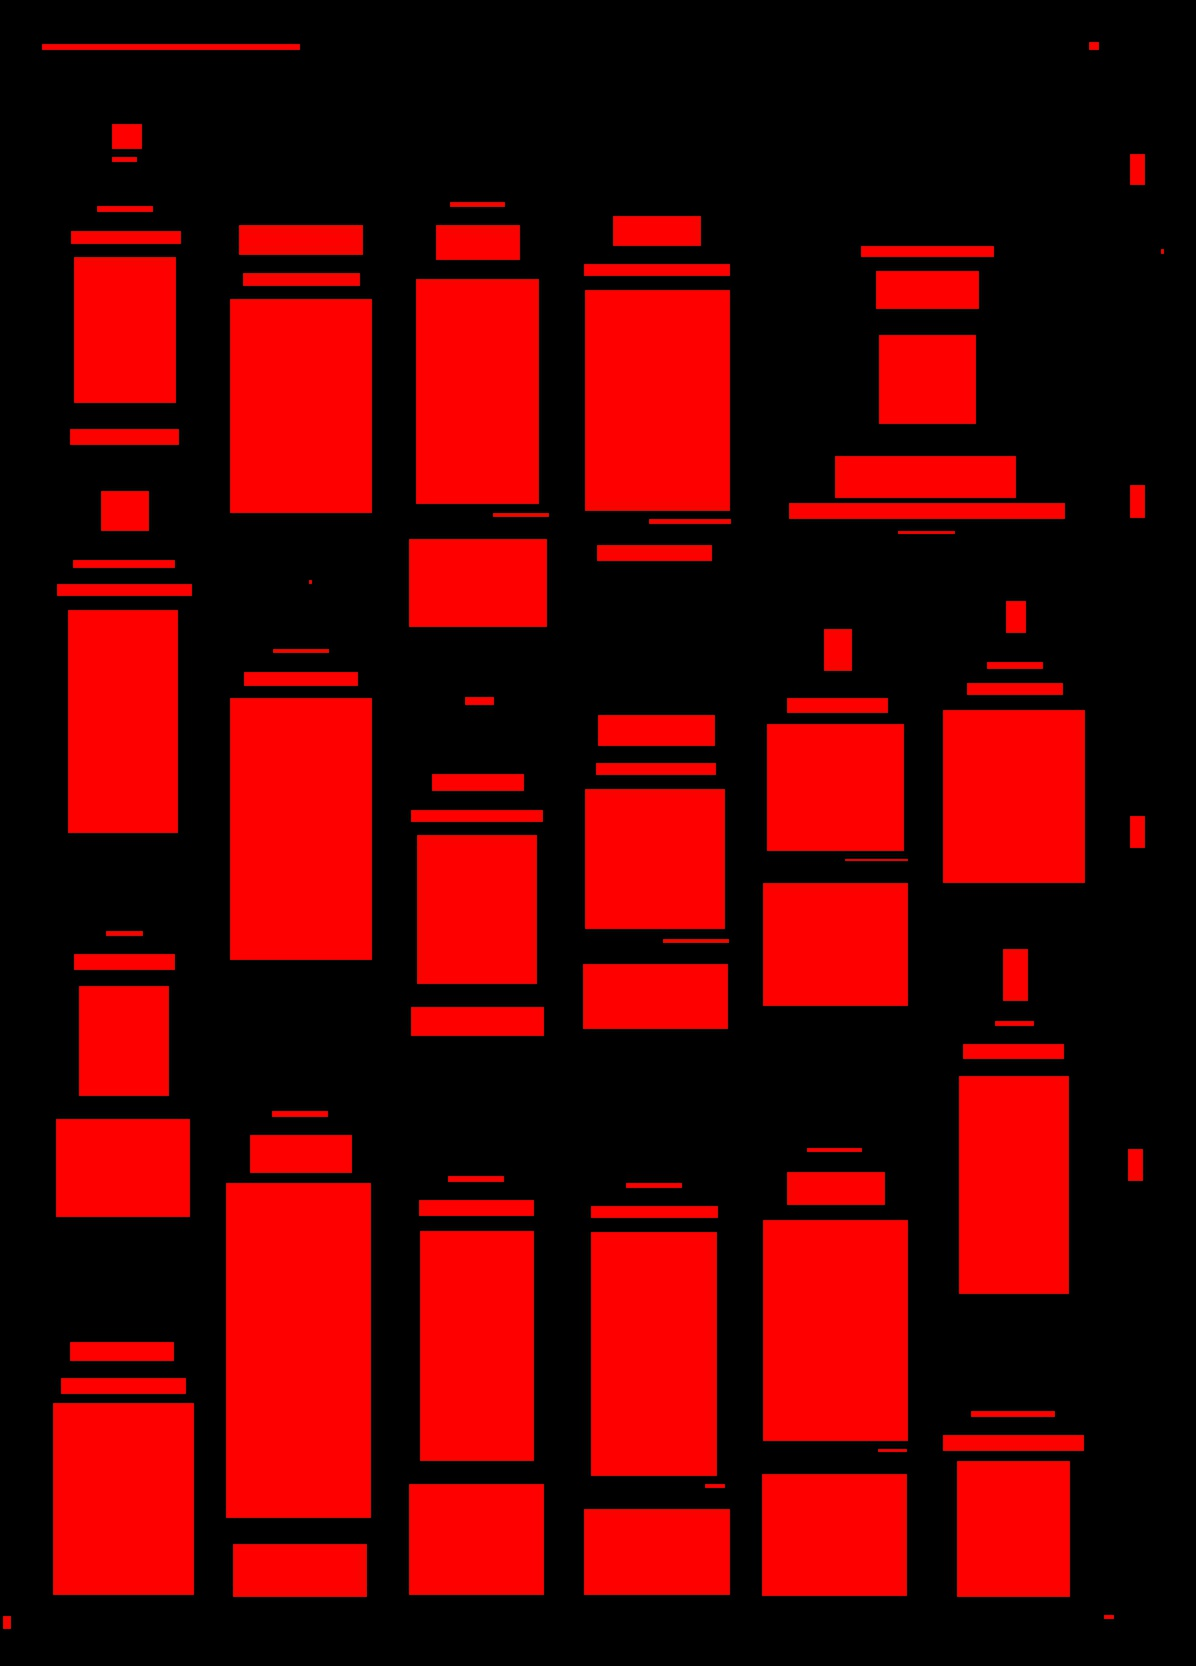
\includegraphics[width=0.99\linewidth, clip=true, trim = 0mm 0mm 0mm 0mm]{figures/ocr/GQU6vjW.jpg}
  \caption{OCR}
\end{subfigure}%
\begin{subfigure}{.25\textwidth}
  \centering
  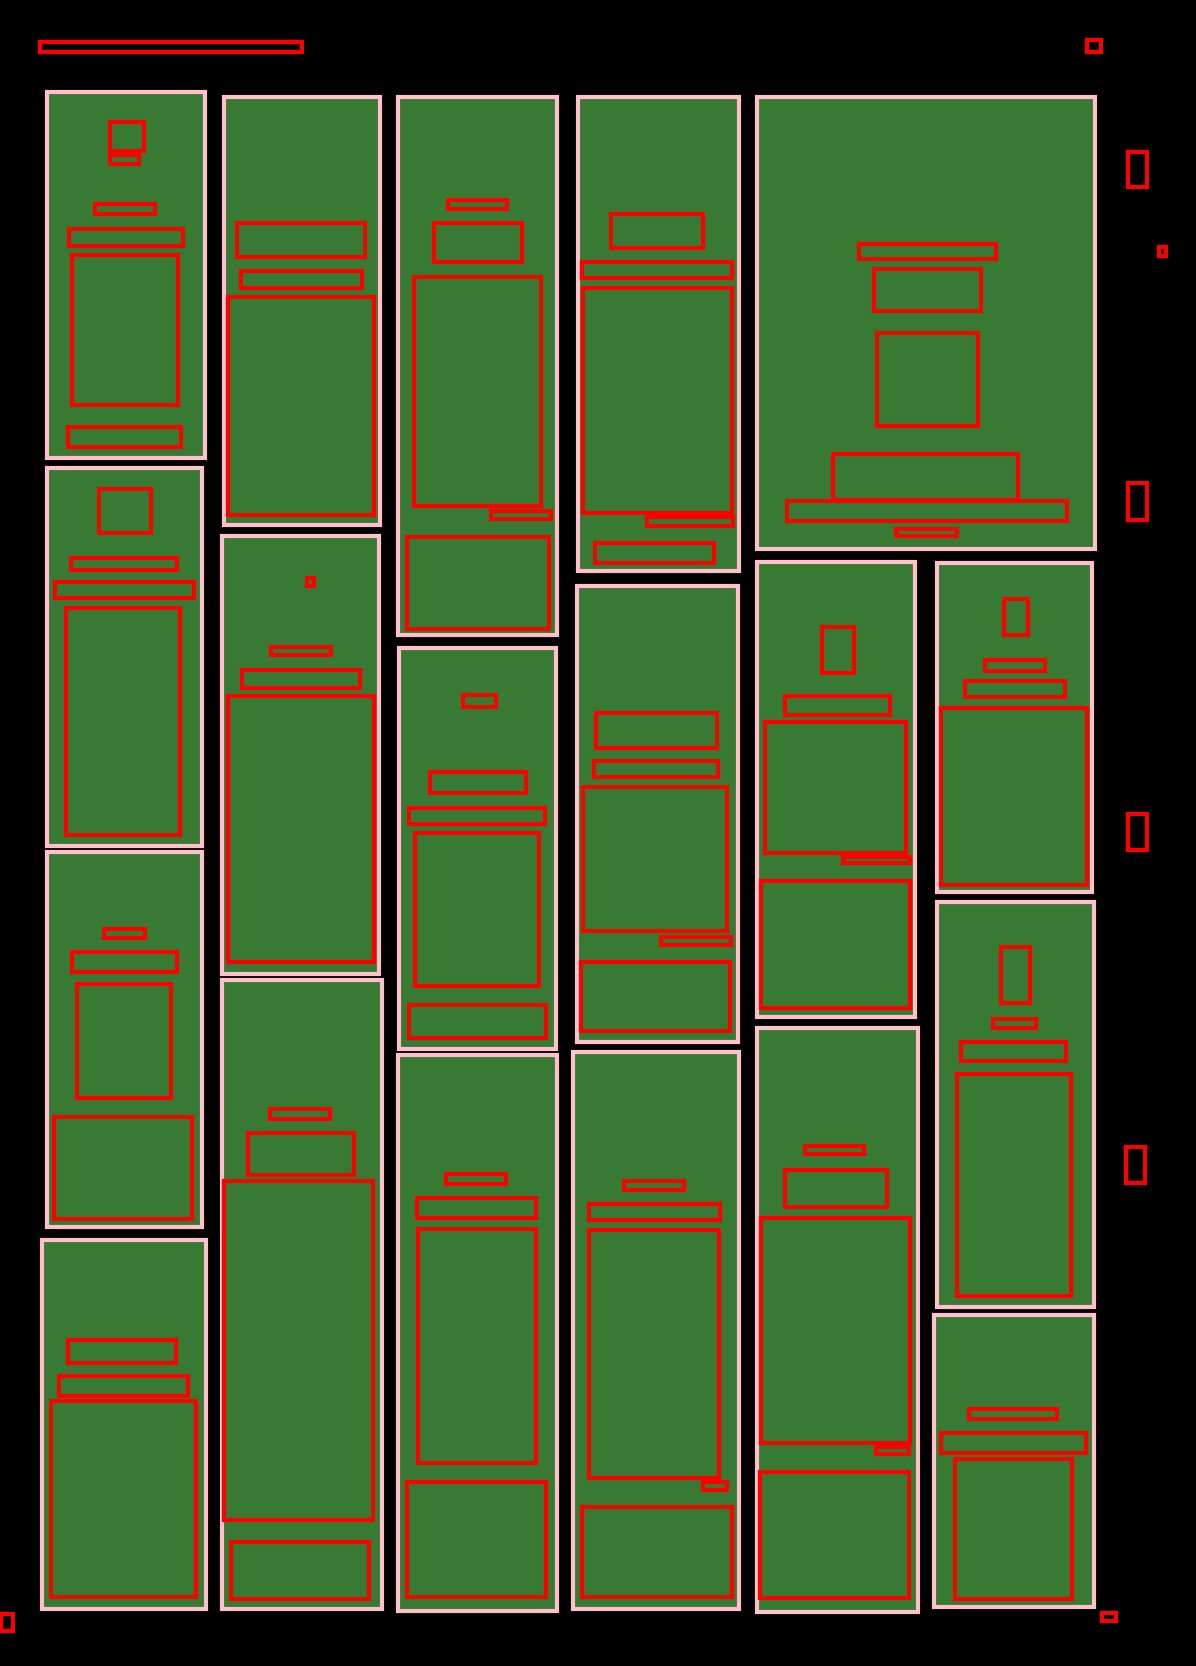
\includegraphics[width=0.99\linewidth, clip=true, trim = 0mm 0mm 0mm 0mm]{figures/ocr_bbox/GQU6vjW.jpg}
  \caption{GT Label + OCR}
\end{subfigure}%
\begin{subfigure}{.25\textwidth}
  \centering
  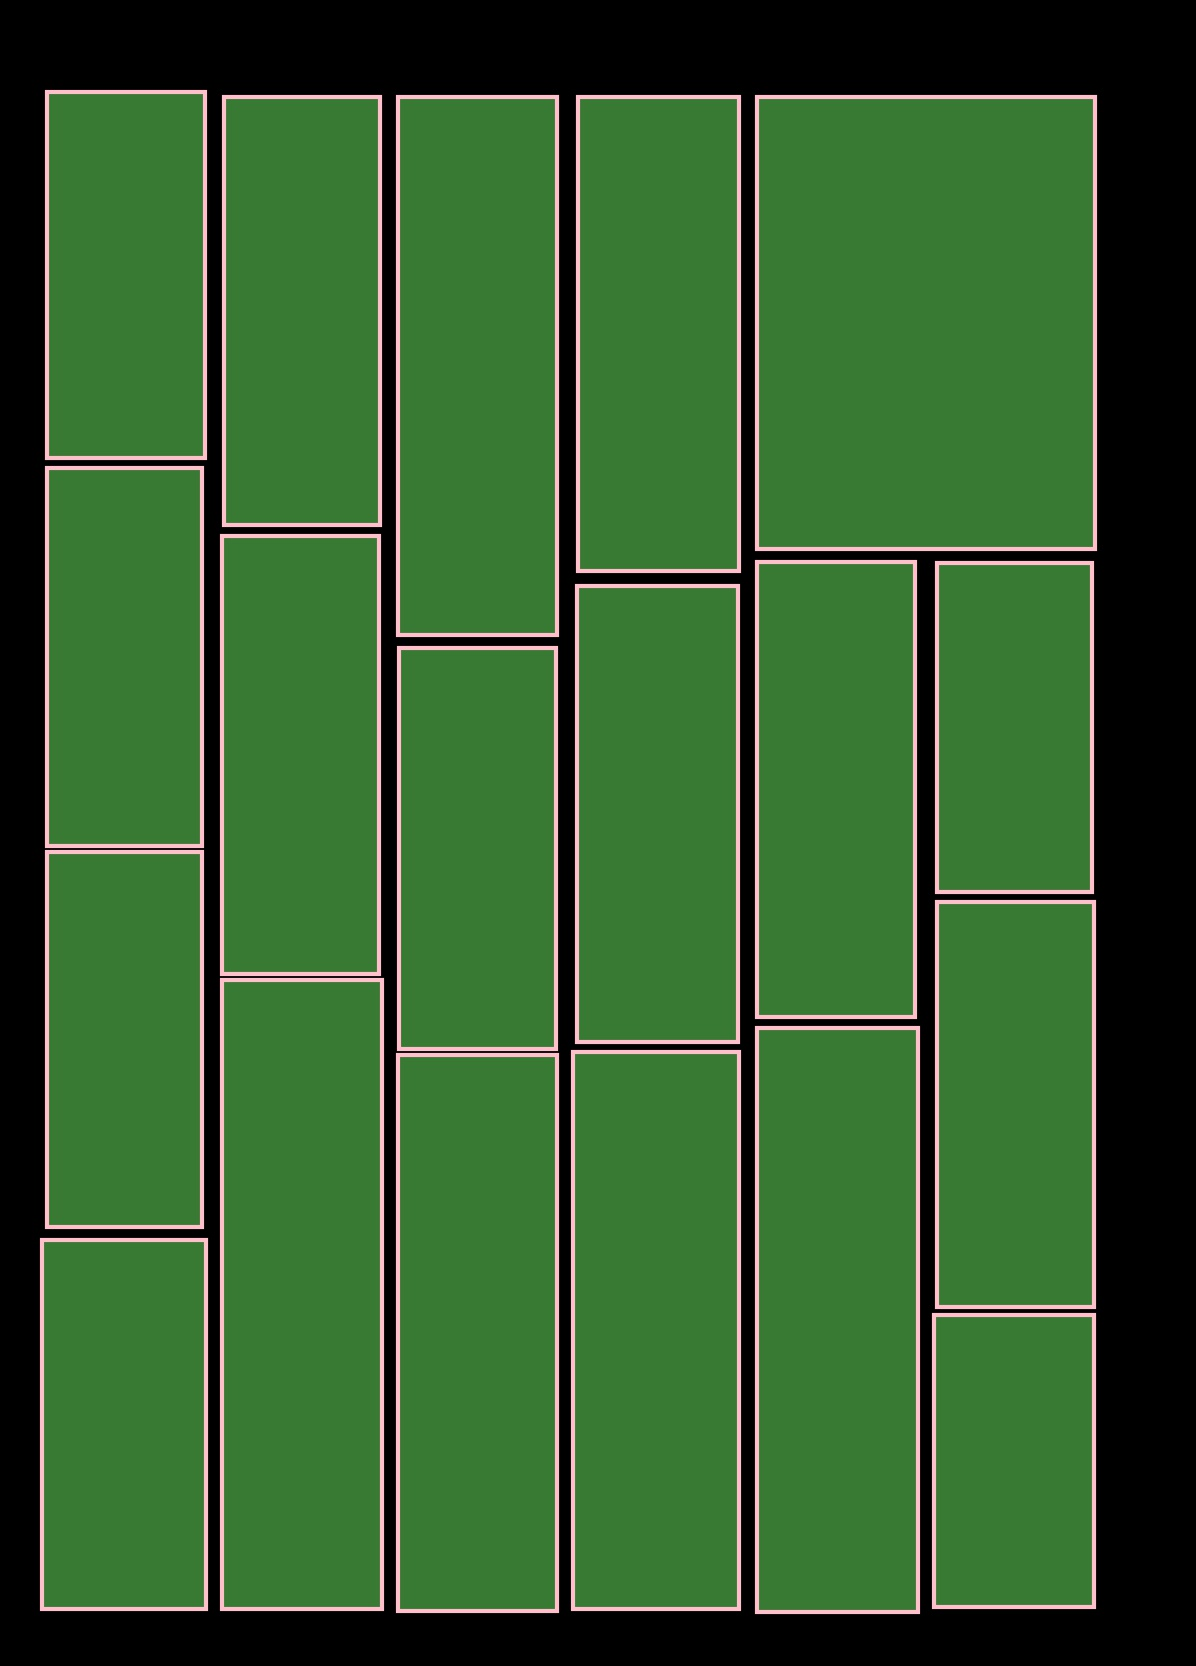
\includegraphics[width=0.99\linewidth, clip=true, trim = 0mm 0mm 0mm 0mm]{figures/bbox/GQU6vjW.jpg}
  \caption{GT Label}
\end{subfigure}%
\begin{subfigure}{.25\textwidth}
  \centering
  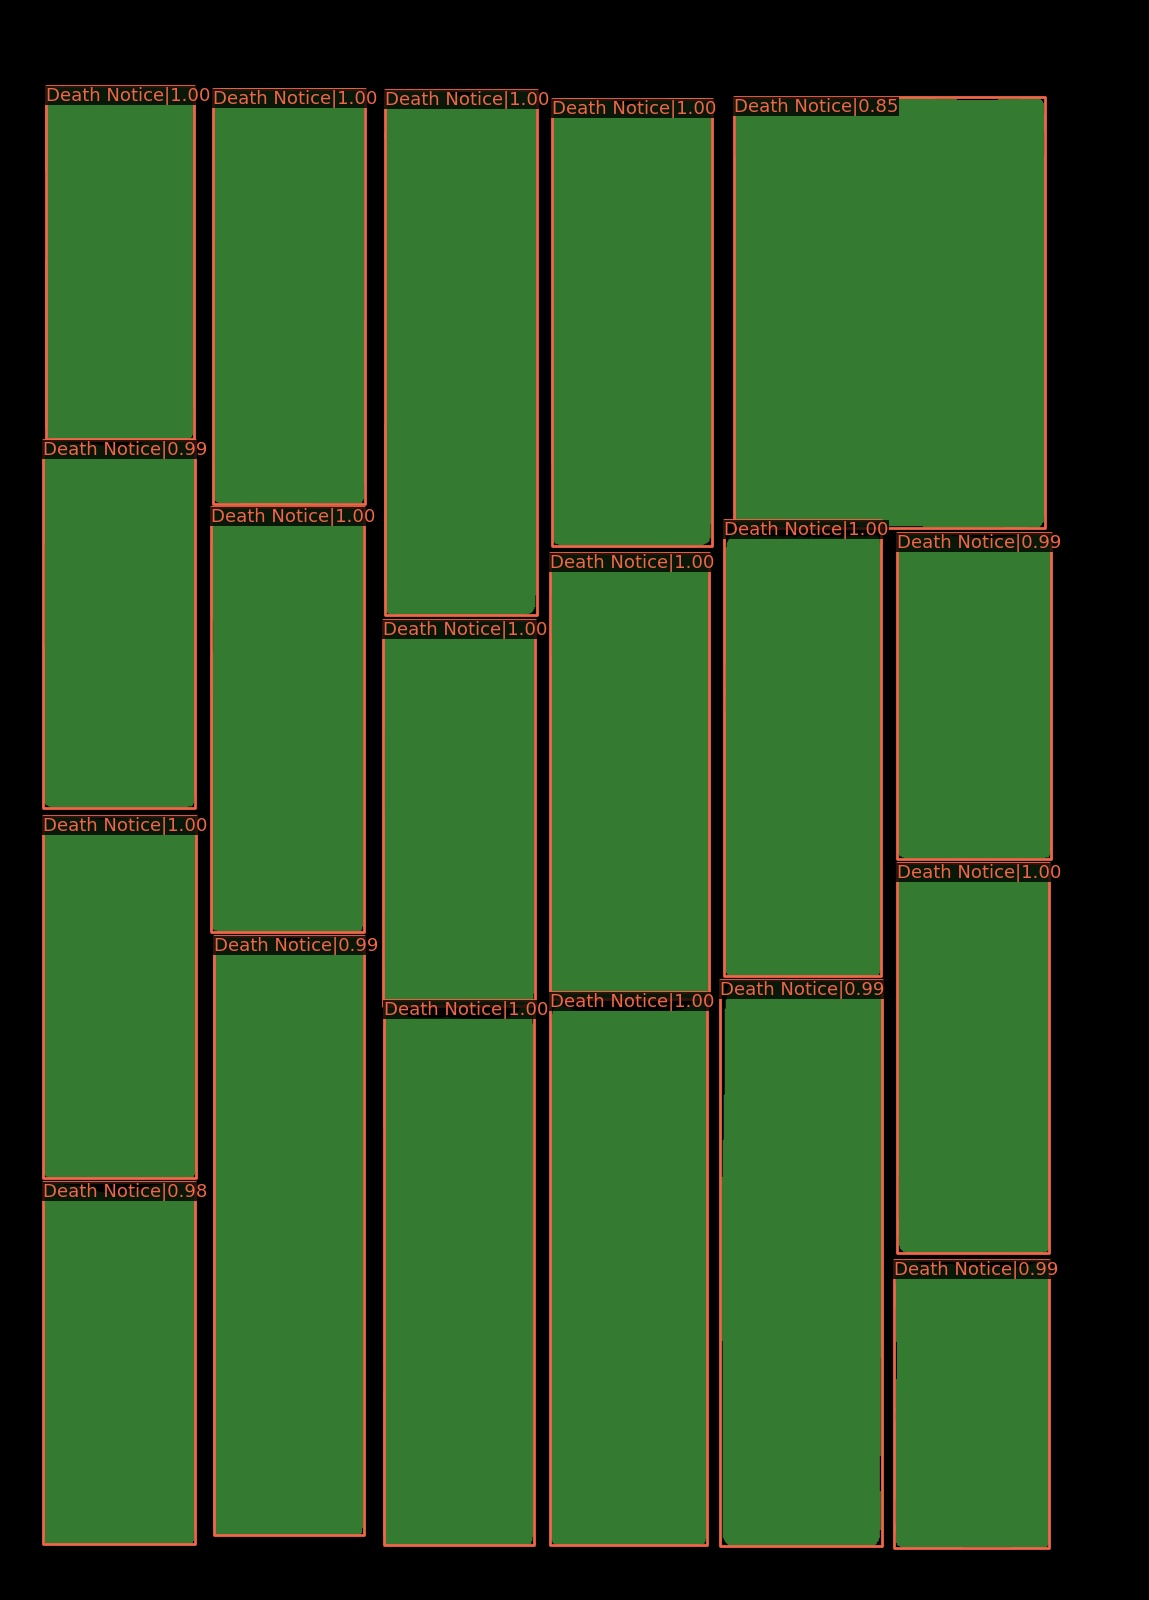
\includegraphics[width=0.99\linewidth, clip=true, trim = 0mm 0mm 0mm 0mm]{figures/labels-vanilla-0.75/GQU6vjW.jpg}
  \caption{Model prediction}
\end{subfigure}
\caption{A newspaper page with obituaries.}
\label{fig:obituaries}
\end{figure}
\end{frame}
\normalpage

%%%%%%%%%%%%%%%%%%%%%%%%%%%%%%%%%%%%%%%%%%%%%%%%%%%%%%%%%%%%
\begin{frame}
  \begin{figure}
\centering
\begin{subfigure}{.25\textwidth}
  \centering
  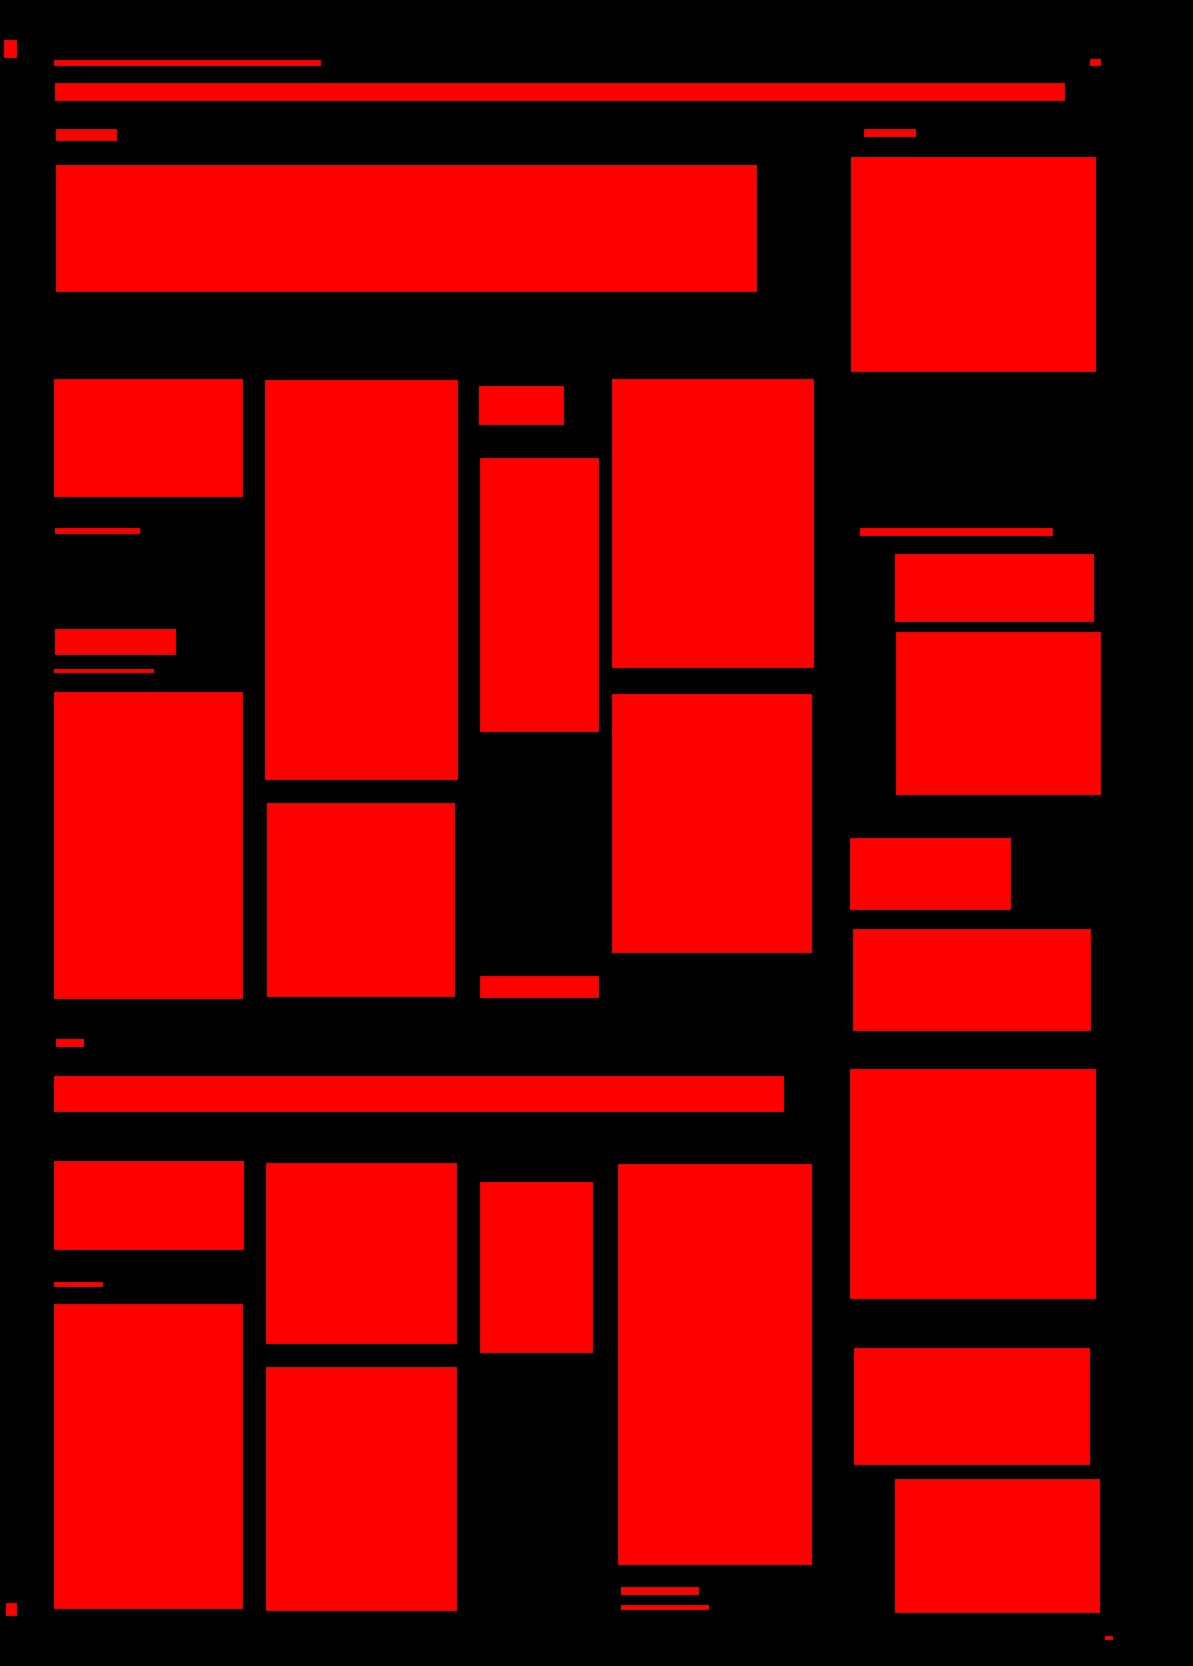
\includegraphics[width=0.99\linewidth, clip=true, trim = 0mm 0mm 0mm 0mm]{figures/ocr/AVThDFz.jpg}
  \caption{OCR}
\end{subfigure}%
\begin{subfigure}{.25\textwidth}
  \centering
  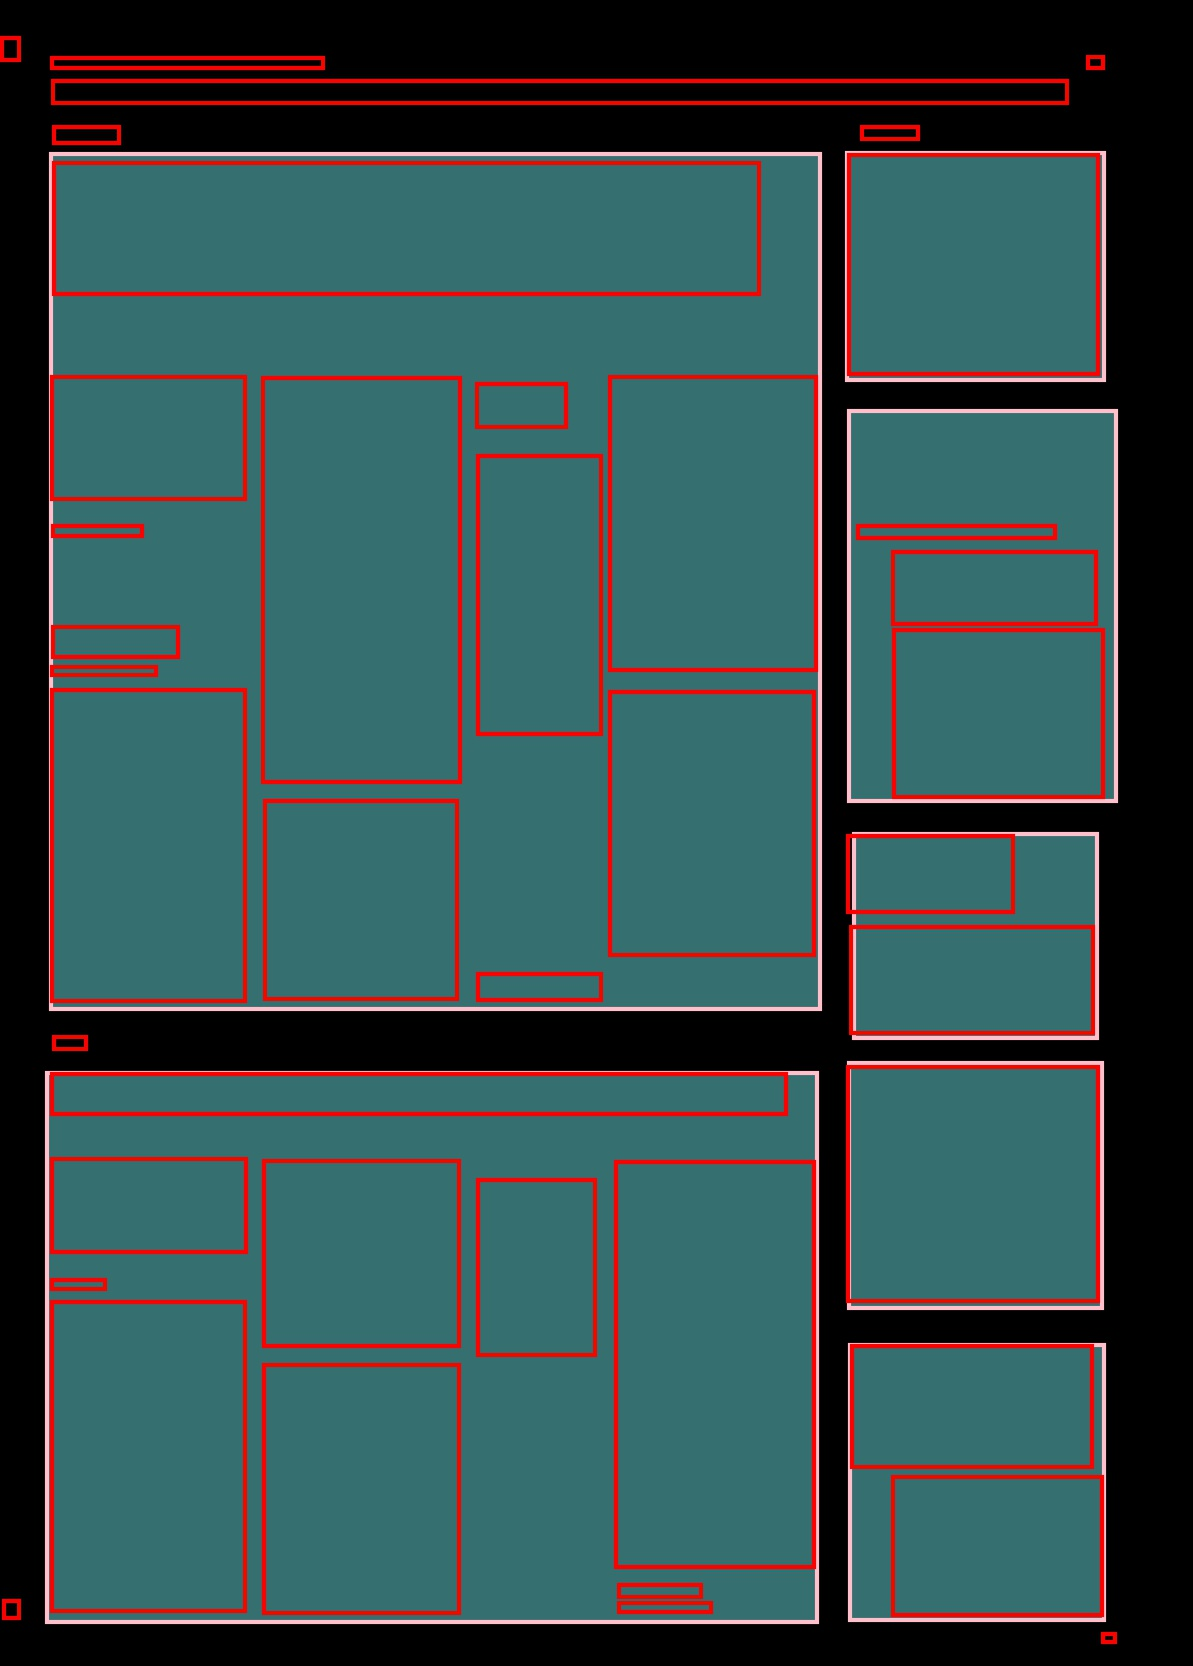
\includegraphics[width=0.99\linewidth, clip=true, trim = 0mm 0mm 0mm 0mm]{figures/ocr_bbox/AVThDFz.jpg}
  \caption{GT Label + OCR}
\end{subfigure}%
\begin{subfigure}{.25\textwidth}
  \centering
  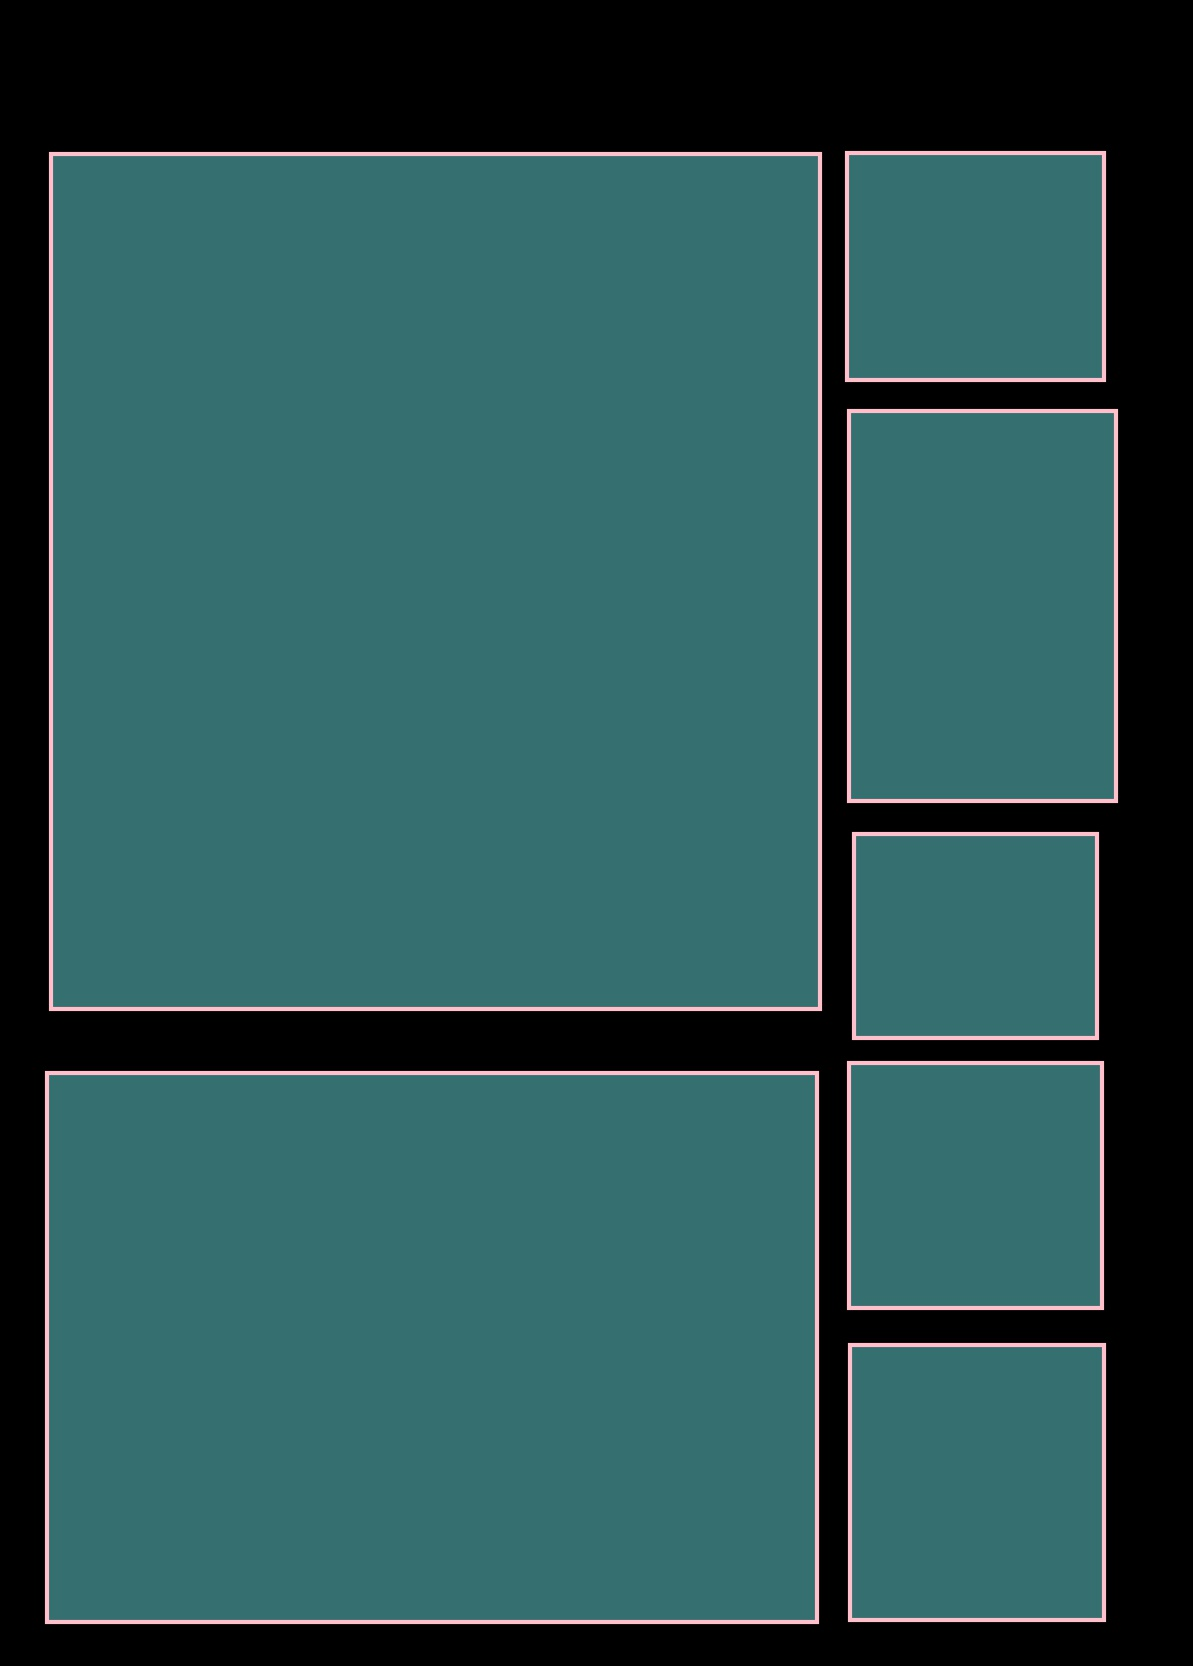
\includegraphics[width=0.99\linewidth, clip=true, trim = 0mm 0mm 0mm 0mm]{figures/bbox/AVThDFz.jpg}
  \caption{GT Label}
\end{subfigure}%
\begin{subfigure}{.25\textwidth}
  \centering
  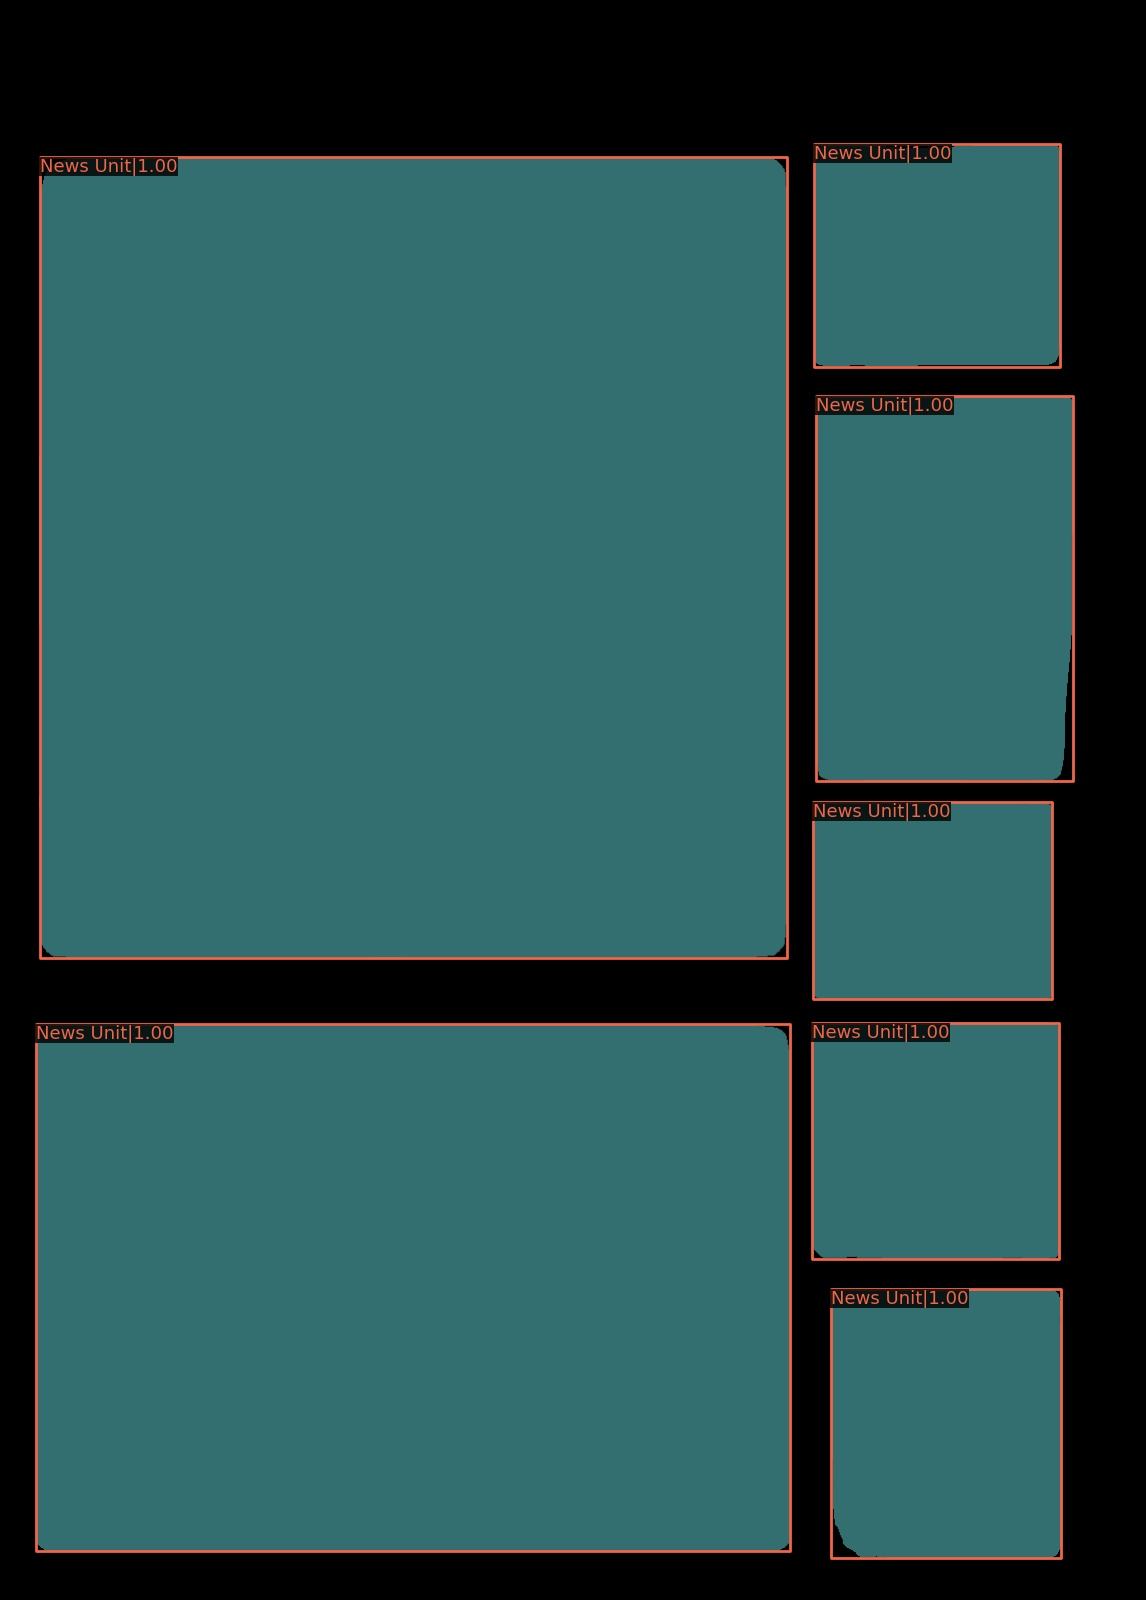
\includegraphics[width=0.99\linewidth, clip=true, trim = 0mm 0mm 0mm 0mm]{figures/labels-vanilla-0.75/AVThDFz.jpg}
  \caption{Model prediction}
\end{subfigure}
\caption{A newspaper page consisting of news articles.}
\label{fig:newsarticles}
\end{figure}
\end{frame}
\normalpage

%%%%%%%%%%%%%%%%%%%%%%%%%%%%%%%%%%%%%%%%%%%%%%%%%%%%%%%%%%%%
\begin{frame}
  \begin{figure}
\centering
\begin{subfigure}{.25\textwidth}
  \centering
  
\includegraphics[width=0.99\linewidth, clip=true, trim = 0mm 0mm 0mm 0mm]{figures/ocr/1RoKim0.jpg}
  \caption{OCR}
\end{subfigure}%
\begin{subfigure}{.25\textwidth}
  \centering
  
\includegraphics[width=0.99\linewidth, clip=true, trim = 0mm 0mm 0mm 0mm]{figures/ocr_bbox/1RoKim0.jpg}
  \caption{GT Label + OCR}
\end{subfigure}%
\begin{subfigure}{.25\textwidth}
  \centering
  
\includegraphics[width=0.99\linewidth, clip=true, trim = 0mm 0mm 0mm 0mm]{figures/bbox/1RoKim0.jpg}
  \caption{GT Label}
\end{subfigure}%
\begin{subfigure}{.25\textwidth}
  \centering
  
\includegraphics[width=0.99\linewidth, clip=true, trim = 0mm 0mm 0mm 0mm]{figures/labels-vanilla-0.75/1RoKim0.jpg}
  \caption{Model prediction}
\end{subfigure}
\caption{A newspaper page consisting of a single large image, part of a multi-page article}
\label{fig:weather}
\end{figure}
\end{frame}
\normalpage

%%%%%%%%%%%%%%%%%%%%%%%%%%%%%%%%%%%%%%%%%%%%%%%%%%%%%%%%%%%%
\begin{frame}
  \begin{figure}
\centering
\begin{subfigure}{.25\textwidth}
  \centering
  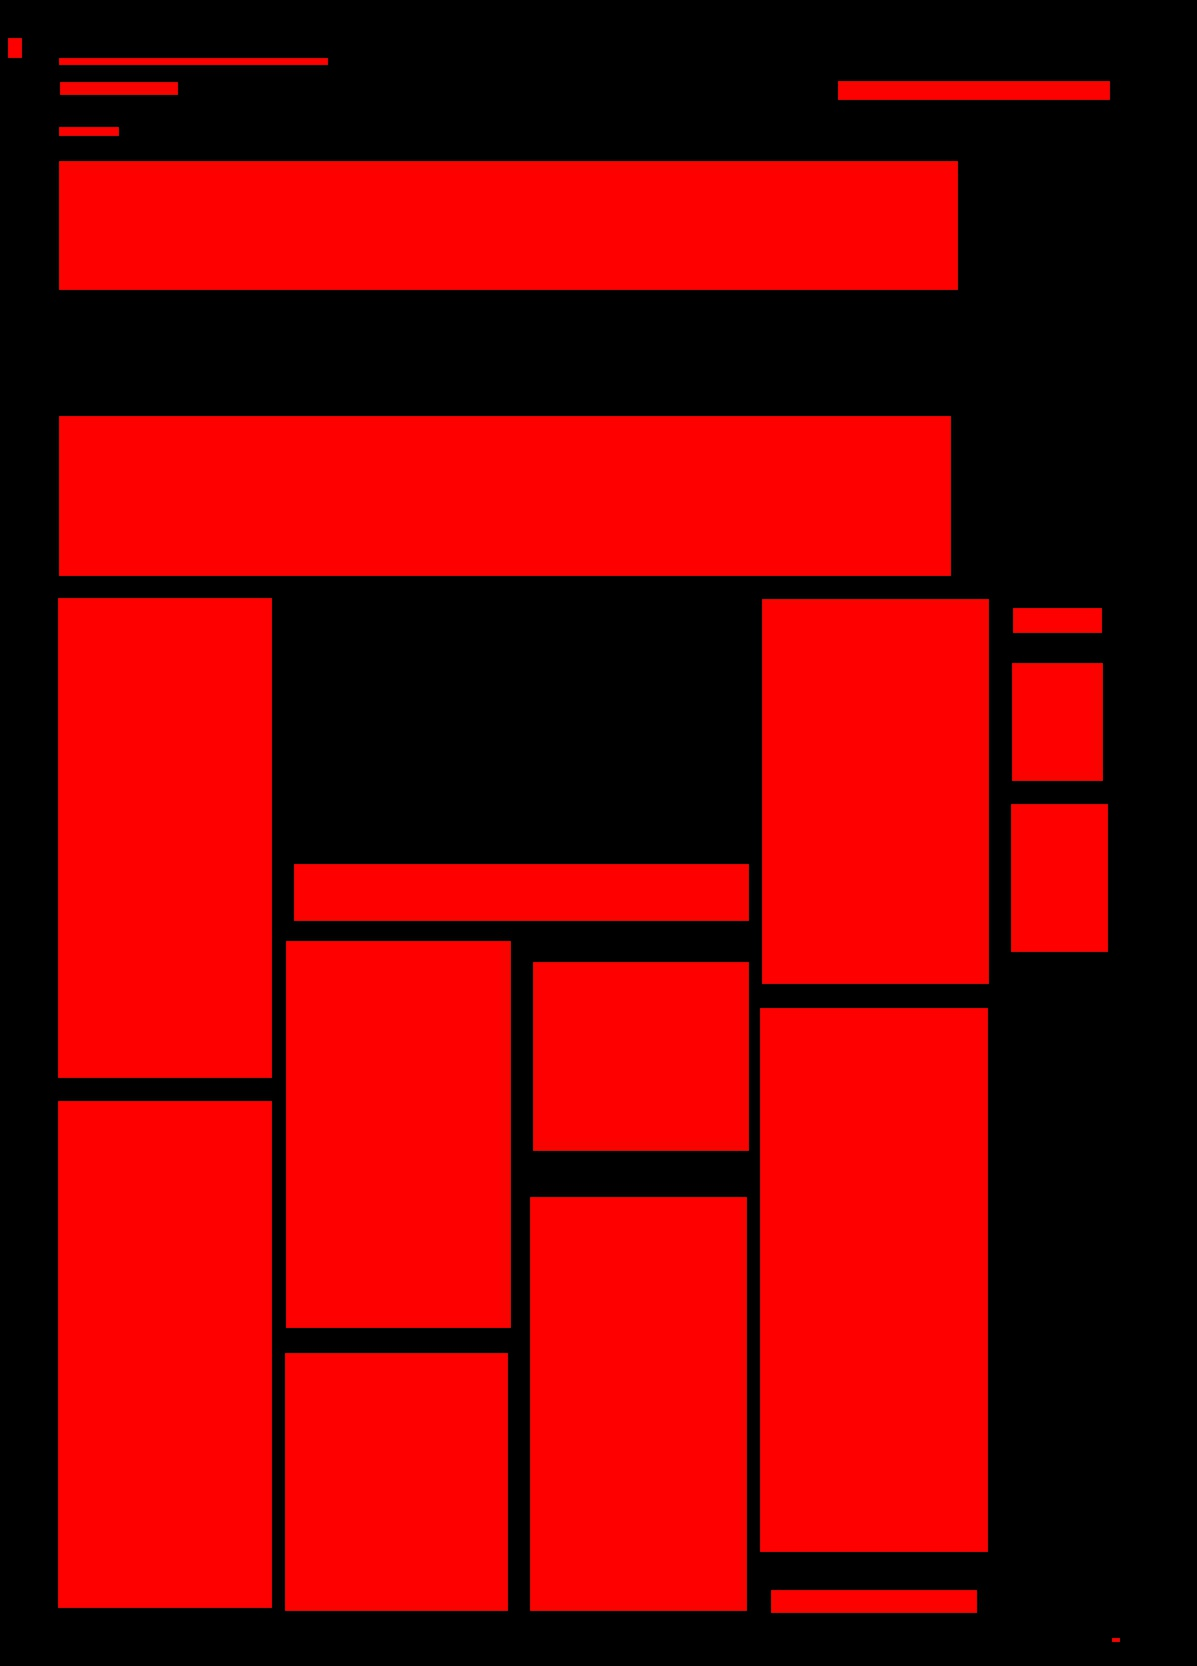
\includegraphics[width=0.99\linewidth, clip=true, trim = 0mm 0mm 0mm 0mm]{figures/ocr/FZKQ4Zg.jpg}
  \caption{OCR}
\end{subfigure}%
\begin{subfigure}{.25\textwidth}
  \centering
  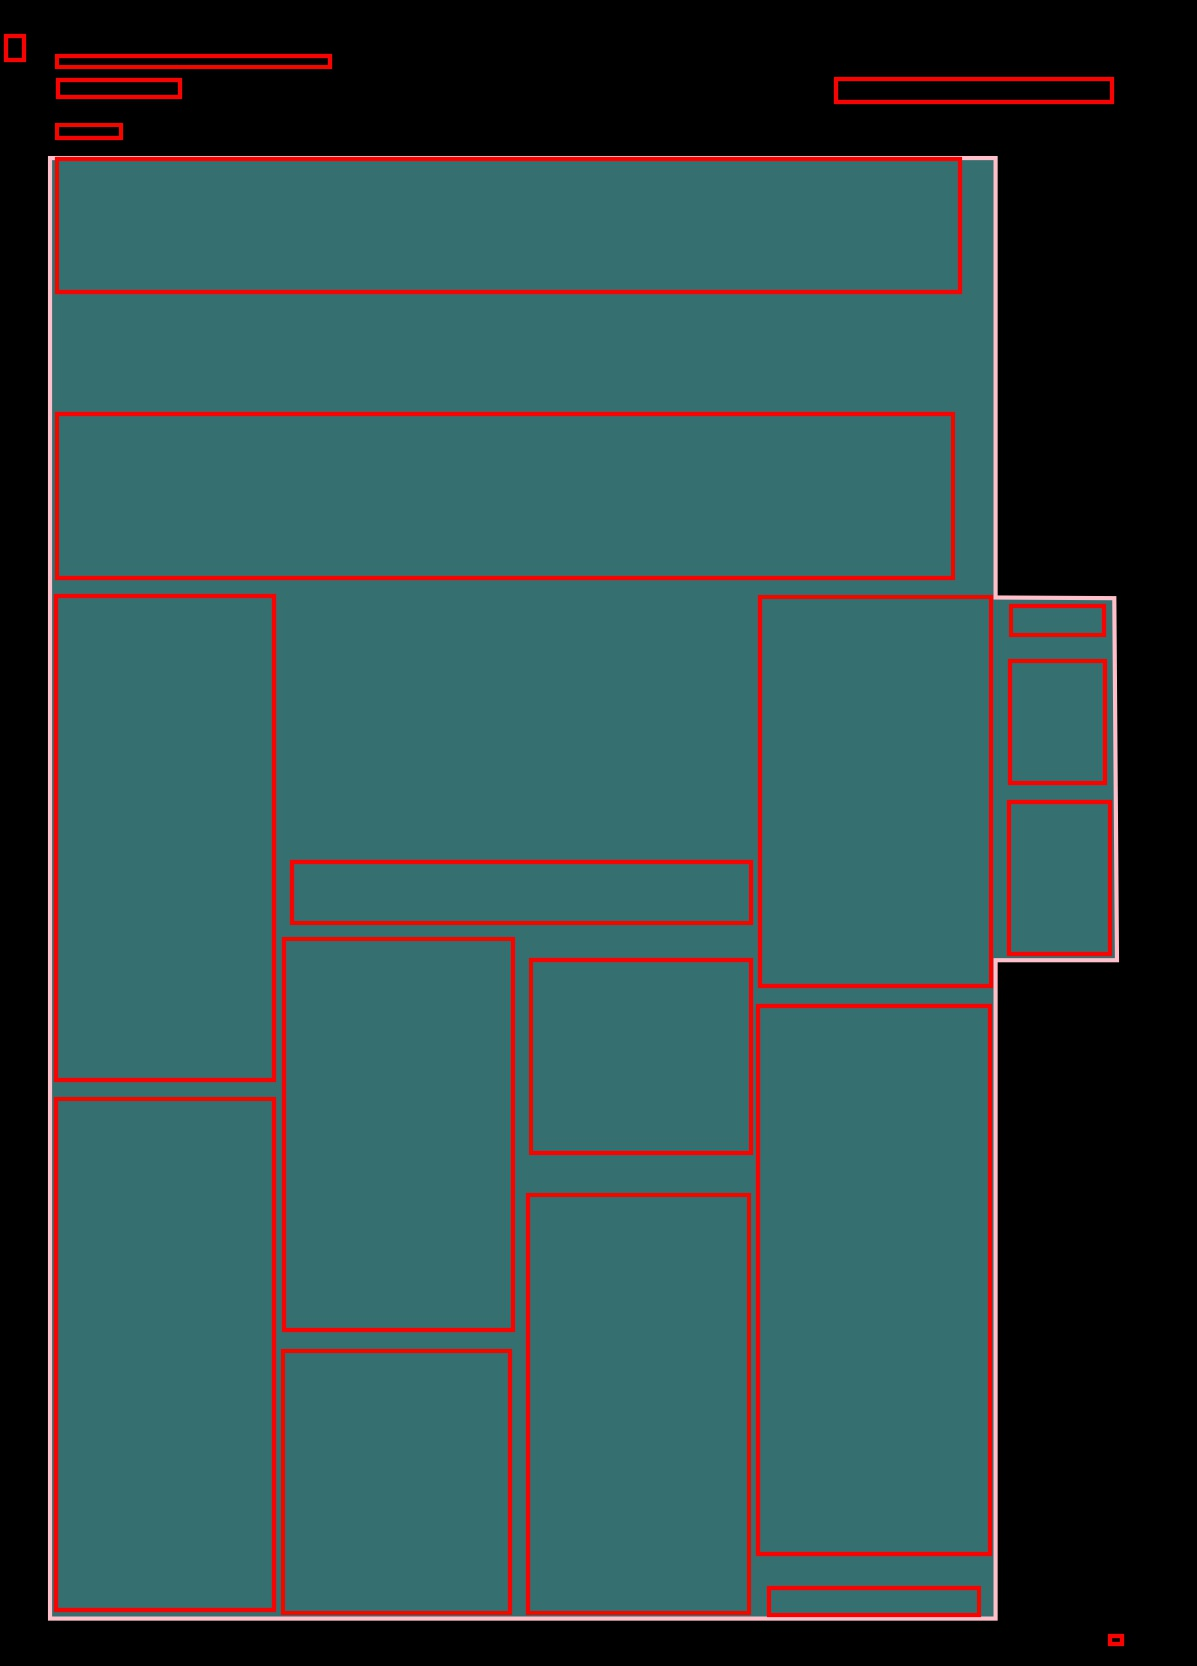
\includegraphics[width=0.99\linewidth, clip=true, trim = 0mm 0mm 0mm 0mm]{figures/ocr_bbox/FZKQ4Zg.jpg}
  \caption{GT Label + OCR}
\end{subfigure}%
\begin{subfigure}{.25\textwidth}
  \centering
  
\includegraphics[width=0.99\linewidth, clip=true, trim = 0mm 0mm 0mm 0mm]{figures/bbox/FZKQ4Zg.jpg}
  \caption{GT Label}
\end{subfigure}%
\begin{subfigure}{.25\textwidth}
  \centering
  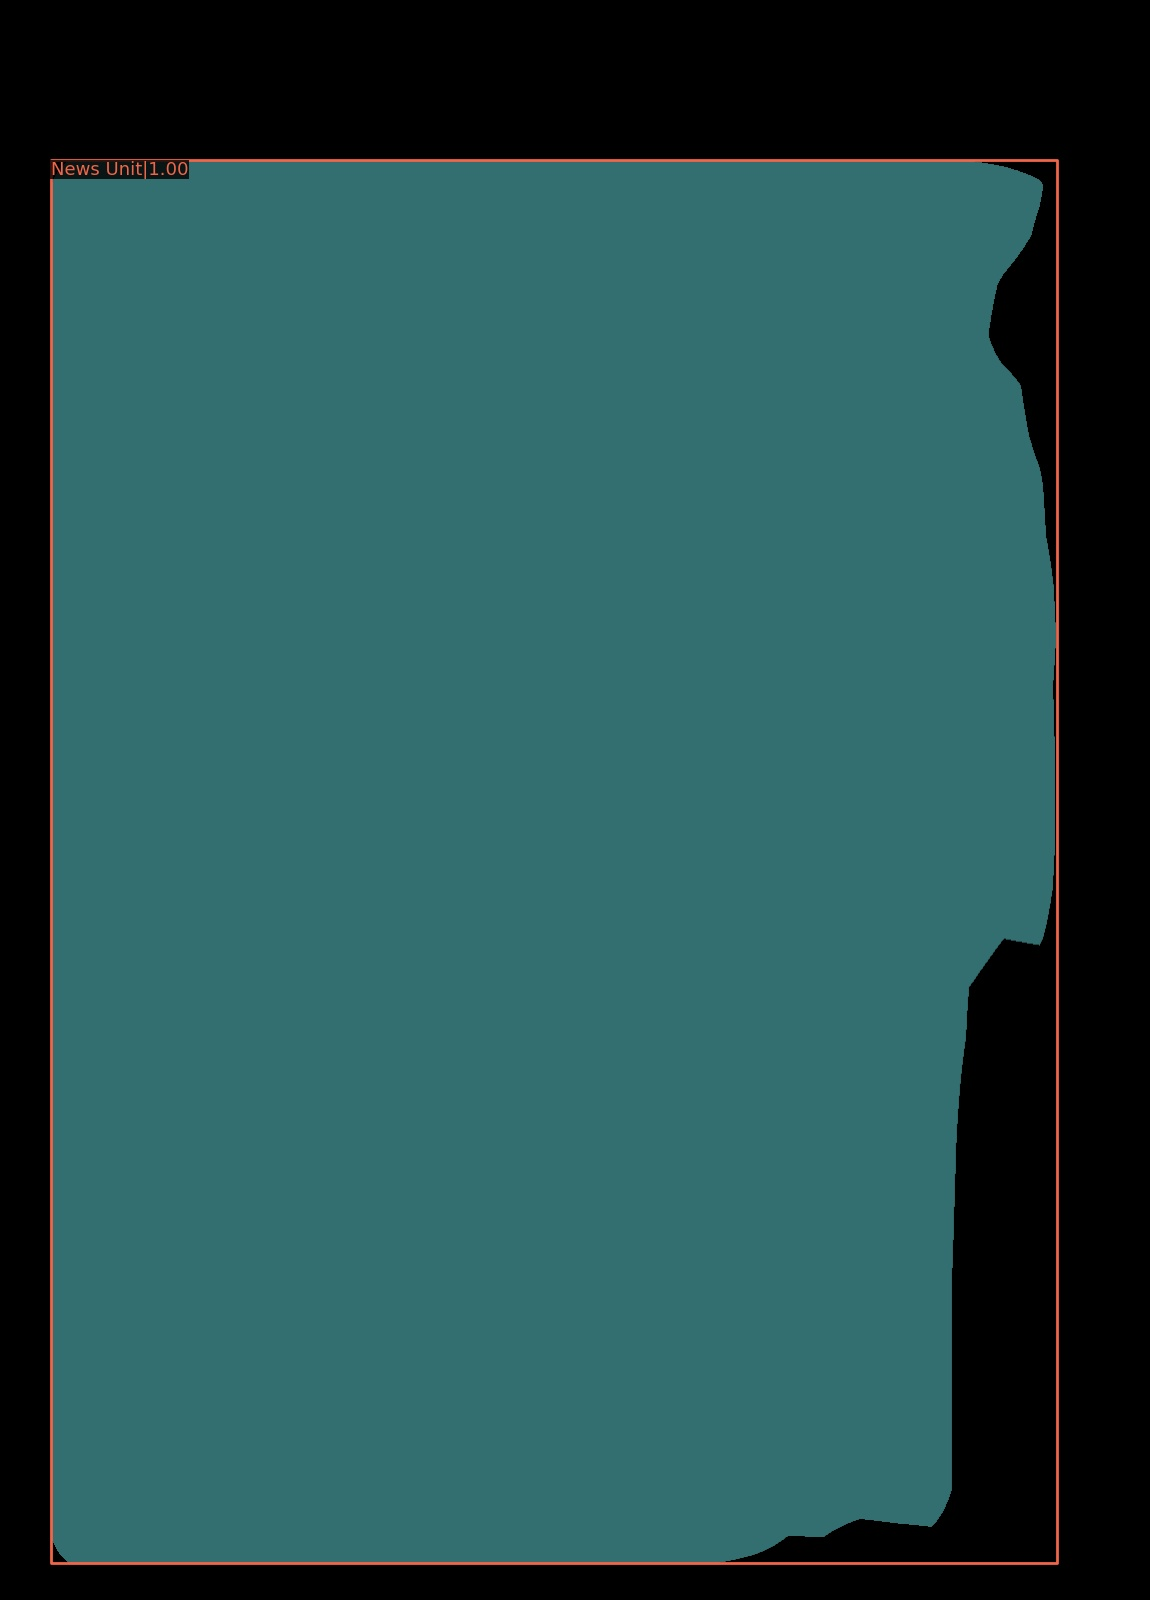
\includegraphics[width=0.99\linewidth, clip=true, trim = 0mm 0mm 0mm 0mm]{figures/labels-vanilla-0.75/FZKQ4Zg.jpg}
  \caption{Model prediction}
\end{subfigure}
\caption{A newspaper page consisting of a large news article: label extension demonstration.}
\label{fig:extendedlabel}
\end{figure}
\end{frame}
\normalpage

%%%%%%%%%%%%%%%%%%%%%%%%%%%%%%%%%%%%%%%%%%%%%%%%%%%%%%%%%%%%
\begin{frame}
  \begin{figure}
\centering
\begin{subfigure}{.25\textwidth}
  \centering
  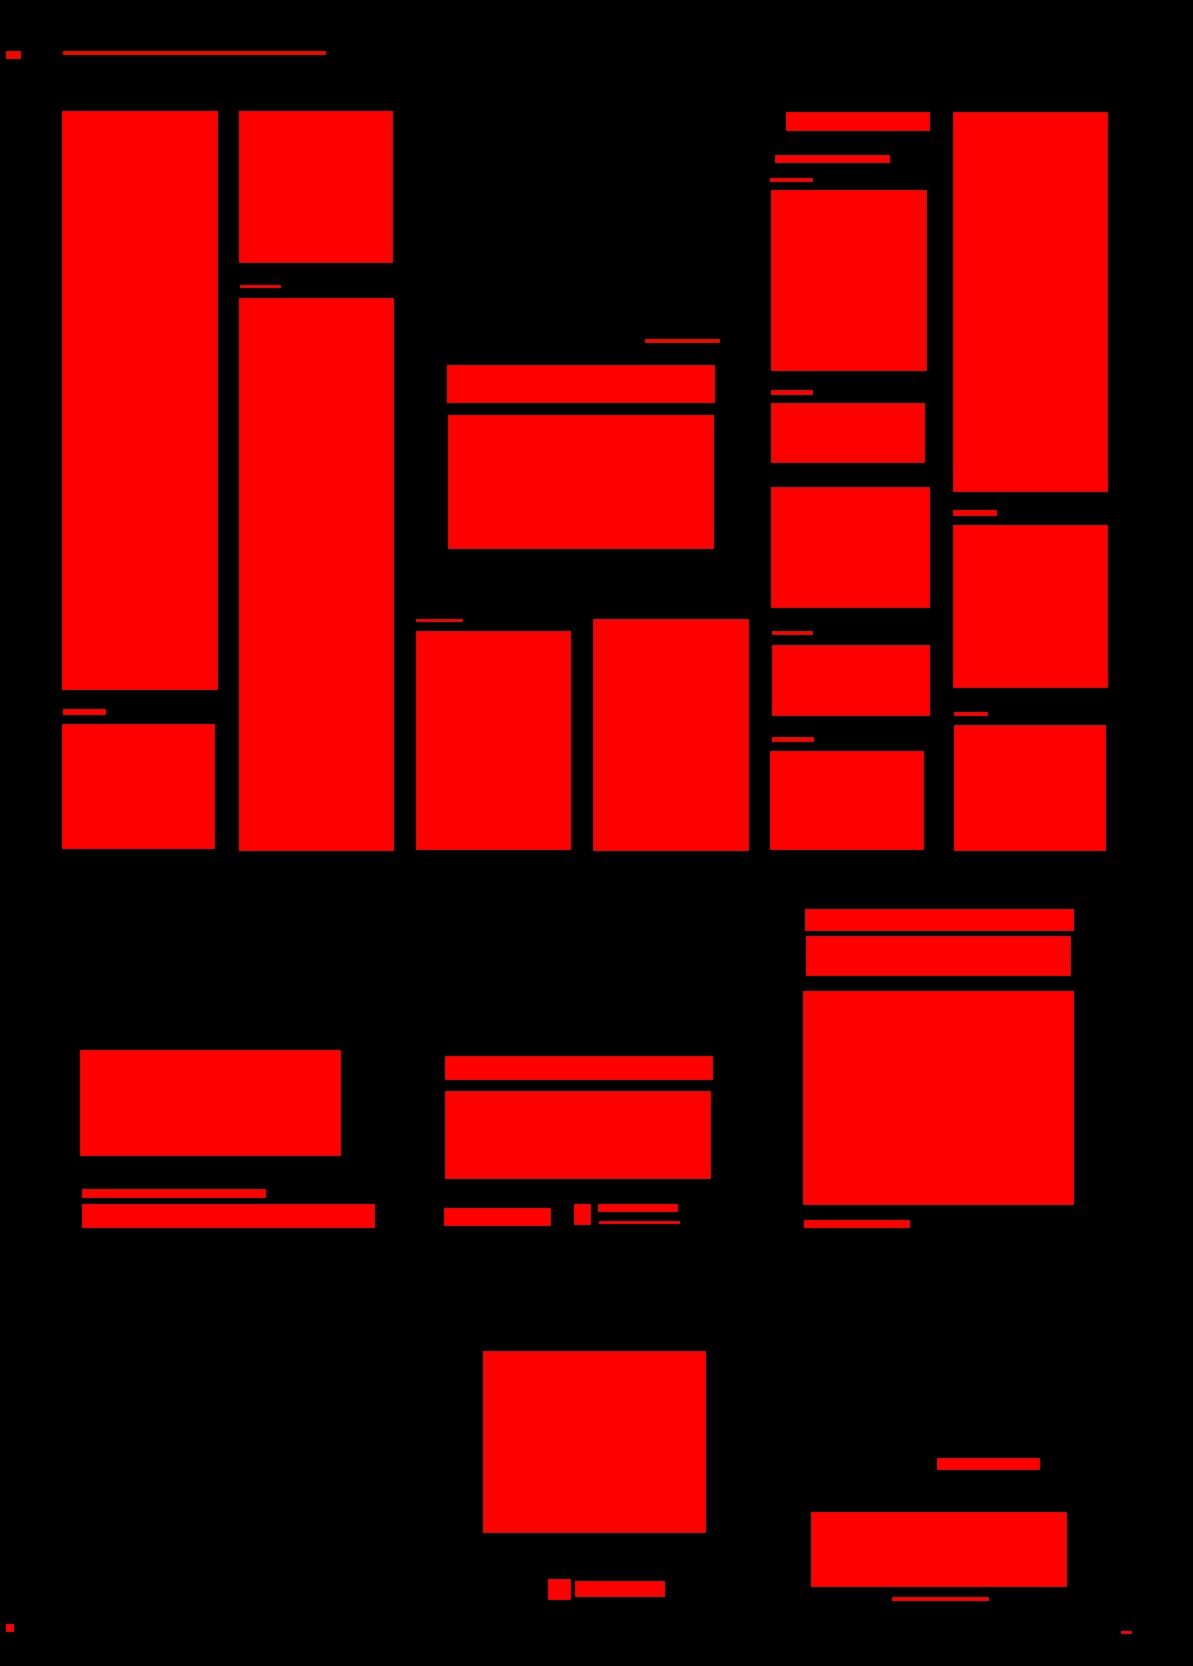
\includegraphics[width=0.99\linewidth, clip=true, trim = 0mm 0mm 0mm 0mm]{figures/ocr/kvtooQ3.jpg}
  \caption{OCR}
\end{subfigure}%
\begin{subfigure}{.25\textwidth}
  \centering
  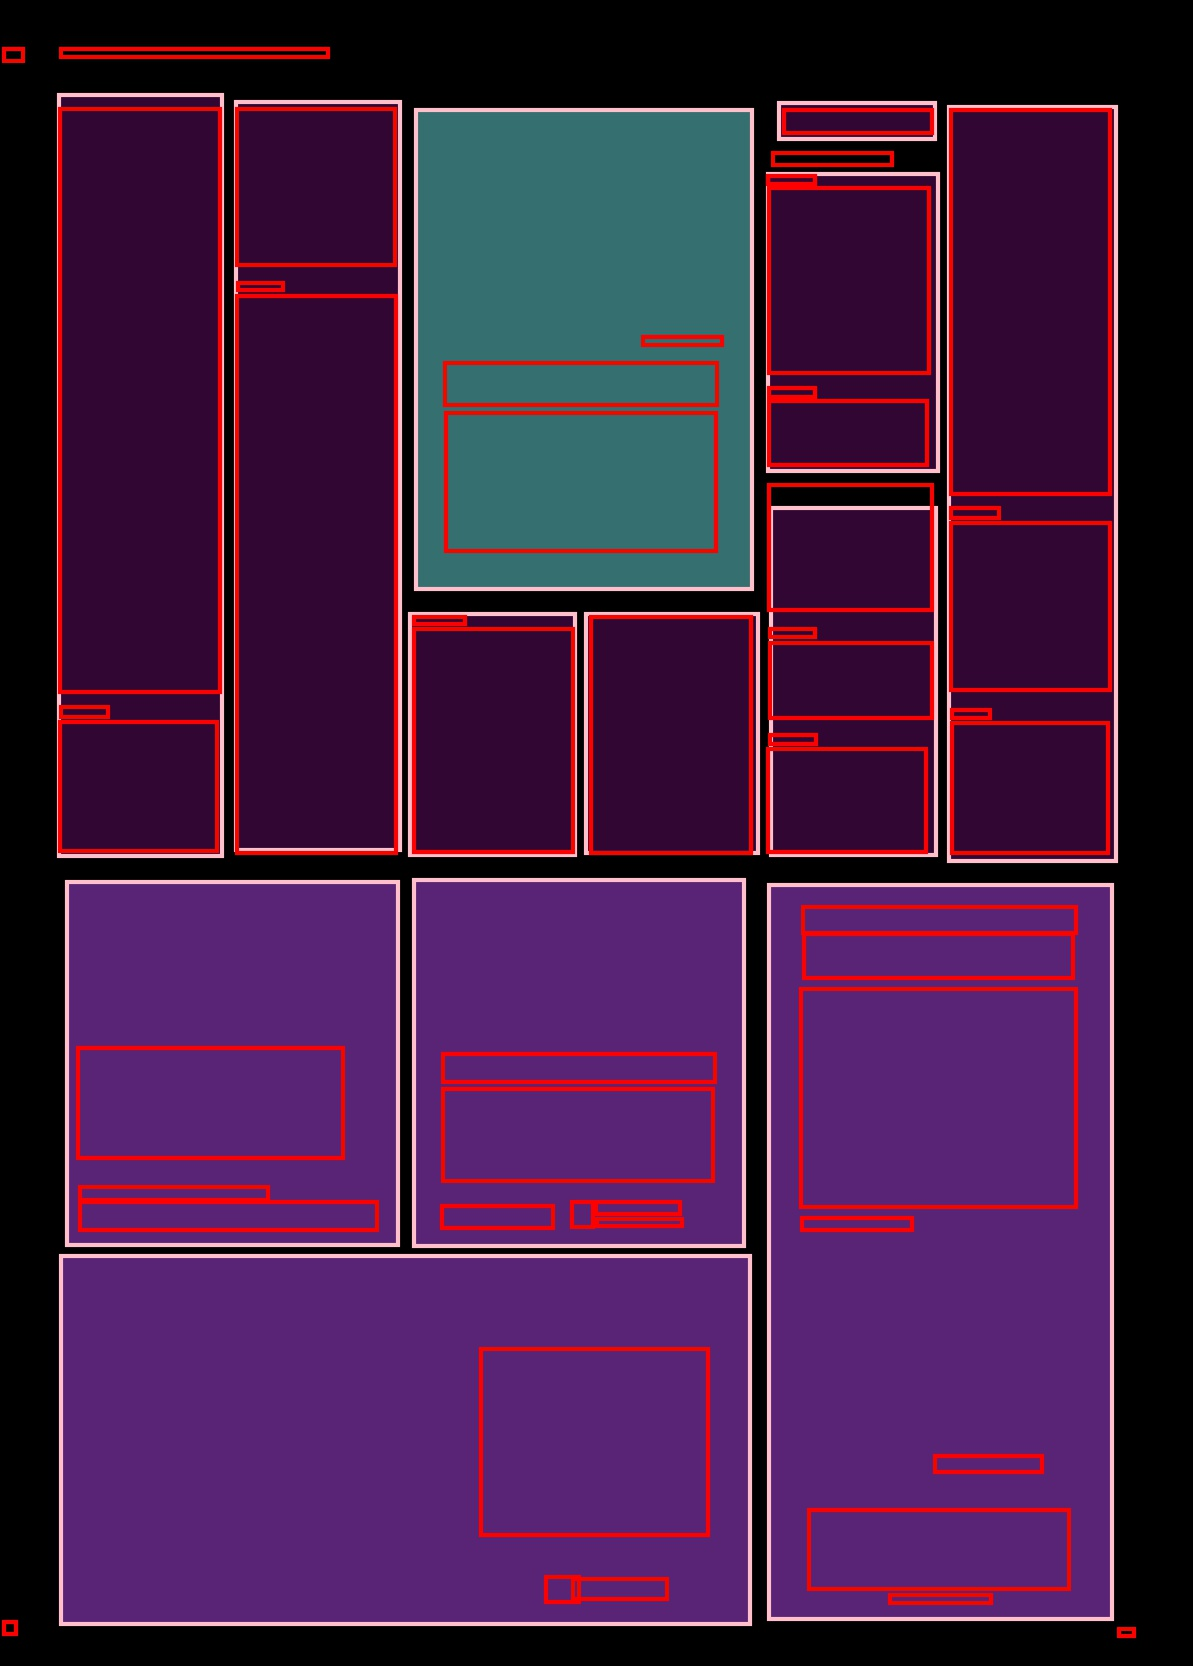
\includegraphics[width=0.99\linewidth, clip=true, trim = 0mm 0mm 0mm 0mm]{figures/ocr_bbox/kvtooQ3.jpg}
  \caption{GT Label + OCR}
\end{subfigure}%
\begin{subfigure}{.25\textwidth}
  \centering
  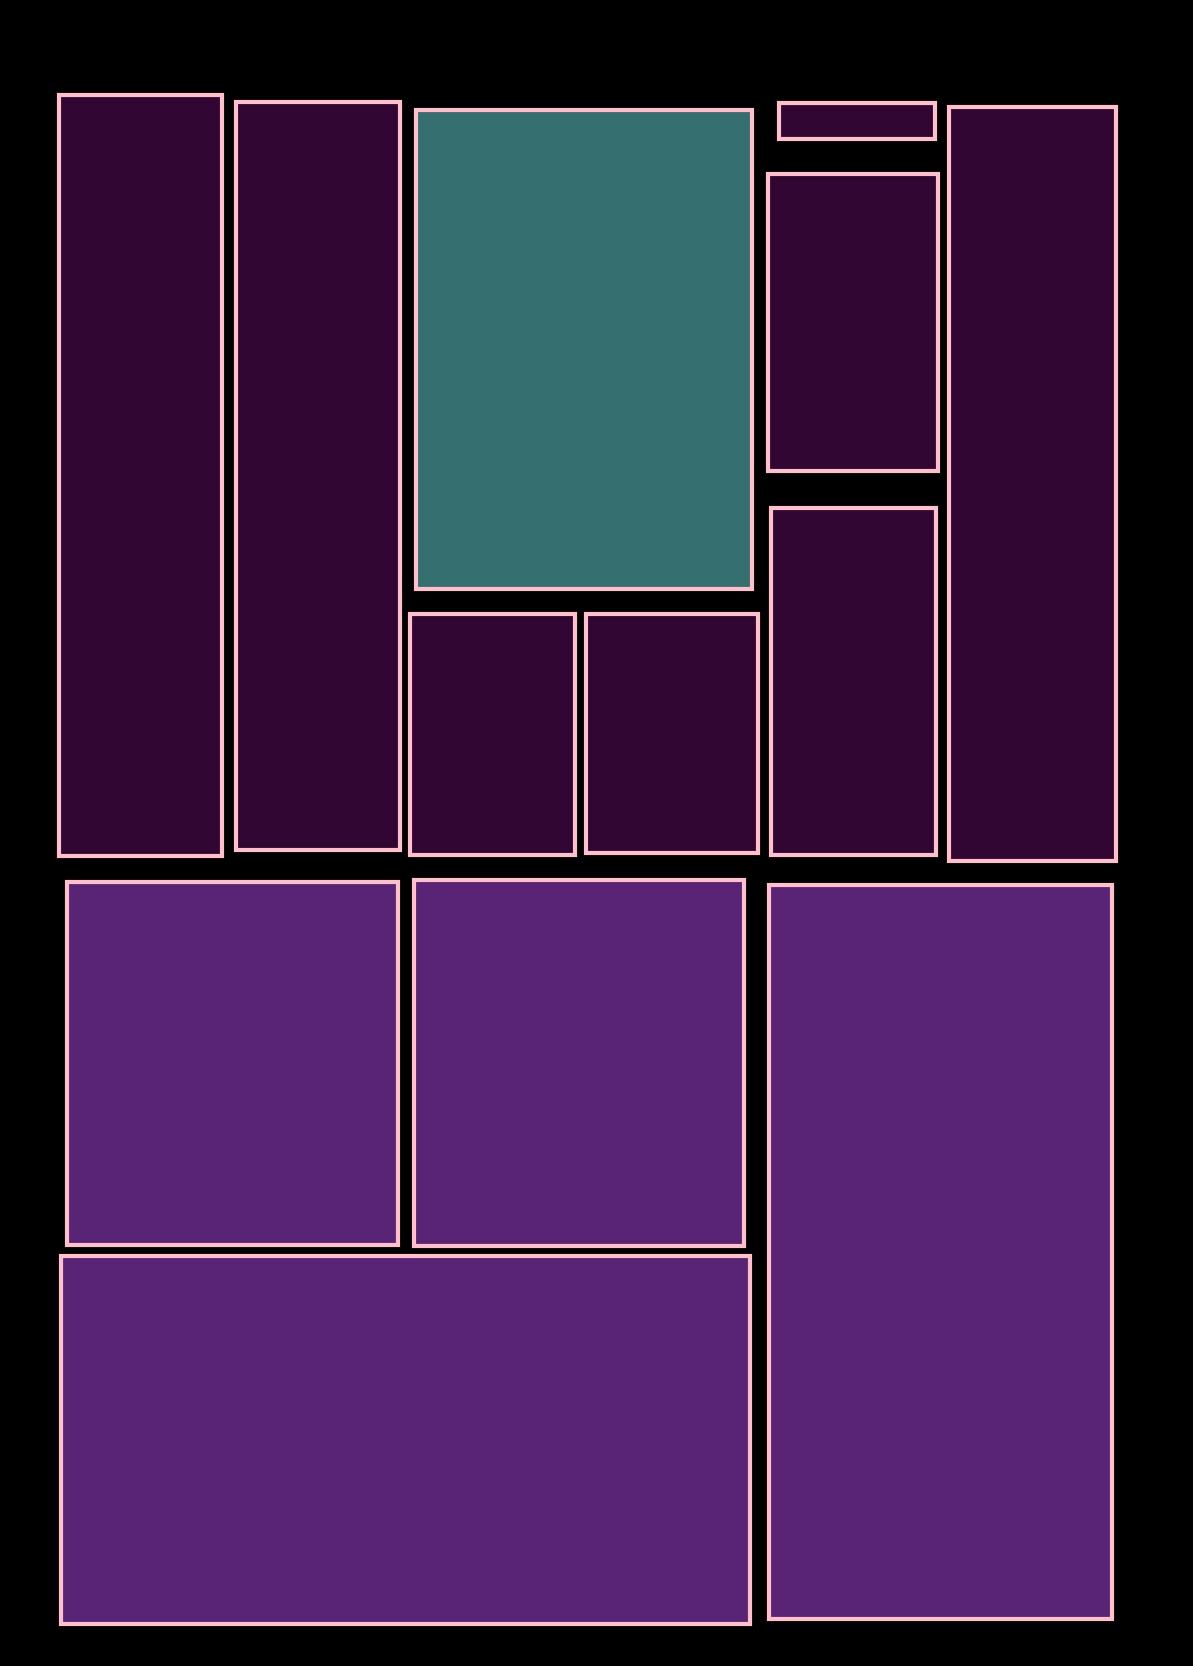
\includegraphics[width=0.99\linewidth, clip=true, trim = 0mm 0mm 0mm 0mm]{figures/bbox/kvtooQ3.jpg}
  \caption{GT Label}
\end{subfigure}%
\begin{subfigure}{.25\textwidth}
  \centering
  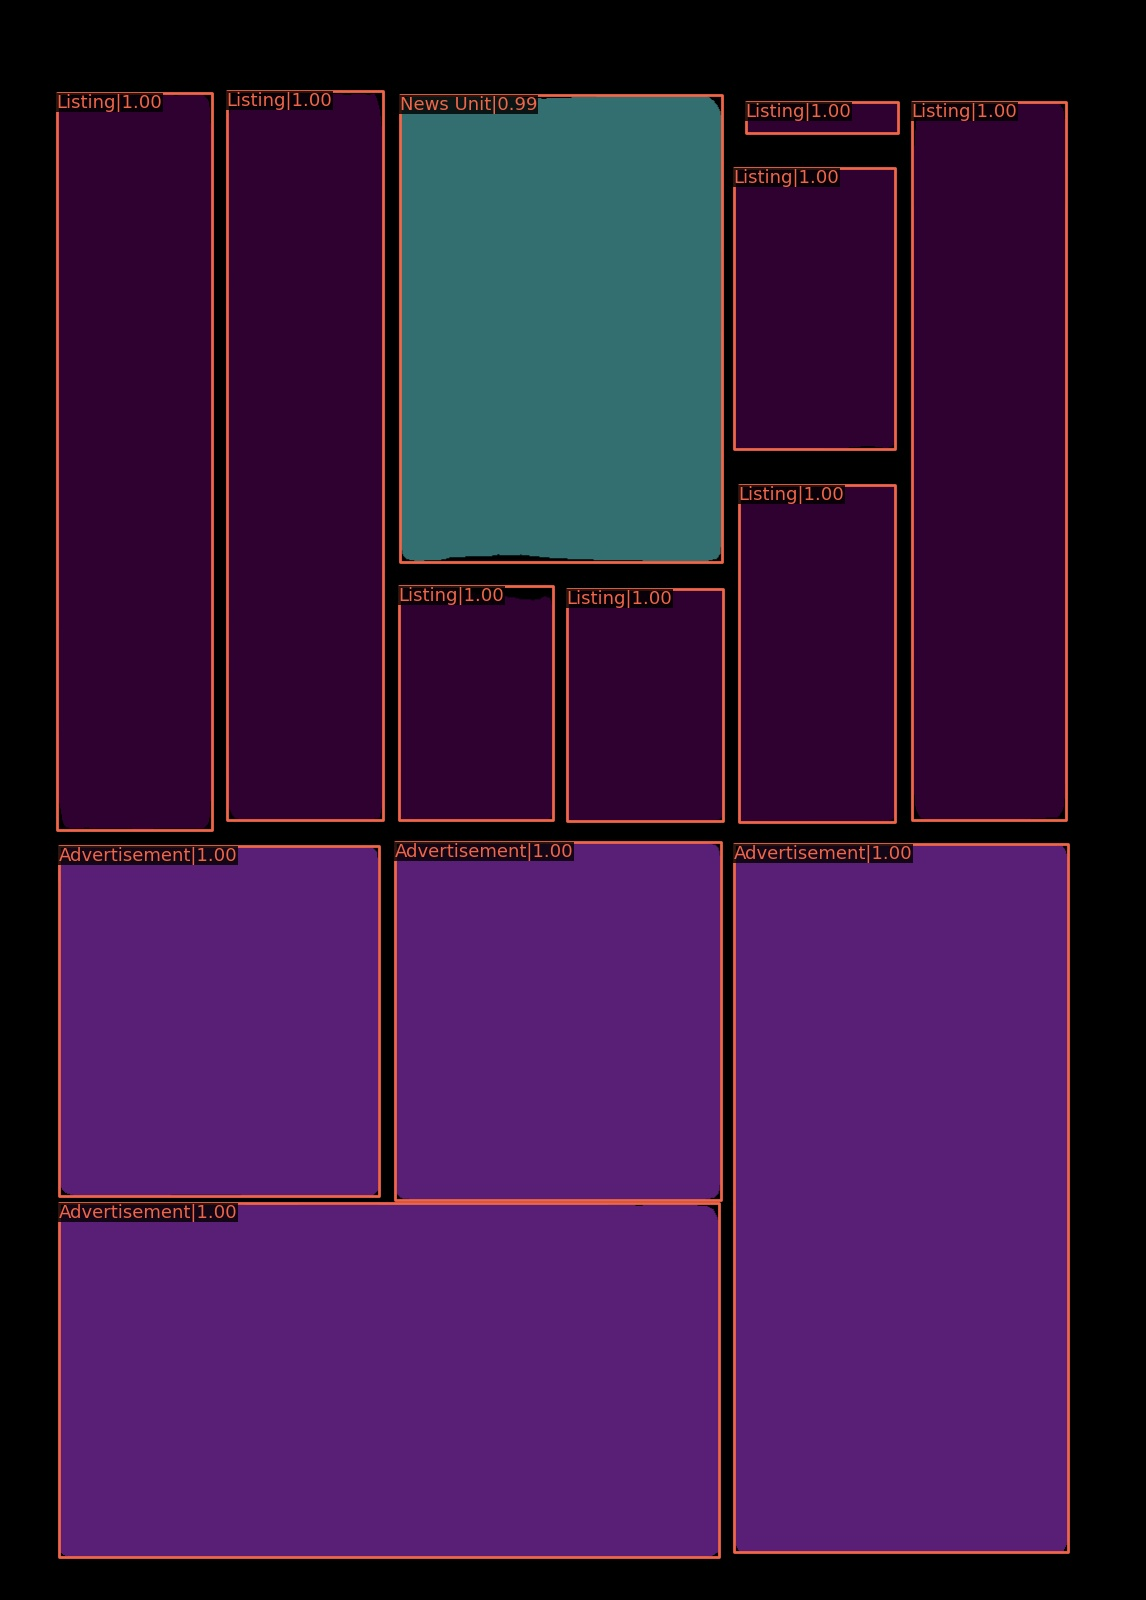
\includegraphics[width=0.99\linewidth, clip=true, trim = 0mm 0mm 0mm 0mm]{figures/labels-vanilla-0.75/kvtooQ3.jpg}
  \caption{Model prediction}
\end{subfigure}
\caption{A newspaper page with event listings.}
\label{fig:extendedlabel}
\end{figure}
\end{frame}
\normalpage


%%%%%%%%%%%%%%%%%%%%%%%%%%%%%%%%%%%%%%%%%%%%%%%%%%%%%%%%%%%%
\begin{frame}
  \begin{figure}
\centering
\begin{subfigure}{.25\textwidth}
  \centering
  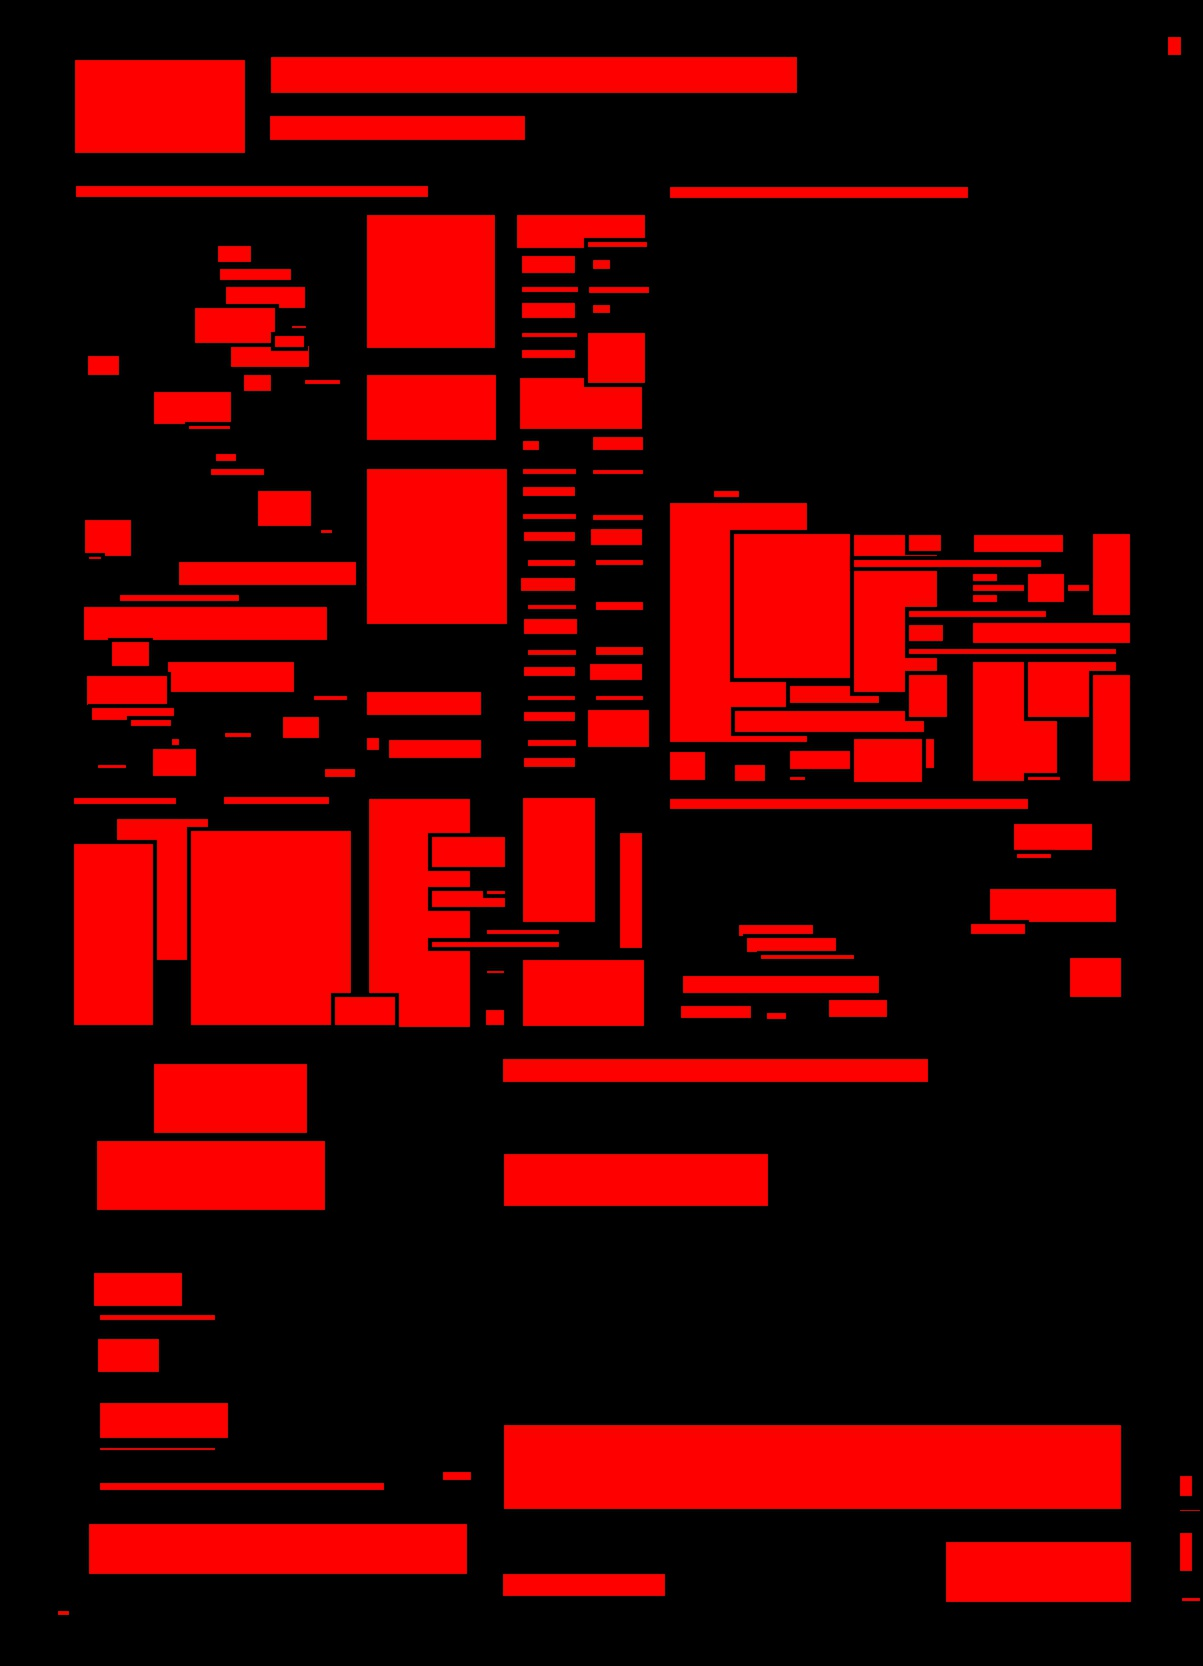
\includegraphics[width=0.99\linewidth, clip=true, trim = 0mm 0mm 0mm 0mm]{figures/ocr/Jd55Bvg.jpg}
  \caption{OCR}
\end{subfigure}%
\begin{subfigure}{.25\textwidth}
  \centering
  \includegraphics[width=0.99\linewidth, clip=true, trim = 0mm 0mm 0mm 0mm]{figures/ocr_bbox/Jd55Bvg.jpg}
  \caption{GT Label + OCR}
\end{subfigure}%
\begin{subfigure}{.25\textwidth}
  \centering
  \includegraphics[width=0.99\linewidth, clip=true, trim = 0mm 0mm 0mm 0mm]{figures/bbox/Jd55Bvg.jpg}
  \caption{GT Label}
\end{subfigure}%
\begin{subfigure}{.25\textwidth}
  \centering
  \includegraphics[width=0.99\linewidth, clip=true, trim = 0mm 0mm 0mm 0mm]{figures/labels-vanilla-0.75/Jd55Bvg.jpg}
  \caption{Model prediction}
\end{subfigure}
\caption{A newspaper page consisting of weather reports and advertisement.}
\label{fig:weather}
\end{figure}
\end{frame}
\normalpage

\end{document}
